\documentclass[11pt,a4paper,titlepage,oneside]{book}

\usepackage[czech]{babel}
\usepackage[utf8]{inputenc}
\usepackage{graphicx}
\usepackage{url}
\usepackage{fancyhdr}
\usepackage{setspace}
\usepackage{hyperref}
\usepackage{rotating}
\usepackage[withpage]{acronym}



%\usepackage{titlesec}
%\titleformat{\chapter}{\normalfont\LARGE\bfseries}{\thechapter}{1em}{}
%\titlespacing*{\chapter}{0pt}{3.5ex plus 1ex minus .2ex}{2.3ex plus .2ex}


\begin{document}
%pro vytváření HTML tagů
\newcommand{\htmlTag}[1]{ \textless #1\textgreater \textless \textbackslash #1\textgreater}
\renewcommand\bibname{Reference}
%nastavení fancy stylu
\lhead{
\includegraphics[height=0.5cm]{obrazky/lev.jpg} {ČVUT v~Praze}}
\rhead{\leftmark}
\cfoot{\thepage}
\setlength{\headheight}{24pt}

\pagestyle{empty}	%%vypne číslování

\begin{titlepage} %% titulní strana 1(bez lva)
	\begin{center}
		{\huge ČESKÉ VYSOKÉ UČENÍ TECHNICKÉ} \\ [0.25cm]
		{\LARGE FAKULTA STAVEBNÍ}
		\\[9cm]		
		{\Huge DIPLOMOVÁ PRÁCE}
		\\[9cm]
		{\Large Praha 2013 \hspace{\stretch{1}} Bc. Chrudoš VORLÍČEK}
	\end{center}
\end{titlepage}

\begin{titlepage} %%titulní strana 2 (se lvem)
	\begin{center}
		{\huge ČESKÉ VYSOKÉ UČENÍ TECHNICKÉ} \\
		{\LARGE FAKULTA STAVEBNÍ \\ [0.25cm]OBOR GEOINFORMATIKA}
		\\[1cm]
		\begin{figure}[!h]
		\begin{center}
		
\includegraphics[height=5cm]{obrazky/lev.jpg}
		\\[1cm]
		\end{center}
		\end{figure}							
		{\Huge DIPLOMOVÁ PRÁCE \\ [0.25cm]}
		{\LARGE \uppercase {Prototyp turistického systému zaloŽeného na datech \\[0.25cm] OpenStreetMap}}
		\\[3.5cm]
		{\Large Vedoucí práce: Ing. Martin LANDA, Ph.D. \\[0.25cm] Katedra geomatiky}
		\\[1cm]
		{\Large Praha 2013 \hspace{\stretch{1}} Bc. Chrudoš VORLÍČEK}
	\end{center}
\end{titlepage}

\newpage %%zadání
	\begin{center}
		\vspace*{15cm}
		{\Large ZDE VLOŽIT LIST ZADÁNÍ}
	\end{center}

%% Abstrakt
\begin{flushleft}
	\chapter*{}
	\section*{ABSTRAKT}
	\paragraph{} Hlavním tématem této práce je tvorba webové turistické aplikace za použití dat OpenStreetMap, jeho napojení na sociální síť Facebook a~přidávání dat přímo do OpenStreetMap. Součástí práce je i stručné shrnutí existujících řešení, popsání užitých technologií a jejich výhod a~nevýhod.
	\section*{KLÍČOVÁ SLOVA}
	{\sc{OpenStreetMap, OSM, Turistický systém, Facebook, Nette, PHP, Geoserver, iD, OpenLayers}}
	\section*{ABSTRACT}
	\paragraph{} The topic of this diploma thesis is to create a prototype of tourism system based on OpenStreetMap and to connect it with social network Facebook. It allows to add or edit objects in OpenStreetMap. The work also includes a brief summary of the existing solutions and describe the technologies and their advantages and disadvantages.
	\section*{KEYWORDS}
	{\sc{OpenStreetMap, OSM, tourism system, Facebook, Nette, PHP, Geoserver, iD, OpenLayers}}
\end{flushleft}

\newpage %%Prohlášení
	\vspace*{15cm}
	\section*{\Large PROHLÁŠENÍ}
		\paragraph{}Prohlašuji, že jsem diplomovou práci na téma \uv{Prototyp turistického systému založeného na datech OpenStreetMap} vypracoval samostatně a~že veškerou použitou literaturu a podkladové materiály uvádím v~seznamu zdrojů.\\[1cm]
	V~Praze dne ....................... \hspace{\stretch{1}}................................. \\
	\hspace*{\stretch{1}} {(podpis autora)\hspace{0.25cm} }
	
\newpage %%Poděkování
	\vspace*{15cm}
	\section*{\Large PODĚKOVÁNÍ}
	\paragraph{} Rád bych poděkoval Ing. Martinu Landovi, Ph.D. za ochotu při vedení diplomové práce, za jeho připomínky a podněty. Dále bych chtěl poděkovat rodině za podporu při celém studiu na VŠ. V~neposlední řadě bych chtěl poděkovat Michalu Odcházelovi za rady při řešení problémů vzniklých při programování aplikace.
		
\renewcommand{\baselinestretch}{1.5} %nastaví mezery
\newpage %%Obsah
\pagestyle{plain}
\pagenumbering{arabic}
\setcounter{page}{5}

	\tableofcontents

\newpage %%Obrázky a tabulky
	\listoffigures

\newpage %%Samotný text
%%Úvod
\chapter*{Úvod}
\addcontentsline{toc}{chapter}{Úvod}

%%% ML: Prvni veta zni velmi kostrbate, zvlaste "a s jeho rozšířením i
%%% do mobilních telefonů je dostupný na mnoha místech". Zkuste cely
%%% odstavec prepsat...

%%% -> ML: OK

	\paragraph{} Mapy byly vždy součástí výbavy cestovatelů. Pomáhaly jim při orientaci v~krajině a volbě vhodné cesty. S~rozvojem počítačů začaly být papírové mapy nahrazovány mapami digitálními. Ty mohou být uloženy na pevném disku serveru a dostupné pomocí internetu nebo jsou uloženy na paměťovém médiu přístroje, který je zobrazuje. Nástup chytrých mobilních telefonů a tabletů spolu s~kvalitním a rychlým připojením k~internetu umožňuje prohlížet webové mapové aplikace prakticky odkudkoliv. Díky tomu můžeme na cestách vyhledávat zajímavé objekty v~našem okolí a informace o~nich. To z~mapových aplikací dělá dobré společníky při plánování výletů či dalekých cest.
	\paragraph{} Stejně tak jako se liší služební cesta od výletu, liší se i potřeby uživatelů. Podnikatel cestující autem, který hledá nejkratší cestu z~bodu A~do bodu B, nepotřebuje pro vyhledávání turistické mapy. Ačkoliv je může použít, obsahují pro něj nadbytečná data a mohou být příliš podrobné. Kdyby turista hledal v~automapě cestu z~bodu A~do B, pravděpodobně by ji našel, ale vedla by nejspíš po silnicích, což není úplně žádoucí. Každá mapa, ať už papírová či internetová, poskytuje různá data. Výhodou internetových mapových aplikací je mimo jiné i možnost zobrazení různých dat v~potřebném měřítku v~jednom mapovém okně.

        %%% ML: Pri prvnim pouziti by mela byt zkratka rozpsana,
        %%% napr. Application Programming Interface (API). Seznam
        %%% zkratek lze generovat automaticky - viz
        %%% http://staff.science.uva.nl/~polko/HOWTO/LATEX/acronym.html

        %%% -> ML: OK

        %%% ML: Na konci odstace "Navíc se většinou jedná o
        %%% doprovodnou funkci." (ceho?) "Výhodou ovšem je snadnější
        %%% tvorba." (tvorba ceho?) Ctenar tape...

        %%% ML: Misto "prostorova data" (prilis obecny pojem)
        %%% pouzivejte radeji "geograficka
        %%% data" ci "geodata", v textu jsem to na nekolika mistech
        %%% jiz opravil

        %%% ML: Tato veta je zmatecna: "Pokud je zobrazování
        %%% geografických dat hlavní náplní aplikace, je lepší použít
        %%% specializovanou aplikaci" - v dalsim textu hovorite "o
        %%% dvou pristupech" - z textu neni zcela jasne cim se lisi
        %%% (viz poznamka vyse) Az z dalsiho textu je zrejme co mate
        %%% na mysli.

        %%% -> ML: text je jiz citelnejsi, prehlednejsi -> OK

	\paragraph{} Portály poskytující mapové aplikace často vytvářejí svá \ac{API}, aby jejich produkty mohly být použity i na jiných serverech. Díky tomu je možné narazit na mapy od Googlu či Seznamu i na jiných stránkách. Jedná se o~nejsnazší způsob, jak prezentovat geografická data, např. společnost zabývající se venkovní reklamou tak může prezentovat rozmístění nabízených billboardů. Tento přístup má ale svá omezení daný funkcemi, které \ac{API} poskytuje. Často je bezplatné užití \ac{API} omezeno i počtem přístupů či velikostí poskytovaných dat. Takto vytvořené mapy mají většinou vizuálně prezentovat slovní popis umístění (např. adresu). Z~českých aplikací je tato metoda použita např. na webu Výletník.cz, viz kap. \ref{sec:vyletnik}.
	\paragraph{}Další možností, jak prezentovat geografická data, je vytvoření specializované aplikace. Tento přístup je výhodný, pokud je zobrazení geodat primárním účelem webu a pokud chceme uživatelům nabídnout i funkce, které \ac{API} některého z~poskytovatelů nepodporuje. 

        %%% ML: "vytvoren" vzorek aplikaci, zkuste najit lepsi slovo

        %%% ML: "Většina nalezených aplikací neumožňuje připojení k
        %%% sociálním sítím." To je potreba nejak dolozit, mel jste na
        %%% mysli "vetsina *zkoumanych* ..."

        %%% -> ML: OK

	\paragraph{} Na internetu lze dohledat několik turistických portálů. Aby v~rámci této práce nebylo vytvářeno něco, co už existuje, byly vybrány a prozkoumány některé mapové aplikace. Tento výběr posloužil k~utvoření přehledu funkcionalit, výhod, nevýhod a~originálních prvků webových mapových aplikací. Více je popsáno v~kapitole \uv{Existující řešení}, viz kap. \ref{sec:Ex_reseni}. Většina zkoumaných aplikací neumožňuje připojení k~sociálním sítím. V~současné době, kdy jsou sociální sítě jako Facebook a~Twitter velmi rozšířené, mohou být funkce jako přihlášení přes už existující účet či sdílení výletních tras s~přáteli přidanou hodnotou aplikace. 

        %%% ML: Aplikace je postavena nad daty projektu
        %%% OpenStreetMap. - to nelze definovat jako cil, a uz vubec
        %%% ne na prvnim miste, jde spise "o zakladni vlastnosti
        %%% navrzene webove aplikace, ktera vznika jako prakticky
        %%% vystup teto prace..."

        %%% -> ML: OK

	\paragraph{} Cílem této práce je vytvoření prototypu turistického systému, který bude splňovat následující vlastnosti:
		\begin{itemize}
			\item Uživatelé systému mohou použít svůj účet na sociální síti \ac{Fb}.
			\item Uživatel přihlášený pomocí \ac{Fb} může na \acl{Fb}u zveřejňovat mapy.
			\item Přímo ze stránek mohou přihlášení uživatelé editovat data \ac{OSM}.
			\item Registrovaní uživatelé mohou přidat vlastní trasy. Jakýkoliv přihlášený uživatel může tyto trasy okomentovat.
			\item Registrovaní uživatelé mohou vkládat do mapy fotografie.
		\end{itemize}
	\paragraph{} Protože v~mapách často něco hledáme, měla by vyvíjená mapa umožnit uživatelům vyhledávat objekty a cesty z~bodu A~do bodu B. Vyhledávání by mělo zahrnovat i pokročilé volby, kdy se dá vyhledat zájmový bod v~určité vzdálenosti od plánované cesty či od jiného bodu. Tyto body mají až druhotný význam a budou realizovány pouze v~případě, že hlavní funkcionality projektu budou bez problému fungovat.

        %%% ML: Veta "Bude zmíněna jeho historie, možnosti, kvalita a
        %%% výhody a nevýhody." zni divne, kvalita ceho...? vyhody
        %%% nevyhody - pro co? nebo silne ci slabe stranky

        %%% ML: """Množství programů a programovacích jazyků, které
        %%% lze použít, je velké." pro co? Nemel by to byt novy odstavec?

        %%% ML: piste konkretne: pouzity *pro vyvoj predkladane webobe
        %%% aplikace*, jeji vyvoj a pod

        %%% ML: Též zde lze najít popsaný výsledný stav aplikace ke dni
        %%% dokončení práce. Přeformulujte, nezni to cesky...

        %%% -> ML: OK

	\paragraph{} Práce je strukturována do pěti kapitol. V~první kapitole se text věnuje existujícím řešením. Prozkoumáním aplikací bylo zjištěno, jaké funkce jsou obvykle k~dispozici a jaké nikoliv.
	\paragraph{} Druhá kapitola je věnována  komunitnímu projektu \ac{OSM}. Bude zmíněna jeho historie, možnosti a přesnost a úplnost zobrazených dat. V~této kapitole budou popsána i data \ac{OSM}. 
	\paragraph{}Třetí kapitola je zaměřena na technologickou stránku problému. Množství programů a programovacích jazyků, které pro vytvoření mapové aplikace lze použít, je velké. Proto v~této části budou popsány jen ty programy, jazyky a~knihovny, které byly použity či  jejichž použití bylo zvažováno.
	\paragraph{}Ve čtvrté části práce je popsán vývoj aplikace a s~ním spojené problémy. Je zde také její stav v~době odevzdání práce. 
	\paragraph{}V poslední, páté kapitole je zhodnocení celého projektu, odůvodnění koncového stavu aplikace a nápady na její rozšíření, vylepšení či dodělání.
	
\pagestyle{fancy}

%%%%%%%%%%%%%%%%%%%%%%%
%%%%% EXISTUJÍCÍ ŘEŠENÍ 	   %%%%%
%%%%						      %%%%
%%%							  %%%
%%								     %%
%									 %
\chapter{Existující řešení}
	\label{sec:Ex_reseni}
	\paragraph{} Z~velkého množství různých mapových aplikací bylo vybráno šest příkladů, které mají nějakou spojitost se zpracovávaným tématem. Kromě dvou v~České republice nejčastěji užívaných mapových portálů GoogleMaps a Mapy.cz byly pro hodnocení zvoleny tři aplikace postavené nad daty \ac{OSM}. Jedná se o~české aplikace OpenTrackMap a MTB mapa Evropy. Trojici uzavírá web Waymarked Trails. Poslední aplikací je už v~úvodu zmiňovaný Výletník.cz, jehož mapová aplikace je vytvořena pomocí Google \ac{API}. Každá z~těchto aplikací je něčím specifická, má své výhody i nedostatky. 
	\section{Google Mapy}
		\url{http://www.google.com/maps/preview}

                %%% ML: nektere pojmy by bylo zahodno vysvetlit, napr. Street View
                
                %%% ML: jaka data lze napriklad sdilet

                %%% -> ML: OK

		\paragraph{} V~globálním měřítku asi nejužívanější mapovou aplikací jsou Google Mapy spuštěné v~roce 2005. Ve stejném roce společnost Google uvedla k~mapám i \ac{API} pro jejich použití na webech třetích stran. Podle typu užití se jedná buď o~placenou, či volně dostupnou službu. Google má k~mapám velké množství doplňkových funkcí -- od vyhledávání míst přes vyhledávání cest autem, na kole či pěšky po Street View, které poskytuje panoramatické pohledy z~daného bodu, zobrazení 3D modelů budov a fotografií z~momentálně zobrazené oblasti. Též lze importovat data\footnote{Body, linie a polygony.} ve formátu \ac{KML}\footnote{Formát založený na \ac{XML}, který je primárně určen pro sdílení geodat.} a sdílet je s~jinými uživateli.

                %%% ML: "která je na s mapami provázána" ??? 

                %%% -> ML: OK

		\paragraph{} Google Mapy sice jsou užitečným pomocníkem při plánování cest a zobrazení prostorových dat, ovšem jejich užití je pro turisty dosti omezené. Aplikace nedisponuje údaji o~turistických stezkách. Důvodem, proč se mapy od Googlu dostaly do tohoto výběru, je aplikace Panoramio, která je s~Google Mapami provázána. Jedná se vrstvu lokalizovaných fotografií, které uživatelé nahráli do aplikace. Možnost nahrát fotografie do mapy sice poskytují i  Mapy.cz, ovšem aplikace Panoramio je starší -- vznikla v~roce 2005. Původně nebyla vlastněna Googlem, ten ji získal v~roce 2007 a v~roce 2008 byla propojena s~mapovou aplikací. 

                %%% ML: chybi vystleni zkratek, WGS, EPSG a pod

                %%% -> ML: OK

                %%% -> ML: projekce je v češtině zavádějící, přepsal jsem to jako zobrazení

		\paragraph{}  Google vytvořil pro své mapy i nové zobrazení, které vychází z~Mercatorova zobrazení. Pro zobrazení jsou použity vzorce pro Mercatorovo zobrazení na kouli, ale objekty mají  souřadnice v~systému \ac{WGS 84}, což vede k~tomu, že zobrazení není konformní\cite{google_wiki}\label{google_mercator}. Toto zobrazení má několik kódů, kterými je označováno. Původně \ac{EPSG} odmítla zařadit Googlem vytvořené zobrazení do své databáze, proto bylo označeno jako 900913\footnote{Název Google zapsaný v~jazyce leet, ve kterém se některá písmena nahrazují číslicemi.}. Později bylo toto zobrazení přidána do datasetu souřadnicových systémů \ac{EPSG} pod označením EPSG:3857\cite{sphericalMercator}.

		\begin{figure}[!h]
			\begin{center}
				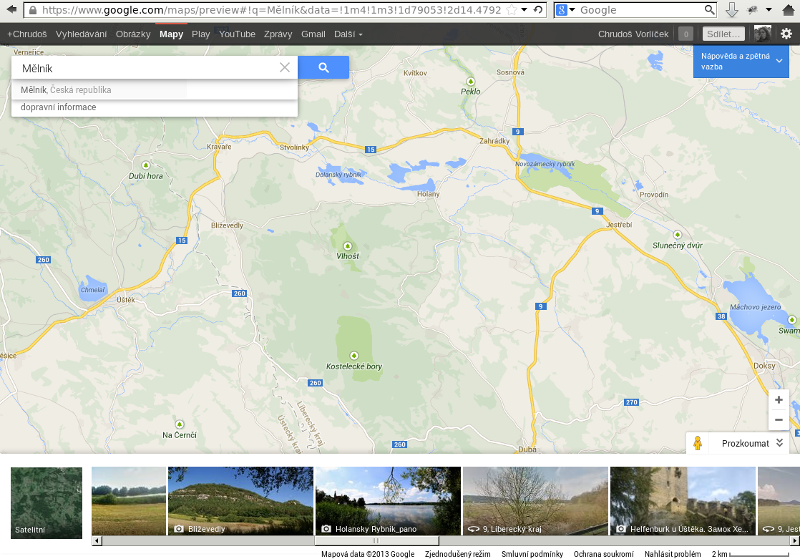
\includegraphics[width=12cm]{obrazky/googleMaps.png}
				\caption{Google Mapy s~přehledem obrázků}
				(zdroj:Google Mapy\cite{googleMap})
			\end{center}
		\end{figure}

\newpage
	\section{Mapy.cz}
		\url{http://mapy.cz/}
			\begin{figure}[!h]
				\begin{center}
					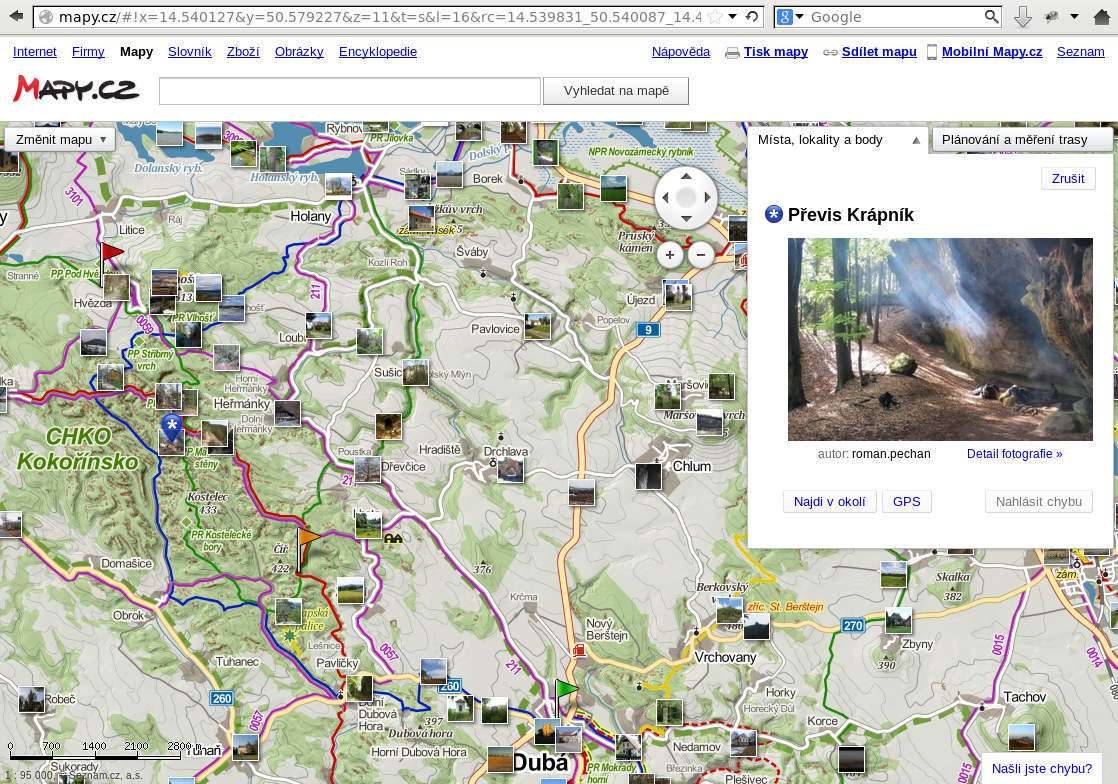
\includegraphics[width=12cm]{obrazky/mapycz.png}
					\caption{Turistická mapa na Mapy.cz}
					(zdroj: Mapy.cz\cite{seznamMapa})
				\end{center}
			\end{figure}

		\paragraph{} I~když je Google se svými mapami světově nejužívanější, v~českých pod\-mínkách mu může konkuruje mapová aplikace firmy Seznam. Mapy.cz mají oproti Googlu výhodu domácího prostředí a zaměření zejména na Českou republiku, což v~důsledku znamená rychlejší aktualizaci mapových podkladů. Mapy.cz poskytují tři různé podkladové mapy (leteckou, obecnou a turistickou) a různé tématické vrstvy (turistické trasy, cyklotrasy, dopravní informace, zastávky MHD a veřejné dopravy aj.). 
		\paragraph{} Na Mapách.cz mohou řidiči, cyklisté a chodci vyhledat trasy z~bodu A~do bodu B přes libovolný počet mezilehlých bodů. V~závislosti na zvoleném dopravním prostředku bere vyhledávač v~potaz i lesní cesty a turistické trasy. Ve stejné záložce lze najít i ruční měření vzdálenosti. Vyhledaná či ručně zadaná cesta může být exportována. Též lze zobrazit její výškový profil. Do mapy lze přidat vlastní body a ty sdílet s~ostatními uživateli pomocí URL adresy. Stejně jako Google poskytuje i Seznam možnost vyhledávat místa podle souřadnic, ulice či názvu objektu. Mapy.cz podporují vkládání fotografií a jejich komentování, ale na rozdíl od Googlu to není řešené jinou aplikací, ale je to přímo součástí aplikace.

	\section{Výletník}
		\label{sec:vyletnik}
		\url{http://mapy.vyletnik.cz/}

		\paragraph{} Turistický portál Výletník.cz poskytuje informace o~možných cílech výletů, o~službách spojených s~turistikou (např. restaurace či ubytování)  či o~zají\-mavých akcích. Díky těmto datům je portál dobrým zdrojem nápadů, pokud připravujeme výlet. Registrovaným uživatelům poskytuje portál informace o~akcích probíhajících následující víkend. Též uživatelům umožňuje vkládat vlastní fotografie, místa a příspěvky. Při registraci je inzerována možnost registrace pomocí Facebooku, ale nikde na to nebyl nalezen odkaz. Nakonec se ukázalo, že Adblock, doplněk prohlížeče Firefox blokující reklamy, vyhodnotil přihlašovací nástroj pro Facebook jako reklamu a podle toho s~ním zacházel. Po vypnutí Adblocku propojení s~Facebookem bylo viditelné. Na druhou stranu se objevilo množství reklam, které kazí jinak dobrý pocit z~webu.

                %%% -> ML: tento obrazek presunut ze sekce Mapy.cz,
                %%% kde byl umisten ponekud nelogicky

		\begin{figure}[!h]
			\begin{center}
				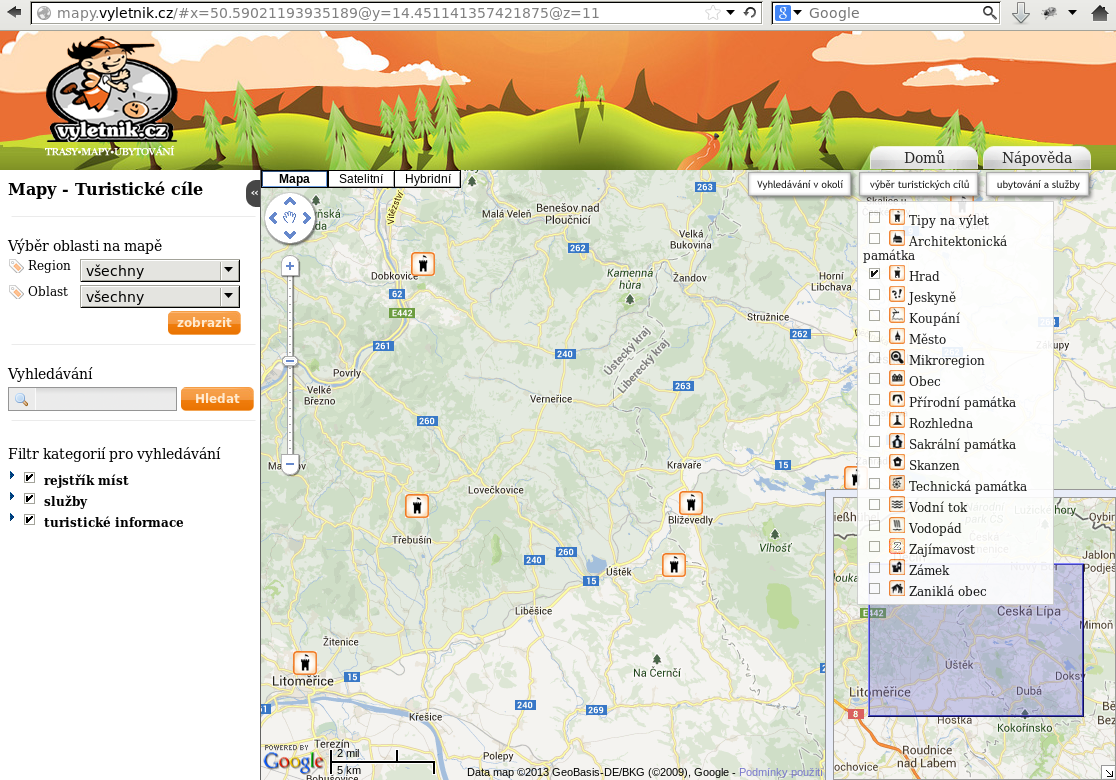
\includegraphics[width=12cm]{obrazky/vyletnik.png}
				\caption{Mapová aplikace portálu Výletník}
				(zdroj: Výletník.cz\cite{vyletnikMapa})
			\end{center}
		\end{figure}


		\paragraph{} Pro mapovou aplikaci tohoto portálu platí to, co pro celý web -- všudy\-přítomné reklamy snižují přívětivost aplikace. Na několika místech se projevilo špatné nastavení stylů aplikace, kdy se prvky překrývaly. Nejzřetelněji je to vidět na možnosti přepínání map. V~nápovědě\cite{vyletnik} je napsáno, že aplikace poskytuje normální, satelitní a hybridní podkladovou mapu, ale možnost přepínání těchto map je překryta rozbalovacími seznamy zájmových bodů. Těch je k~dispozici velké množství a jsou rozděleny na dvě základní skupiny -- \textit{turistické cíle} a \textit{ubytování a služby}. Obě skupiny obsahují další možnosti, ze kterých lze zvolit jednu či více položek. Výletník.cz umožňuje uživatelům vyhledávat objekty ve třech kategoriích:
			\begin{itemize}
				\item rejstřík míst,
				\item služby,
				\item turistické informace.
			\end{itemize}
Vyhledávat lze i v~určitém okruhu od zvoleného bodu.
		\paragraph{} Ačkoliv tato aplikace poskytuje solidní informace, má jistá omezení vyplý\-vající z~toho, že je vytvořena pomocí GoogleMaps \ac{API}. Jednou z~nevýhod jsou chybějící turistické a cykloturistické trasy. Google mapy tyto informace neposkytují a aplikace samotná je z~jiných zdrojů nezískává, čímž vzniká nutnost pro užití dalších portálů pro plánování výletu.	
	
	\section{Waymarked Trails}
		\label{sec:waymarked}
		\url{http://waymarkedtrails.org/cs/}

                %%% ML: "Největší množství dat je v Evropě, zbylé
                %%% části světa jsou z velké části bez dat, ikdyž
                %%% občas nějaká data obsahují. Nejvíce dat je
                %%% poskytují vrstvy s turistickými a
                %%% cykloturistickými stezkami" - zkuste cele
                %%% preformulovat, nezni to prilis cesky

                %%% -> ML: OK
                
		\paragraph{} Aktuální přehled stezek pro turistiku, cykloturistiku a jízdy na inline bruslích je možno najít na mapě Waymarked Trails\cite{Waymarked}. Tato aplikace je vytvořena nad daty \ac{OSM} a pokrývá celý svět. Nejvíce dat pokrývá území Evropy, zatímco zbylé kontinenty  obsahují jen malé množství dat. Většina dat zobrazuje turistické stezky a cyklostezky. Trasy pro horskou cyklistiku a inline bruslení pokrývají malou část mapy.

		\begin{figure}[!h]
			\begin{center}
				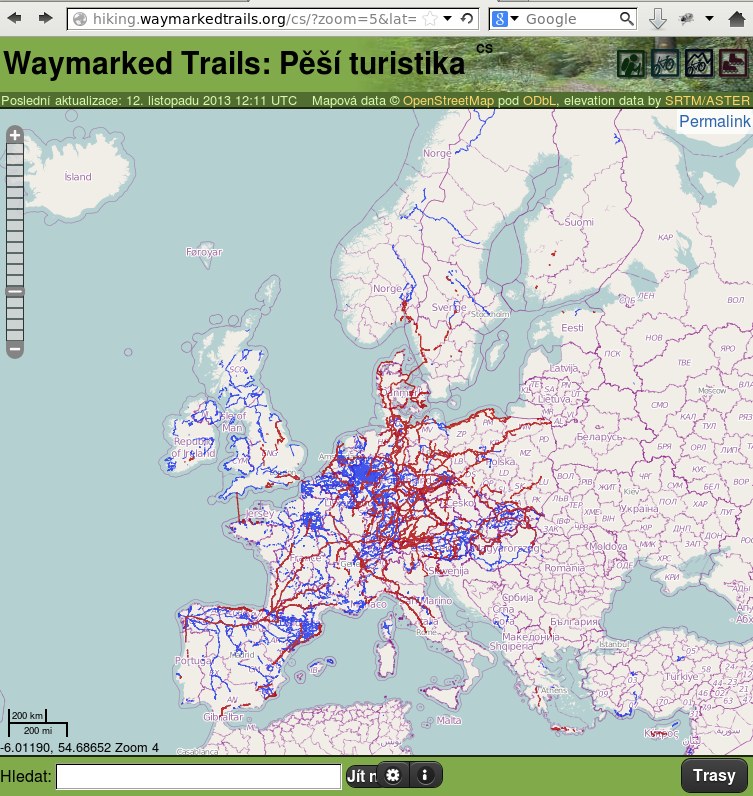
\includegraphics[width=8cm]{obrazky/waymarkedTrails.png}
				\caption{Hiking Map na Waymarked Trails}
				(zdroj: Waymarked Trails\cite{Waymarked})
			\end{center}
		\end{figure}
	
		\paragraph{} Velkou výhodou této mapy je poskytování informací o~trasách a možnost jejich uložení v~\ac{GPX} formátu. Trasy jsou rozděleny na:
	\begin{itemize}
		 \item kontinentální -- mezinárodní trasy vedoucí přes několik států, značené prefixem E
		 \item národní -- trasy \ac{kct}
		 \item regionální -- trasy \ac{kct}
     		 \item ostatní -- naučné stezky, odbočky k~hradům, zříceninám, vyhlídkám, přírodním zajímavostem apod.
	\end{itemize}
  Mapa také poskytuje možnost vyhledání místa podle názvu a vytvoření permanentního odkazu na mapový výřez. Mapa neposkytuje vyhledávání tras -- na to je potřeba použít jiná existující řešení, např. OpenRouteService (\url{http://www.openrouteservice.org/}), které kromě vyhledání trasy pro určitý typ dopravy (autem, na kole, pěšky) poskytuje i její export, výškový profil, vyhledání zájmových bodů v~blízkosti.

 	\section{OpenTrackMap}
		\url{http://opentrackmap.cz/}

                %%% ML: nerekl bych "ze odpada problem s licenci",
                %%% spise ze "licence ODBL umoznuje pouziti dat OSM
                %%% pro tyto typy aplikaci"
                
                %%% ML: chybi odkaz na Mapnik, slovo "zobrazeni" je v
                %%% teto souvislosti zavadejici

		\paragraph{} OpenTrackMap je projekt Ing. Radka Bartoně. Projekt běží na serveru geo102, který spravuje Katedra geomatiky na Fakultě stavební ČVUT v~Praze. Tvorba této aplikace byla motivována snahou poskytnout mapy pro aplikaci TangoGPS běžící na platformě Openmoko\cite{OTM}. Již existující mapy nemohly být z~licenčních důvodů či kvůli různým technickým omezením použity. Díky licenci \ac{ODbL} mohou být data \ac{OSM} použita. Data jsou uložena v~databázi PostgreSQL a pro jejich vykreslení je použit software Mapnik (\url{http://mapnik.org/}). Ačkoliv mapy v~současné době nejsou aktualizovány, jejich přínos je ve vytvoření značkového klíče pro tras a objektů v~mapě\cite{otm_klic}. 

		\begin{figure}[!h]
			\begin{center}
				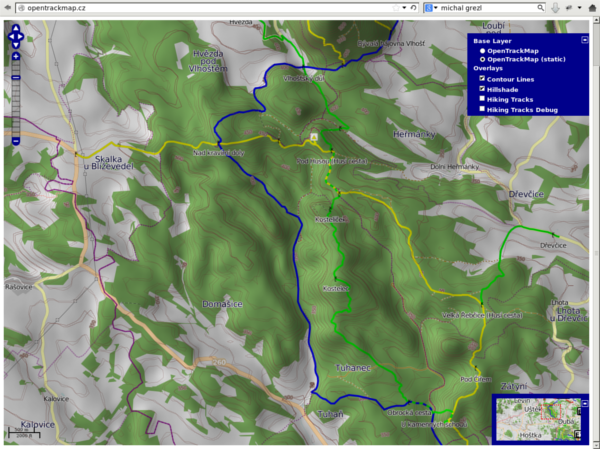
\includegraphics[width=12cm]{obrazky/otm.png}
				\caption{OpenTrackMap}
				(zdroj: \url{http://opentrackmap.cz})
			\end{center}
		\end{figure}

                %%% ML: chybi citace, odkud jste toto cerpal, v textu
                %%% vubec chybi odkazy na literaturu, clanky ze
                %%% kterych jste cerpal!!! zkuste jich par doplnit, to
                %%% je celkem ZASADNI nedostatek...

                %%% -> ML: v poradku, citaci jste doplnil v rozumne mire

		\paragraph{}  Aplikace poskytuje vrstevnice, stínování terénu, podkladovou mapu a turistické trasy. Vzhledem k~tomu, že mapy byly určeny pro zobrazení v~mobilních zařízeních, bylo zapotřebí snížit množství dat přenášených k~uživateli. Toho bylo dosaženo pomocí dlaždic. Původní testování odhalilo, že pro malá měřítka je vykreslování pomalejší, protože je pro velkou oblast vykreslováno stínování kopců\cite{OTM}. Od určitého stupně přiblížení se rychlost vykreslení mírně zvýšila, protože byla vykreslována menší plocha a protože klesl počet vektorových prvků.

	\section{MTB mapa Evropy}
		\label{sec:MTB}
		\url{http://mtbmap.cz/}
		\paragraph{} Projekt Martina Tesaře MTB mapa Evropy byl původně bakalářskou prací zpracovávanou na fakultě informatiky Masarykovy univerzity v~Brně. Aplikace prezentuje stezky pro jízdu na horském kole. Mapa byla původně omezena pouze na oblast České republiky a přilehlého okolí, ale časem byla rozšířena na celé území Evropy. Mapa využívá značkový klíč projektu OpenTrackMap, který je popsán na \ac{OSM} Wiki\cite{otm_klic}, a kromě cyklistických stezek zobrazuje i turistické cesty. Aktuálnost mapy je udržována týdenními aktualizacemi dat \ac{OSM}. Data pocházejí ze serveru \textit{geofabrik.de}, který poskytuje možnost stažení dat \ac{OSM} pro jednotlivé země, kontinenty i celý svět.

                %%% ML: prvni veta zni divne...

                %%% ML: co umoznuje sluzva Nominatim vyhledavat? v
                %%% dalsim textu to mate zmineno, ctenar musi ale
                %%% patrat

                %%% ML: co je editor iD, vysvetlit...

                %%% -> ML: OK

                %%% -> ML: zmenil jsem poradi obrazku, tak aby oba
                %%% nevychazeli na posledni stranku

		\begin{figure}[!h]
			\begin{center}
				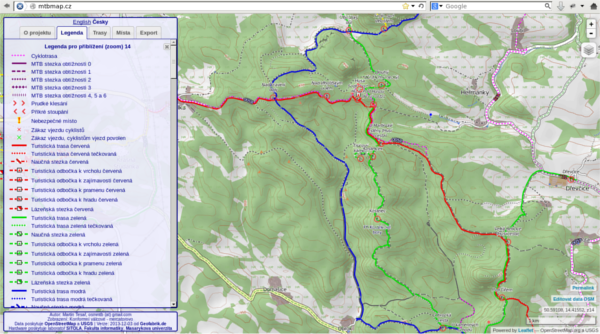
\includegraphics[width=12cm]{obrazky/mtb.png}
				\caption{MTB mapa Evropy}
				(zdroj: \url{http://mtbmap.cz/})
			\end{center}
		\end{figure}

		\paragraph{} Aplikace obsahuje řadu nástrojů. K~dispozici je vyhledávání pomocí služby \ac{OSM} Nominatim\cite{nominatim}. Tento nástroj slouží k~vyhledávání objektů pomocí jejich adresy. Dále lze exportovat data v~souřadnicemi daném výřezu. Zde lze nastavit stupeň přiblížení, velikost výsledku v~pixelech a zobrazené mapové prvky -- tiráž, název mapy, trasu, legendu a měřítko. Kromě vyhledávání míst  pomocí Nominatim je k~dispozici i vyhledání cesty podle množství vstupních parametrů, které zahrnují například typ cesty, druh povrchu nebo obtížnost. Tyto parametry jde uložit na disk a později je znovu použít pro vyhledání stejné cesty. Lze též vložit vlastní cestu v~souboru \ac{GPX} nebo ručně a zobrazit k~ní výškový profil. Takto vytvořené stezky se zobrazí v~mapě, ale neukládají se pro pozdější zobrazení. Aplikace umožňuje vygenerovat permanentní odkaz na zobrazenou pozici či přesměruje uživatele na web \acl{OSM} a otevře online editor dat \ac{OSM} iD.

                %%% ML: co je EPSG:3857 nejde jenom o kartograficke
                %%% zobrazeni, mluvil bych spise o souradnicovem
                %%% systemu

		\paragraph{} Tento projekt má svoji stránku na OpenStreetMap Wiki, kde jsou popsány úkoly, kterými by měl směřovat další vývoj aplikace. Mapa byla původně vytvořena v~OpenLayers\cite{tesar_bp}, ale v~současné době užívá javascriptovou knihovnu Leaflet. K~dispozici jsou 4 podkladové mapy (MTB mapa, OSM Mapnik, OpenCycleMap, Hike \& Bike Map), které jsou zobrazeny v~EPSG:3857. Tento souřadnicový systém je ekvivalentní s~EPSG:900913, které na svých mapách používá Google. Jak bylo uvedeno výše \ref{google_mercator}, toto zobrazení není přesně konformní, ovšem v~tiráži je uvedeno \uv{Zobrazení: Konformní válcové - Mercatorovo}, viz obr. \ref{fig:MTB_tiraz}.
		\begin{figure}[!h]
			\begin{center}
				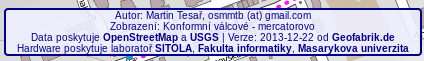
\includegraphics[width=8cm]{obrazky/tiraz.png}
				\caption{MTB mapa Evropy - tiráž}
				(zdroj: \url{http://mtbmap.cz/})
				\label{fig:MTB_tiraz}
			\end{center}
		\end{figure}

%%%%%%%%%%%%%%%%%%%%%%%
%%%%% OPEN STREET MAP        %%%%%
%%%%						      %%%%
%%%							  %%%
%%								     %%
%									 %
\chapter{OpenStreetMap}

		\paragraph{} Cílem této kapitoly je čtenáře seznámit s~projektem \acl{OSM}. Zmíněna bude jeho historie, současný stav a jeho využití.

	\section{O~Projektu}

        %%% ML: "a toto jméno se zde velice často objevuje" zni
        %%% opravdu spatne..., zduvodneni formulovane jako "Z toho
        %%% důvodu by bylo vhodné říci o co se jedná" je potreba
        %%% preformulovat, neco jako "cilem kapitoly je ...."

        %%% -> ML: OK (odstavec jsem presnul na zacatek kap

                %%% ML: "OpenStreetMap je svobodná mapa" je
                %%% zavadejici, nepresne a divne..., zkuste tuto cast
                %%% prepsat, opet chybejeji citace jako v celem textu...

                %%% ML: nejde o "mapove dilo" !!! jaka jina "mapova
                %%% dila" mate na mysli

                %%% ML: "stahnout si data" jaka data - neni vysvetleno

                %%% ML: OSM jiz nepouzivat CC-BY-SA !!! -
                %%% http://wiki.openstreetmap.org/wiki/Cs:ODbL/We_Are_Changing_The_License
                %%% opet chyby jakakoliv reference ... (!!!)

        %%% -> ML: OK
        
        %%% -> ML: mapova dila jsem zmenil na mapove aplikace

		\paragraph{} \acl{OSM} je mapa, kterou vytváří a spravují její uživatelé. Na rozdíl od jiných mapových aplikací\footnote{Např. Google Mapy.} \acl{OSM} poskytují uživatelům možnost stáhnout si data, která tvoří mapu, a v~rámci licence \ac{ODbL} s~nimi volně nakládat. Díky tomu vznikají různé mapové aplikace, která reflektují potřeby uživatelů (např. Waymarked Trails, viz kap. \ref{sec:waymarked}, nebo MTB mapa Evropy, viz kap. \ref{sec:MTB}). 
		\paragraph{}Projekt vznikl ve Velké Británii v~roce 2004. O~jeho základy se postaral Steve Coast, který se nechal inspirovat jiným, komunitou řízeným projektem -- svobodnou encyklopedií Wikipedie. O~dva roky později vznikla OpenStreetMap Foundation, která projekt podporuje. V~průběhu let povolily některé společnosti používat své mapové podklady pro tvorbu OpenStreetMap. V~roce 2006 to byl Yahoo. O~rok později Automotive Navigation Data poskytla mapy silniční sítě Nizozemska, Indie a Číny\cite{osm_wikipedia_en}.
		\paragraph{} Od vzniku aplikace vzrostl počet registrovaných uživatelů až na milion. V~srpnu 2008 měla aplikace 50 000 registrovaných uživatelů. Do konce násle\-dujícího roku narostlo toto číslo skoro na  200 000. V~roce 2012 služba registrovala 600 000 členů a 6. ledna 2013 překročil počet uživatelů 1 milion. Ze statistik vyplývá, že kolem 30\% uživatelů vytvořilo alespoň jednu sadu změn\cite{neis}.

                %%% ML: kazdy obrazek musi byt uveden zdroj !!!
                
                %%% ML: obrazek ma nevhodny popisek - uzivatelu ceho?
                %%% (je potreba uvest OSM), v seznamu obrazku to bude matouci

                %%% -> ML: OK

		\begin{figure}[!h]
			\begin{center}
				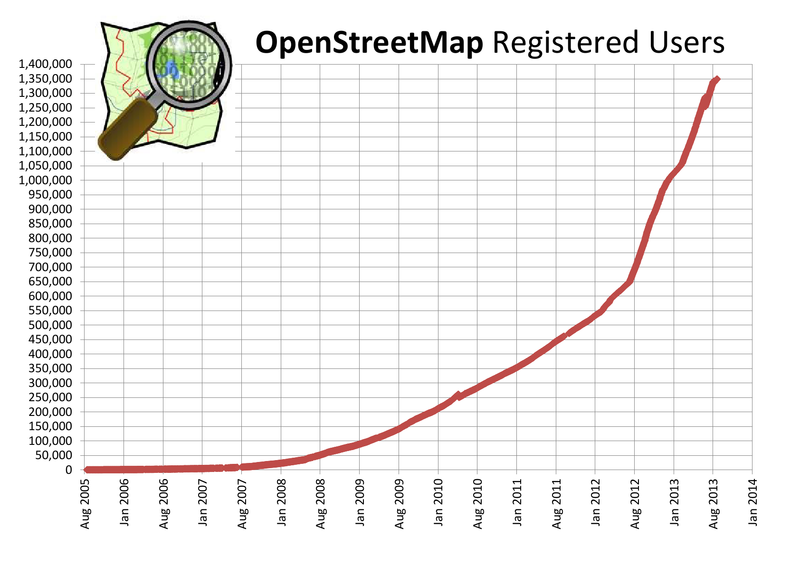
\includegraphics[width=12cm]{obrazky/osm_stat_users.png}
				\caption{Graf nárůstu registrovaných uživatelů \ac{OSM}}
				 (zdroj: \ac{OSM} wiki\cite{osm_wiki_stats})
			\end{center}
		\end{figure}

                %%% ML: jaka data? prilis obecne

                %%% -> ML: OK

	\section{Geodata}
		\subsection{Typy geografických dat}

                %%% ML: rozlicnych dat ci kvalitu dat, ci neco jineho
                %%% ??? nepresna formulace

                %%% ML: "standardnich objektu" to je velmi nepresne,
                %%% silnice ci vodstvo nejsou objekty...

                %%% ML: co mate na mysli "normalnimi mapami" ? je
                %%% treba to nejak rozvest...

                %%% ML: "Data mohou byt" zni divne, spise neco jako
                %%% "Rozlisuje tri zakladni elementy datoveho modelu,
                %%% ktery projekt OSM pouziva:" ci neco podobnebo

                %%% -> ML: OK

		\paragraph{} Jak už bylo řečeno, data pořizují samotní uživatelé mapy, což má za následek velkou druhovou rozmanitost dat. Kromě obvyklých prvků, jako jsou silnice, vodstvo, budovy, zalesněné oblasti či turistické značky, jsou mapovány i věci, které na jiných\footnote{Např. Mapy.cz či Google Mapy.} mapách zobrazeny nejsou. Jedná se například o~bezpečnostní kamery na veřejných místech. Datový model pracuje se třemi základními elementy:
	\begin{itemize}
		\item uzly (nodes) -- body se souřadnicemi,

                  %%% ML: nebo co?
                  %%% -> ML: OK

		\item cesty (ways) -- liniové prvky a hranice polygonů

                  %%% ML: jakymi dalsimi prvky?
                  %%% -> ML: OK

		\item relace (relations) -- popisují vztahy mezi jednotlivými prvky.
	\end{itemize}
Kromě těchto tří elementů mohou mít prvky své tagy, do kterých se zaznamenávají  vlastnosti. 	

%%% ML: "nebo jsou součástí cesty" zni divne, mate na mysli, ze uzly
%%% tvori lomove body cesty? nebo jenom pocatecni a koncovy bod cesty
%%% (lomene cary) ?

%%% -> ML: OK

		\paragraph{}Uzly mají přiřazeny zeměpisné souřadnice a identifikátor (id). Volitelně může být prvku přiřazena i výška. Uzly mohou být samostatné prvky (např. rozcestník či sloup) nebo jsou lomovými či koncovými body cesty. V~tom případě definují její tvar. Uzly musí být na spojnicích více cest -- např. když se protínají dvě cesty, tak součástí obou cest musí být stejný vrchol. Pokud by to tak nebylo, nejednalo by se z~topologického hlediska o~křižovatku, ale o~mimoúrovňové křížení. Globální dataset obsahuje k~roku 2013 přes 2 x 10$^9$ uzlů\cite{osm_wiki_node}.

%%% ML: chybi zdroj, to musite uvest...

%%% -> ML: OK

		\begin{figure}[!h]
			\begin{center}
				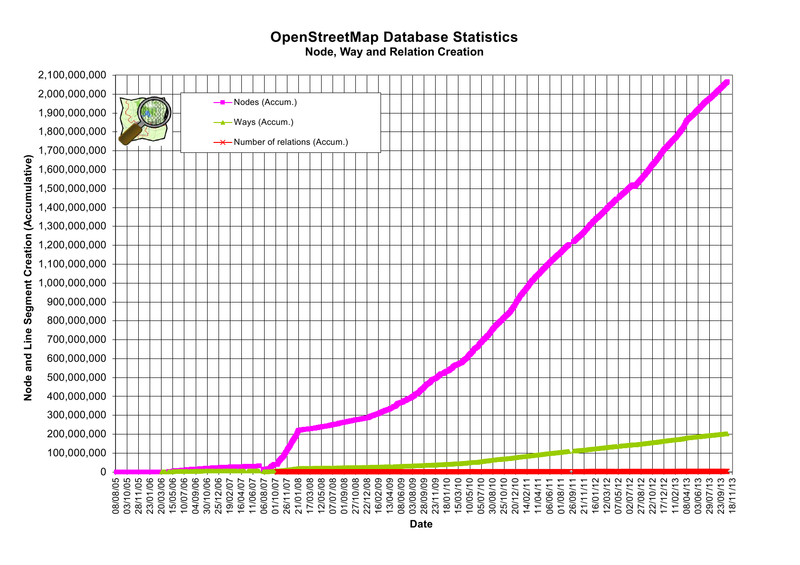
\includegraphics[width=12cm]{obrazky/osm_stat_elements.png}
				\caption{Graf vývoje počtu uzlů, cest a relací}(zdroj: \ac{OSM} wiki\cite{osm_wiki_stats})
				\label{fig:elements}
			\end{center}
		\end{figure}

                %%% ML: "Oproti uzlům je cest výrazně míň" to nezni
                %%% prilis staste, zkuste preformulovat, jedna se o
                %%% text technickeho charakteru

                %%% -> ML: OK (doplil jsem jeste uvozovky u area a yes)

		\paragraph{} Cesty jsou tvořeny 2 až 2000 uzly spojenými liniovými segmenty. Z~grafu na obr. \ref{fig:elements} je vidět, že v~databázi je ke konci roku 2013 přes 200 000 000 cest.  Cesta je buď otevřená, nebo uzavřená. Otevřená cesta je taková, kde začátek a konec tvoří jiný uzel. Uzavřená cesta má identický počáteční a koncový uzel. V~tomto případě se může jednat o~uzavřenou polylinii či plošný prvek. Rozdíl lze stanovit pomocí tagu \uv{area} -- pokud má hodnotu \uv{yes}, jedná se o~plochu. V~některých případech může cesta tvořit polylinii a hranici polygonu zároveň -- toto je pak označeno odpovídajícím způsobem ve vlastnostech.

		\begin{figure}[!h]
			\begin{center}
				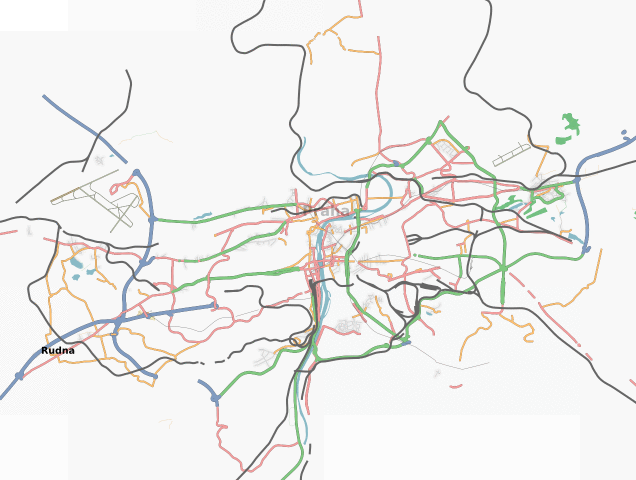
\includegraphics[width=12cm]{obrazky/Osm-200607-praha.png}
				\caption{Praha na mapách \ac{OSM} -- červenec 2006} (zdroj: Wikipedie\cite{osm_wikipedia_cs})
				\label{fig:praha2006}
			\end{center}
		\end{figure}

                %%% ML: "Vznik dat" divne, zkuste preformulovat - zdroje dat

                %%% ML: "chodi venku" nezni jako formulace s diplomove prace

                %%% ML: "souradnice, ktere pak importuje v souboru GPX
                %%% do mapy" zni opet divne, tuto formulace by me
                %%% neprekvapila jinde, ale u zaverecne prace oboru
                %%% "geoinfomatika" ano, zkuste prepsat

                %%% ML: Druhou "variantou" jako variantou, dalsim zdrojem dat ....

                %%% -> ML: OK

		\paragraph{} Data ukládaná do databáze \acl{OSM} mohou vzniknout třemi ce\-stami. První z~nich je přímý sběr v~terénu, kdy uživatel pomocí GPS přístroje získává souřadnice, které pak ve formátu \ac{GPX} nahraje do databáze. Dalším zdrojem dat je odvozování z~existujících mapových děl. Zde je ovšem potřeba dávat pozor, aby podklady pro odvození  byly kompatibilní s~licencí, kterou užívá \ac{OSM}. V~případě, že nejsou vyjasněny licenční podmínky, materiály použity být nemohou. Pro odvozování na území České republiky se dá kupříkladu použít ortofoto poskytované přes \ac{WMS} \ac{uhul} či \ac{WMS} katastrální mapy \ac{cuzk}\cite{freemap}. \ac{WMS} ortofotomapy \ac{cuzk} se jako zdroj použít nemůže, ale dá se s~ní ověřit přesnosti jiných zdrojů. Třetí možným zdrojem dat jsou komerční firmy, které poskytnou svá geodata k~dispozici.

                %%% ML: opet chybi zdroj

                %%% -> ML: OK

		\begin{figure}[!h]
			\begin{center}
				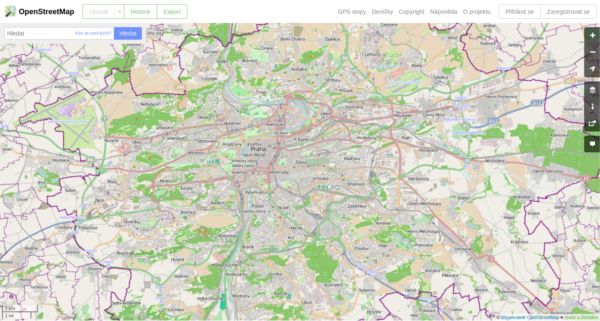
\includegraphics[width=12cm]{obrazky/Osm-201312-praha.png}
				\caption{Praha na mapách \ac{OSM} -- prosinec 2013}(zdroj: \ac{OSM}\cite{osm_wikipedia_cs})
				\label{fig:praha2013}
			\end{center}
		\end{figure}


                %%% ML: chybi odkaz na graf, ctenar musi hledat...

                %%% ML: konec odstavce: "zatímco druhý obrázek je
                %%% plnohodnotnou mapou." je spatna formulace, obrazek
                %%% muze byt tezkou mapou, 

                %%% -> ML: OK

		\paragraph{} Graf vývoje počtu elementů \ref{fig:elements} ukazuje, že z~počátku přibývalo malé množství objektů a větší zvrat nastal spolu s~nárůstem počtu uživatelů. V~roce 2007 je vidět skokový narůst počtu bodových prvků -- jedná se o~data silniční sítě Nizozemska, Indie a Číny poskytnuté organizací Automotive Navigation Data. 
		Přibývání počtu prvků v~mapě lze též dobře sledovat na malých plochách. Pro ilustraci jsou zde přiloženy obrázky, jak Praha byla zmapována v~roce 2006 \ref{fig:praha2006} a v~prosinci 2013 \ref{fig:praha2013}. V~prvním případě jsou zmapovány hlavní silnice a vodní toky, zatímco druhý obrázek zobrazuje mapu srovnatelnou s~mapou Prahy, kterou poskytují Mapy.cz nebo Google Mapy.
	
	\subsection{Uložení dat}
		\paragraph{} Data se ukládají do databáze, která je klíčovým prvkem celého projektu. Pro každý typ prvku existují tabulky v~databázi. Kromě současné verze obsahuje databáze i historické verze, takže lze dohledat změny a případně je vrátit. Další tabulky se vztahují ke změnovým sadám (changesetům), GPX souborům nebo registrovaným uživatelům. Kromě tabulek jsou uloženy i primární a cizí klíče, sekvence a indexy.

                %%% ML: "extrakt" neni rozhodne ceske slovo... zkuste
                %%% najit lepsi termin, dale pouzivate "vytahy" coz
                %%% neni take uplne stastny termin

                %%% -> ML: OK

		\paragraph{} Data jsou distribuována v~XML souboru Planet.osm, který je vytvářen v~týdenních intervalech. V~současnosti je velikost nekomprimované sady přes 400 GB, při užití komprimace je možno se dostat k~29 GB. Protože dost často není potřeba mít data z~celého světa, dělají se i výběry, které pokrývají jednotlivé kontinenty, země nebo města. Tyto soubory jsou vytvářeny častěji -- \url{http://download.geofabrik.de} poskytuje data s~denním intervalem. Vytvoření obrazu databáze většinou zabere 12 hodin\cite{planet.osm}.

                %%% ML: "mapova data" co to je? co je format GPX,
                %%% nikde neni vystetleno

                %%% -> ML: OK

	\paragraph{} Kromě dat tvořících mapu jsou k~dispozici i planet.gpx s~údaji z~nahraných \ac{GPX}\footnote{\ac{GPX} je výměnný formát založený na \ac{XML} pro data z~GPS přijímačů.} souborů a soubor s~historií, který obsahuje každou revizi každého objektu. Planet.gpx obsahuje v~nekomprimovaném stavu 55 GB dat, historie změn kolem 500 GB\cite{osm_wiki_planet.gpx}. 

        %%% ML: odkud tyto informace jsou, jako vsude v textu CHYBI
        %%% REFERENCE!!!

        %%% -> ML: OK

	\paragraph{} Data jsou uložena na databázovém serveru, který má dostatečné prostředky pro správu těchto dat. Od dubna 2009 do dubna 2012 byl primárním serverem server Smaug\cite{osm_wiki_smaug}. Operační systém Ubuntu 12.04 LTS Server amd64 obsluhuje relační databázi PostgreSQL ve verzi 9.1. Pevné disky mají kapacitu přes 6 TB a operační paměť je 64 GB. V~současné době je primárním serverem server se jménem Ramoth\cite{osm_wiki_ramoth}, který je také obsluhován operačním systémem Ubuntu 12.04 LTS Server amd64, ovšem od svého kolegy se liší jak kapacitou disků (skoro 15 TB), tak operační pamětí (256 GB). Funkci databázového systému plní stále PostgreSQL 9.1.

        %%% ML: asi mate na mysli popisna data, vlastnosti jsou
        %%% zavadejici

        %%% -> ML: OK

	\paragraph{}Každý záznam v~databázi má u~sebe uvedena popisná data. Protože pro každý typ prvku je jedna tabulka, jsou některé sloupce s~popisnými daty prvku prázdné. Parametry, které se evidují např. u~silnice, jsou jiné než parametry, které nás zajímají u~řeky -- obojí lze najít v~tabulce s~liniovými prvky. Aby se běžný uživatel či vývojář vyznali v~databázi, jsou vytvořeny na wiki projektu stránky, které popisují všechna popisná data (sloupce v~databázi) a hodnoty, kterých můžou nabývat. Díky tomu je hledání v~databázi vůbec možné a~nepřipomíná hledání v~jehly v~kupce sena.


	\section{OSM editory} % id, Potlach 2, JOSM, Merkaator
		\label{sec:editory}
		\paragraph{} Součástí předkládané diplomové práce je napojení editoru vytvářené web\-ové aplikace na data \ac{OSM}. Stojí tedy za zmínku, jaké jsou prostředky, kterými se v~současné době provádí editace dat projektu \ac{OSM}. 
		\subsection{iD}

                %%% ML: chybi odkaz na d3js, co znamena "práci v datech založených dokumentech" ?

                %%% ML: jako nikde v textu nejsou vysvetleny zkratky -  HTML, CSS a dalsi

                %%% -> ML: OK

			\paragraph{}Editor iD je nejnovějším z~uvedených editorů. Pro užití na OpenStreetMap byl spuštěn v~květnu 2013. Jedná se o~javascriptovou aplikaci, která je šířena pod licencí \ac{WTFPL}\cite{wiki_wtfpl}, která umožňuje naprosto volně nakládat s~produktem. K~vykreslení je užívána javascriptová knihovna d3js\footnote{\url{http://d3js.org/}}, která slouží k~práci v~datech založených dokumentech. Knihovna užívá \ac{HTML}, \ac{CSS} a \ac{SVG} k~vykreslení požadovaných prvků. Podpora jiných vykreslovacích přístupů není zatím v~editoru iD implementována. Jedná se o~aplikaci vhodnou pro začátečníky, protože má jednoduché ovládání.

		\begin{figure}[!h]
			\begin{center}
				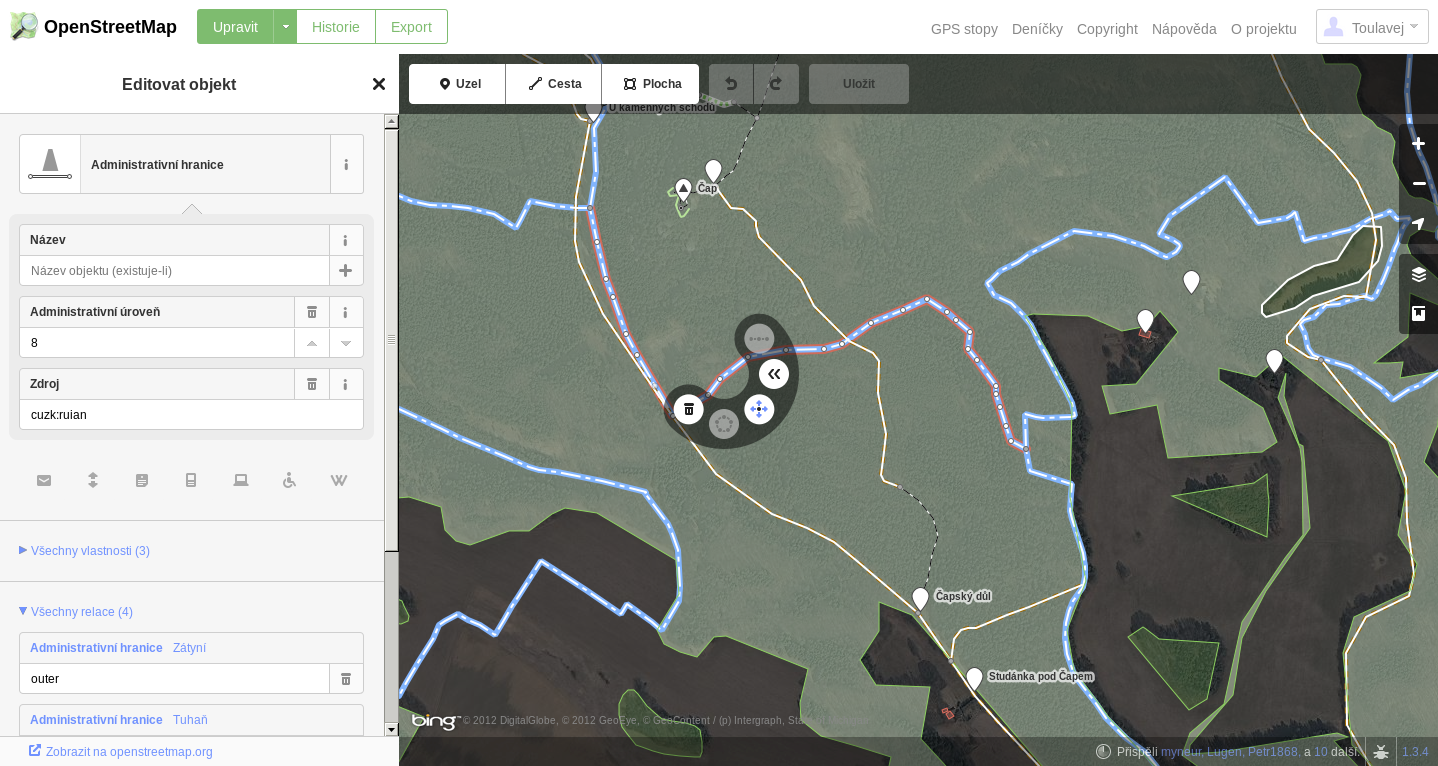
\includegraphics[width=12cm]{obrazky/iD_osm.png}
				\caption{Editor iD na webu OpenStreetMap.org} (zdroj: \ac{OSM}\cite{osm_edit})
				\label{fig:iD_osm}
			\end{center}
		\end{figure}

			\paragraph{} Podle stránek projektu\cite{wiki_iD} program zatím plně nepodporuje prohlížeče Internet Explorer verze 9, 10 a 11. Někteří uživatelé též hlásili zhoršený výkon pro prohlížeč Firefox.

		\subsection{JOSM}
			\paragraph{}\ac{JOSM}je na Javě založený editor dat \ac{OSM}. Jedná se o~desktopovou aplikaci publikovanou pod licencí \ac{GPL}, ze které jsou změny dálkově nahrávány do hlavní databáze \ac{OSM}\cite{wiki_josm}. Na rozdíl od iD poskytuje JOSM mnohem více možností pro manipulaci s~daty\cite{wiki_comparison}, což je znát i na jeho uživatelském rozhraní, viz obr. \ref{fig:josm_osm}. Aplikace podporuje čtení \ac{GPX} souborů buď z~pevného disku nebo z~databáze\acl{OSM}, editování existujících uzlů, cest, tagů a relací.

                        %%% ML: jediny obrazek se zdrojem, no konecne :-)

		\begin{figure}[!h]
			\begin{center}
				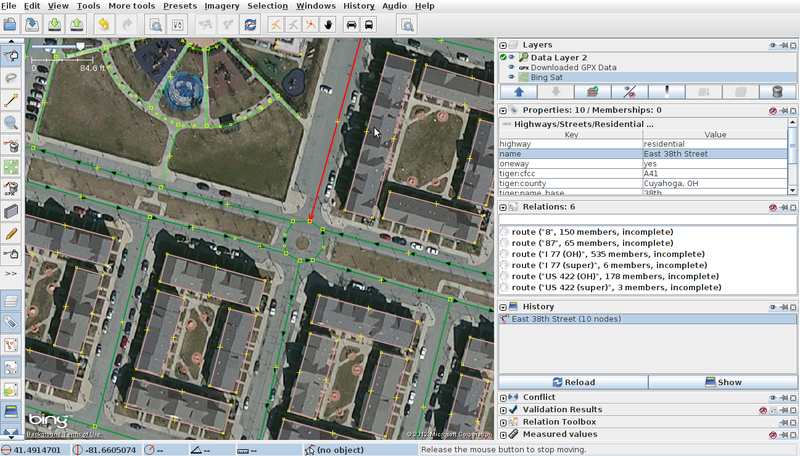
\includegraphics[width=12.6cm]{obrazky/josm_osm.png}
				\caption{Editor JOSM} (zdroj: OSM Wiki\cite{wiki_josm})
				\label{fig:josm_osm}
			\end{center}
		\end{figure}
			\paragraph{} Výhodou oproti online editorům je možnost pracovat i bez připojení k~internetu. Aplikace také poskytuje různá rozšíření, která z~ní dělají velmi silný editovací nástroj. Dle informací na OpenStreetMap Wiki\cite{wiki_josm} je práce s~tímto editorem jednoduchá. Některé pokročilejší funkce mohou mít složitější ovlá\-dání a jejich zvládnutí může zabrat čas.

		\subsection{Merkaator}
			\paragraph{} Editor Merkaator je určen pro Unix, Mac OS i Windows a je distribuován pod licencí GNU \ac{GPL} v2. Editor je ve stádiu vývoje (dle OpenStreetMap Wiki je dostupná verze 0.18.1 vydaná v~červnu 2012), ovšem vývojářská komunita tohoto projektu není příliš aktivní\cite{wiki_merkaator}. Aplikace obsahuje prvky, které stojí za povšimnutí. Jedná se například o~průhledné zobrazení vrstev, editor stylů zobrazení mapy, přímé připojení k~GPS přijímači nebo vykreslení mapy do \ac{SVG} nebo bitmapového obrázku za použití momentálně užitých stylů. Vzhledem k~tomu, že je program ve vývoji, lze některé prvky získat pouze kompilací ze zdrojových souborů, což pro většinu uživatelů není vhodné.

		\begin{figure}[!h]
			\begin{center}
				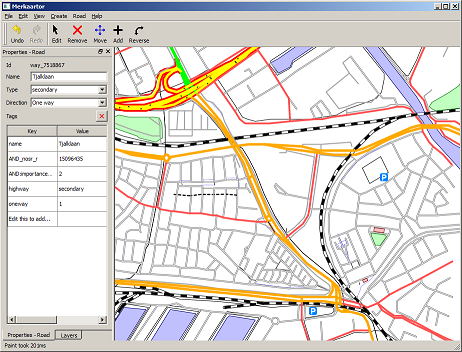
\includegraphics[width=10.5cm]{obrazky/merkaator_osm.png}
				\caption{Editor Merkaator} (zdroj: OSM Wiki\cite{wiki_merkaator})
			\end{center}
		\end{figure}

		\subsection{Potlatch 2}
			\paragraph{} Stejně jako iD editor je i Potlatch 2 online editor s~licencí \ac{WTFPL}, ale na rozdíl od něj je napsán ve Adobe Flash. Jedná se o~jednoduchý editor, který není určen pro náročnější uživatele. Potlatch 2 vznikl kompletním přepsáním původního Potlatch\cite{wiki_p2}, kdy byly přidáno zobrazení \ac{WYSIWYG}, jednodušší tagování a autentizace přes OAuth pro zakomponování do jiných stránek při zachování napojení na OpenStreetMap. Z~důvodu existence editoru iD není v~současnosti aplikace aktivně vyvíjena.

                        %%% ML: zdroj nelze dohledat

                        %%% -> ML: OK

                        %%% -> ML: zmensil jsem obrazky tak aby se
                        %%% vesly na jednu stranku a zbytecne text
                        %%% nedrobily
                        
		\begin{figure}[!h]
			\begin{center}
				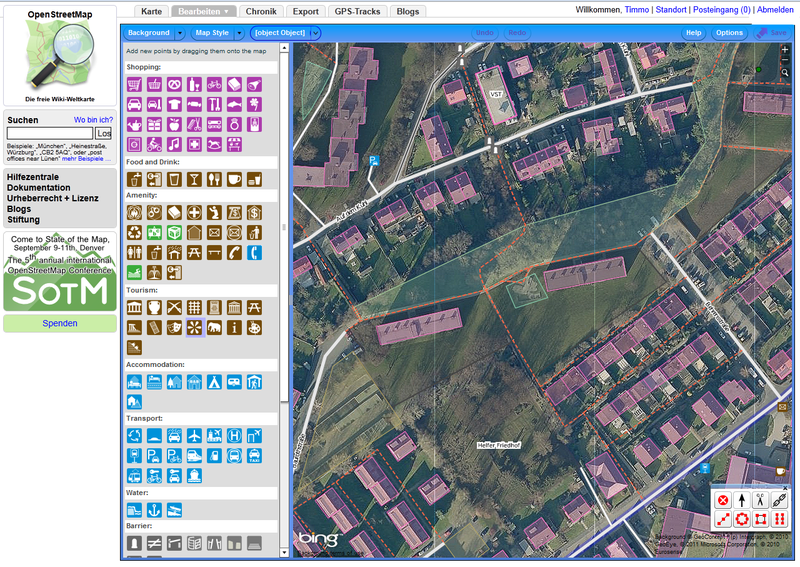
\includegraphics[width=10.5cm]{obrazky/p2_osm.png}
				\caption{Editor Potlatch 2}(zdroj: OSM Wiki\cite{wiki_p2})
			\end{center}
		\end{figure}

	\section{Využití dat \ac{OSM}}
		\paragraph{} Data \ac{OSM} jsou často využívána k~tvorbě tématických map, např. z~oblasti turistiky. Mapy mohou též sloužit jako podklady do navigací. Řada velkých projektů, např. Foursquare, užívá nebo přechází na mapy OpenStreetMap, protože jsou pro ně výhodnější. Ačkoliv tyto produkty ocení většina uživatelů, dle mého názoru leží větší význam map OpenStreetMap v~oblasti humanitární pomoci.
		\paragraph{}V momentě, kdy nějakou část světa zasáhne živelná katastrofa, mohou dobrovolníci z~řad uživatelů OpenStreetMap z~aktuálních družicových snímků vytvořit novou aktuální mapu postižené oblasti. Toto bylo využito třeba v~roce 2010, kdy bylo Haiti zasaženo zemětřesením, a v~současnosti probíhá nové mapování po tajfunu na Filipínách z~listopadu 2013. Během prvního týdne od tajfunu bylo editováno víc jak 2~000~000 objektů a do obnovy se zapojilo přes 900 uživatelů. K~11.prosinci 2013 bylo za přispění více jak 1~600 uživatelů zmapováno přes 4,5 milionu objektů\cite{wiki_tajfun}.
		\paragraph{} Aby byla zajištěna efektivní tvorba, produkce a distribuce map pro postižené oblasti, byla v~lednu 2009 vytvořena skupina Humanitarian OpenStreetMap Team\cite{wiki_hot}, která tuto činnost řídí.
	

%%%%%%%%%%%%%%%%%%%%%%%
%%%%% POUŽITÉ TECHNOLOGIE%%%%%
%%%%						      %%%%
%%%							  %%%
%%								     %%
%									 %
\chapter{Použité technologie}

%%%Servery
	\section{Apache HTTP Server}

        %%% ML: v tomto textu michate dohromady specializovany
        %%% software "webovy server" s obecneji vmimanym pojmem
        %%% "server", zkuste tento odstavec prepsat

        %%% -> ML: OK (poznamky pod carou tady vypadaji divne, ale
        %%% nechte to byt (pouze muj subjektivni dojem)

		\paragraph{}\label{sec:server} V~souvislosti s~webovými aplikacemi se objevuje pojem server, který může odkazovat buď na hardware\footnote{Tj. počítač.}, který poskytuje nějaké služby, nebo na software\footnote{Tj. program.}, který tyto služby realizuje, např Apache HTTP Server nebo Geoserver. Aplikace, které se k~serveru připojují a požadují poskytované služby, se nazývají klienti\label{sec:klient}. Tím je např. webový prohlížeč.
		\paragraph{} Při výběru webového serveru je možné si vybrat z~několika aplikací. Nej\-častěji užívaným je Apache HTTP Server, viz kap. \ref{sec:marketShare}, poté je IIS od Microsoftu, nginx od NGINX, Inc. a GWS od Googlu. Protože při vývoji aplikace byl použit server Apache HTTP Server, budou následující řádky věnovány jemu.
		\begin{figure}[!h]
			\begin{center}
				
\includegraphics[width=5cm]{obrazky/apacheLogo.png}
				\caption{Logo projektu Apache HTTP Server}
				(zdroj: Wikipedie -- Apache HTTP Server\cite{wiki-Apache})
			\end{center}
		\end{figure}

                %%% ML: "z webove stranky" - mate na mysli "klienta" -
                %%% potom chybi vysvetleni pojmu "server" a "klient"
                %%% (viz odstavec vyse)

                %%% -> ML: OK

		\paragraph{} Apache HTTP Server častěji bývá označován pouze jako Apache. Jeho funkce spočívá v~přijímání požadavků od klienta, kterým je webový prohlížeč. Následně je zpracuje a zašle klientovi odpověď. Zpracováním se rozumí např. odeslání statické webové stránky nebo předání požadavku dalším aplikacím. Samotná komunikace je zajištěna přes \ac{HTTP}, který slouží pro přenos hypermedií\cite{rfc2616},např. \ac{HTML} stránek.
		\paragraph{}Apache má velké množství modulů, které mohou a nemusí být spuštěny. Pokud jsou zapnuty, rozšiřují možnosti samotného jádra. Při vývoji aplikací je ovšem potřeba, aby na vývojovém a produkčním serveru byly povoleny stejné moduly. V~opačném případě může docházet k~problémům s~funkčností. Běžně užívané moduly jsou např. mod\_rewrite, který slouží k~přepisování URL adresy, mod\_php přidávající Apachi podporu pro zpracování PHP skriptů nebo mod\_ssl pro šifrovaná spojení. Ve srovnání s~celkovým počtem modulů je toto jen velmi malý vzorek.

                %%% ML: CHYBI zdroj tohoto tvrzeni, musite ho doplnit,
                %%% jinak je to jenom vykrik do tmy

                %%% -> ML: OK

		\paragraph{}\label{sec:marketShare} Apache je nejrozšířenější webový server -- dle odhadů\cite{netcraft_survey} z~června 2013 obsluhovaly servery s~Apachem 54,2\% všech aktivních webových stránek a~53,3\% všech stránek. Toto postavení je pravděpodobně způsobeno několika faktory:
		\begin{itemize}
			\item užití Apache License, která umožňuje svobodné užívání softwaru,
			\item veřejně přístupné zdrojové kódy,
			\item rychlost je srovnatelná s~komerčními servery a 
			\item podpora všech hlavních operačních systémů.
		\end{itemize}
		
                %%% ML: open chybi zdroj !!!

                %%% -> ML: OK

		\begin{figure}[!h]
			\begin{center}
				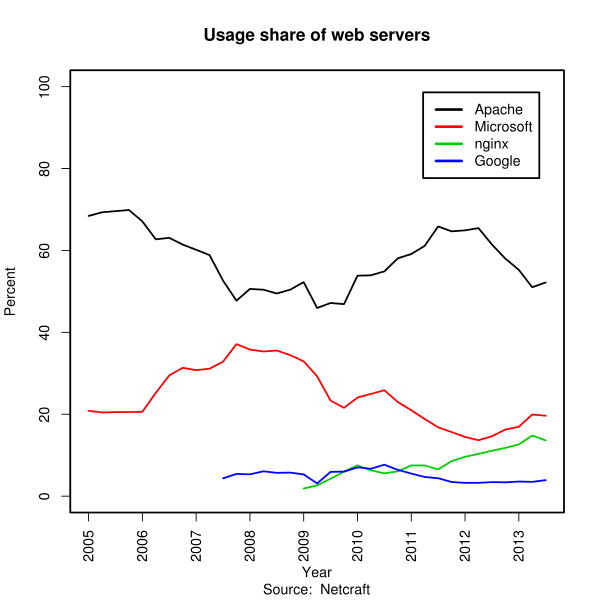
\includegraphics[width=6cm]{obrazky/servers_share.png}
				\caption{Zastoupení jednotlivých serverů}
				(zdroj: Wikipedia -- Web server\cite{wiki_webServer})
			\end{center}
		\end{figure}

		\paragraph{} Důvodem pro užití Apache byly přednosti vyjmenované výše -- zejména rychlost a to, že se jedná o~svobodný software. Jeho nastavení se sice provádí pomocí textového editoru, to ovšem není taková překážka, protože webové stránky projektu poskytují dostatečnou dokumentaci a v~případě problémů není složité dohledat řešení na internetových fórech věnovaných právě serverům. Jedním z~důvodů, pro tuto volbu byl fakt, že na školním serveru geo102 je nainstalován právě Apache.

	\section{Geoserver}
		\paragraph{} V~předchozí části bylo uvedeno, že webový server může přesměrovat některé dotazy jiným aplikacím. Dotazy na prostorové informace lze přesměrovat na mapový server. Pokud se pohybujeme v~rovině svobodného softwaru, existují dvě možnosti -- Geoserver a UMN MapServer. V~komerční sféře lze najít servery od firem Esri, Intergraph a dalších. 

                %%% ML: chybi zdroj

                %%% -> ML: OK

		\begin{figure}[!h]
			\begin{center}
				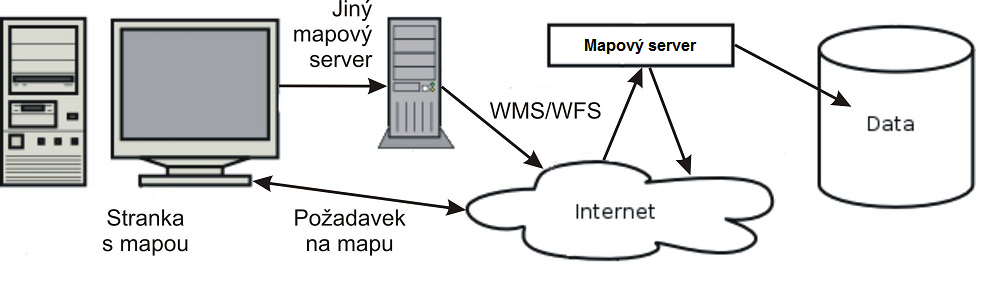
\includegraphics[width=10cm]{obrazky/mapserver.png}
				\caption{Schéma funkce mapového serveru}
				\label{fig:server_schema}
				(zdroj: Jan Doležal - diplomová práce\cite{dp_dolezal} (upraven))
			\end{center}
		\end{figure}
Mapový server podle určitých pravidel vygeneruje obraz požadovaného výřezu mapy, který odešle webovému serveru. Ten ho pak odešle zpátky uživateli. Pravidla pro generování jsou dána parametry, které může a nemusí uživatel zadat. Mezi parametry lze třeba najít požadovaný výstupní formát.

               %%% ML: nejlepsi, proc? tato formulace zavani "flame-war"

               %%% ML: nekomercni? proc? naopak je to vcelku komercne
               %%% vyuzitelne reseni, jiz opraveno na "open source"

               %%% ML: minimalne WMS zkratku by bylo dobre rozepsat...

%%% -> ML: OK (mnohem lepsi)

		\paragraph{} Geoserver je open source řešení s~podporou všech běžně užívaných webo\-vých služeb. Aplikace podporuje velké množství vstupních a výstupních formátů. Vstupem může být například PostGIS databáze, Esri Shapefile, GeoTIFF či \ac{WMS} služba. Výstup může být například ve formátu PNG, PDF, JPEG, KML, CSV nebo JSON.  Geoserver je napsán v~Javě a pro jeho nastavení a správu se používá webové rozhraní, které je normálně dostupné na portu 8080, ale tento port může být změněn. Zde lze nastavit poskytované vrstvy a služby. Správa uživatelů a uživatelských rolí se provádí také zde. 
		\begin{figure}[!h]
			\begin{center}
				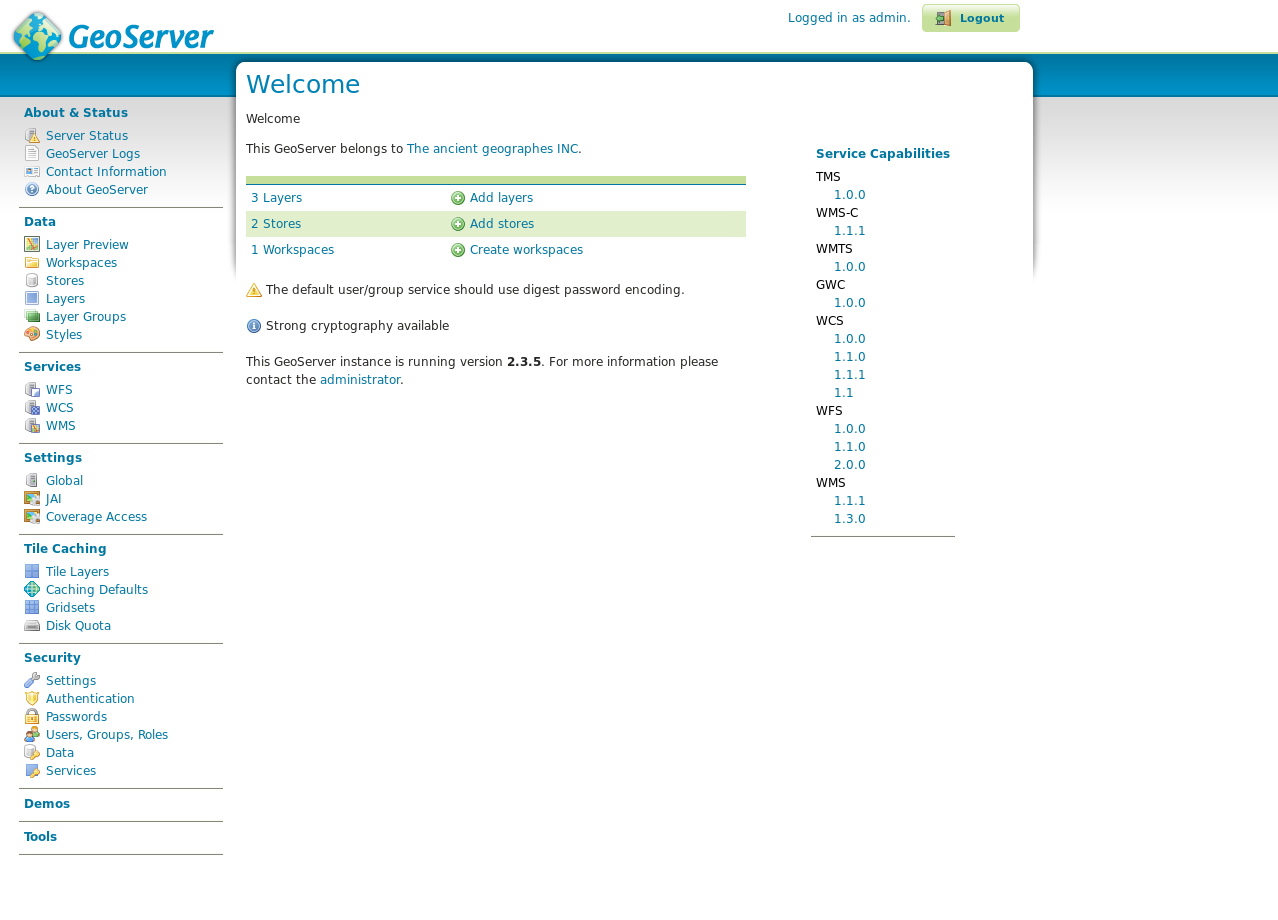
\includegraphics[width=10cm]{obrazky/geoserver.png}
				\caption{Uživatelské rozhraní Geoserveru}
				(zdroj: snímek obrazovky)
			\end{center}
		\end{figure}

                %%% ML: "Jedná se typ XML (eXtended Markup Language)."
                %%% neexistuje "typ" xml, SDL je odvozen ci zalozen na
                %%% XML

                %%% -> ML: OK

		\paragraph{}Pro nastavení vzhledu publikovaných vrstev se používá \ac{SLD} schéma, které je založeno na  \ac{XML}. Pravidla lze zapsat do textového pole, což vyžaduje určité zkušenosti s~tímto formátem. Geoserver ale také poskytuje možnost importovat pravidla  vytvořená v~jiném programu. Takto lze úspěšně použít Quantum GIS\cite{qgis} či AtlasStyler\cite{atlas} pro tvorbu vzhledu prvků.

                %%% ML: co je WMS-T a proc to bude potreba, vysvetlit
                %%% ci uvest odkaz na kapitolu, kde to bude vysvetleno

                %%% ML: proc nemohl byt pouzit MapServer, vysvetlit

                %%% -> ML: OK

		\paragraph{} Výběr Geoserveru byl dán zejména snahou využít svobodný software. Před začátkem tvorby se předpokládalo, že aplikace bude potřebovat zejména pro editaci dat \ac{OSM} službu \ac{WFS-T}, která umožňuje data upravovat a následně ukládat. MapServer nemá podporu \ac{WFS-T} a z~tohoto důvodu nemohl být použit. Výhodou Geoserveru je uživatelské rozhraní pro nastavení a publikování vrstev, protože MapServer se nastavuje pomocí konfiguračních souborů.

%%%Databáze
	\section{PostgreSQL}

        %%% ML: "bere data" - to snad ne ;-) PREPISTE TO

        %%% ML: samotny soubor? neco jako souborove orientovany format
        %%% jako napr. Esri Shapefile

        %%% ML: vyuziti jednotlivych souboru? jakych ?


        %%% ML: "PostgreSQL nabízí širší škálu funkcí" --- nezminujete
        %%% se vubec o PostGISu, aha, je zminka v dalsim odstavci

        %%% -> ML: OK

		\paragraph{} Na obrázku \ref{fig:server_schema} je zobrazeno, že mapový server přistupuje k~datům, která jsou uložena buď v~samostatném souboru, např. Esri Shapefile, nebo v~databázi. Pro potřeby webových aplikací se spíše užívají databáze, ačkoliv využití jednotlivých souborů s~geodaty také není vyloučeno. Mnoho webových aplikací používá relační databázi MySQL, ale z~hlediska vhodnosti pro tuto aplikaci byla zvolena jiná relační databáze -- PostgreSQL. Ačkoliv MySQL má podporu pro prostorová data, PostgreSQL nabízí širší škálu funkcí, viz kap. \ref{par:rozsireni}. Navíc existují pro PostgreSQL programy, které usnadňují import dat \ac{OSM}. V~neposlední řadě k~této volbě přispěl i fakt, že projekt \ac{OSM} používá PostgreSQL.
		\begin{figure}[!h]
			\begin{center}
				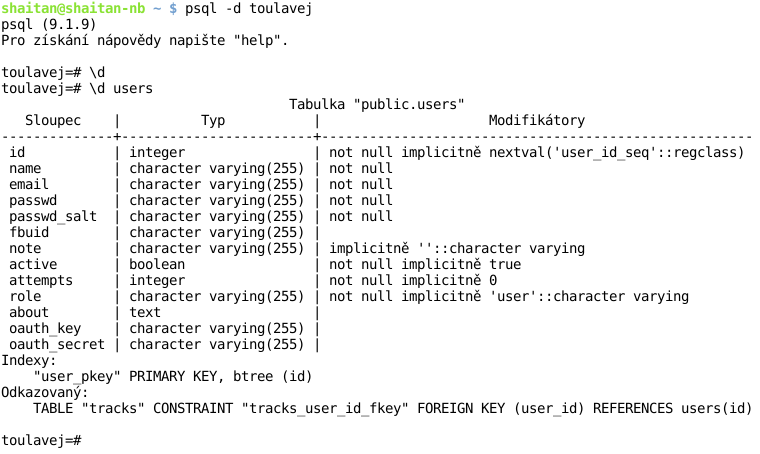
\includegraphics[width=10cm]{obrazky/psql.png}
				\caption{Terminál s~aplikací psql}
				\label{fig:psql}
				(zdroj: snímek obrazovky)
			\end{center}
		\end{figure}


                %%% ML: nezapomente na kontrolu pravopisu, na rade
                %%% mist jsem opravil chyby jako "standart" a dalsi

                %%% ML: "hashích" ??? to neni odborny termin

                %%% -> ML: OK

		\paragraph{}PostgreSQL je databázový systém napsaný v~jazyce C. Kromě Linuxu je možné s~ním pracovat i na počítačích s~operačními systémy Windows, Mac OS X, Solaris aj. PostgreSQL je licencován pod PostgreSQL License, která je podobná licenci MIT.  Implementace SQL v~PostgreSQL  odpovídá standardu ANSI--SQL:2008\cite{PostgreSQL} a také obsahuje většinu ze standardu SQL:2011\cite{wiki_postgresql}. Systém podporuje použití primárních (PRIMARY) a cizích klíčů (FOREIGN KEYS), triggerů, podmínek UNIQUE a NOT NULL. Indexy mohou být uloženy v~B-stromech, R-stromech, hashovacích tabulkách nebo GiST (Generalized search tree) vyhledávacích stromech. Současná stabilní verze PostgreSQL má číslo 9.3.2. PostgreSQL se dá přizpůsobit podle potřeb uživatelů, díky čemuž vznikla různá rozšíření. 
		\begin{figure}[!h]
			\begin{center}
				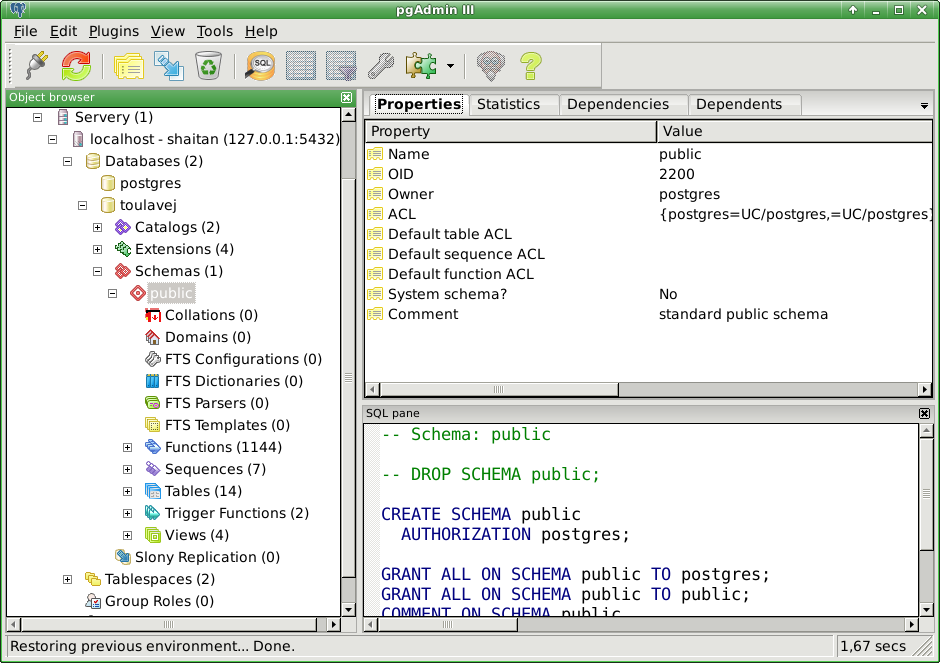
\includegraphics[width=8cm]{obrazky/pgadmin3.png}
				\caption{Desktopová aplikace pgAdmin III}
				\label{fig:pgadmin}
				(zdroj: snímek obrazovky)
			\end{center}
		\end{figure}
		\paragraph{Rozšíření}\label{par:rozsireni}Z existujících rozšíření mají spojitost s~vytvářeným projektem tři balíky. Prvním z~nich je PostGIS, který poskytuje podporu pro geografická data. Tento balík přidává do systému geometrii prvků a funkce pro práci s~nimi. Druhým rozšířením je pgRouting, který poskytuje funkce pro síťové analýzy. Posledním je rozšíření hstore. To usnadňuje práci s~daty uloženými v~datové struktuře \textit{pole(array)}. Všechny tři výše zmíněné projekty jsou šířeny pod licencí GNU \ac{GPL}.
		\begin{figure}[!h]
			\begin{center}
				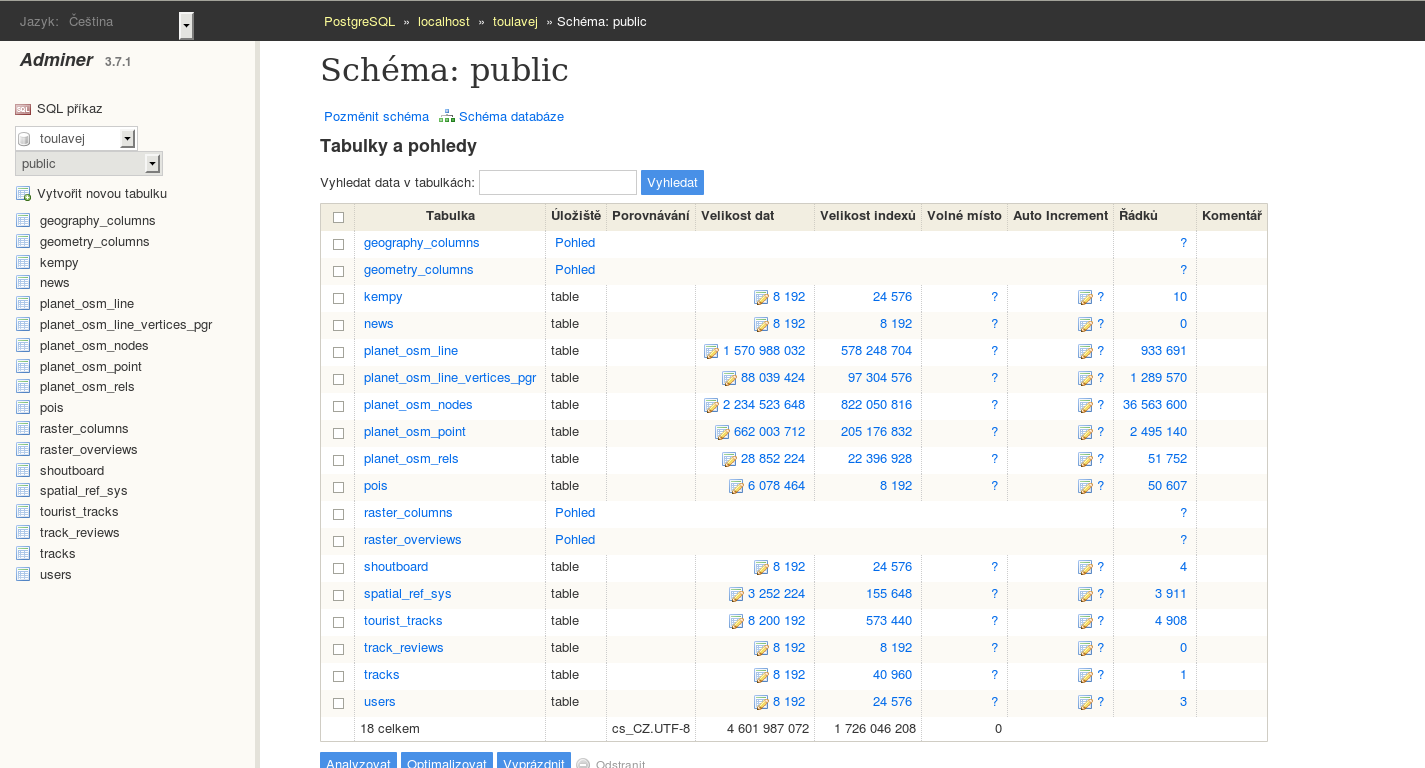
\includegraphics[width=10cm]{obrazky/adminer.png}
				\caption{Webová aplikace Adminer}
				\label{fig:adminer}
				(zdroj: snímek obrazovky)
			\end{center}
		\end{figure}			

                %%% ML: co je shell, neni vysvetleno, ctenar bez
                %%% hlubsi zkusenosti asi bude zmaten

                %%% -> ML: OK

		\paragraph{}Samotná databáze musí být nějak spravována. V~operačním systému Linux lze použít program psql, viz obr. \ref{fig:psql}, využívající příkazový řádek, grafické rozhraní pgAdmin III, viz obr. \ref{fig:pgadmin}, nebo \ac{PHP} program Adminer\footnote{\url{http://www.adminer.org/}}, viz obr. \ref{fig:adminer}. Každá z~uvedených variant má své výhody. Pro práci s~databází v~rámci skriptu napsaného pro shell\footnote{Textové uživatelské rozhraní v~Unixu a jemu podobných operačních systémech.} najde uplatnění právě příkazový řádek, pro práci na vzdáleném počítači lze využít Adminer, který se spouští přes webové rozhraní a pro práci na lokálním počítači se dá použít pgAdmin3.

%%%Programovací jazyky
	\section{PHP}
		\paragraph{} Pro zpracování dynamických požadavků na serveru je potřeba použít nějaký programovací jazyk. Tyto jazyky bývají označovány jako server--side. Patří mezi ně ASP, ASP.NET, C (při použití \ac{CGI} rozhraní), Java, Perl,\acs{PHP} a další. V~této aplikaci je použit poslední jmenovaný jazyk. \ac{PHP}\footnote{Název je rekurzivní zkratka.} je určený především pro tvorbu dynamických webových aplikací, ale lze ho využít i pro tvorbu konzolových a desktopových aplikací. PHP je platformně nezávislý programovací jazyk, který lze rozšířit mnoha knihovnami. Pro tvorbu webových aplikací se \ac{PHP} nejčastěji užívá se serverem Apache a databází MySQL. Tyto tři aplikace lze stáhnout v~jednom balíku, který je podle platformy označován zkratkou LAMP(pro Linux) nebo WAMP(pro Windows)\cite{wiki_php}.

                %%% ML: kde jsou pouzivany starsi verze, neni prilis jasne

                %%% -> ML: prepsal jsem to jako "řadě produkčích
                %%% serverů", ciste jsem dal do uvozovek

                %%% -> ML: posledni veta odstavce zni kostrbate, ale klidne ji nechte

		\paragraph{} Současná verze PHP je 5.5 (vydána ~20.6.2013\cite{php_net}), ale na řadě produkčích serverů jsou používány i starší verze jazyka. Při vývoji se užívá buď \uv{čisté} PHP a nebo v~podobě frameworků, které mají už naprogramované často užívané prvky. Tímto je usnadněna práce vývojáře, protože se může plně věnovat úkolu, který řeší. Frameworky také zajišťují větší bezpečnost, protože úkony jako přístup do databáze jsou již ošetřeny proti chybám a programátorovi stačí zavolat potřebnou funkci. Argumentem proti frameworkům je nižší rychlost zpracování požadavků a potřeba se naučit práci s~ním\cite{wiki_framework}. Pokud se framework používá na větších projektech, či počet projektů, kde je užit, je větší, tak čas, který práce s~frameworkem ušetří, je větší než doba, která je potřeba k~zvládnutí práce s~ním.
		\subsection{Framework Nette}
			\paragraph{} Jedná se o~open source framework českého původu, který je určený pro tvorbu aplikací v~PHP 5.  Autorem je David Grudl, ale v~současné době se o~vývoj stará organizace Nette Foundation. K~11.12.2013 byla uvolněna ke stažení verze 2.1.0 RC3, která je pod licencí NewBSD a GNU \ac{GPL}.  
			\paragraph{} Hlavním cílem je tvorba bezpečných aplikací. Mimo jiné je zde implementována ochrana před Cross-site scripting (XSS), která ošetřuje data z~uživatelských vstupů a zabraňuje tak, aby útočník podstrčil svůj vlastní kód. Ačkoliv je otázka bezpečnosti první v~seznamu výhod, není zdaleka poslední. Velmi silným argumentem pro jeho užití je snadné tvoření formulářů. Nette formuláře poskytují velké množství validačních pravidel. Automaticky generovaný validační javascriptový kód může být brán jako bonus.

                        %%% ML: Laděnka? vysvetlit
			\label{par:ladenka}
			\paragraph{} Při práci s~Nette je možné, ale ne nutné nastavit vývojový nebo produkční režim. Výhodou nastavení takovéhoto rozdělení je možnost nakopírování aplikace z~vývojového serveru na produkční a aplikace podle adresy serveru bere požadované parametry, např. jméno databáze, přihlašovací jméno a heslo a další. Ve vývojovém prostředí je dostupná knihovna Nette Diagnostics Debugger označovaná jako \uv{Laděnka}, viz obr. \ref{fig:ladenka}. Tato knihovna poskytuje množství nástrojů pro sledování aplikace. Její předností je přehledná vizualizace chyb, takže problémové pasáže není těžké najít a opravit.
		\begin{figure}[!h]
			\begin{center}
				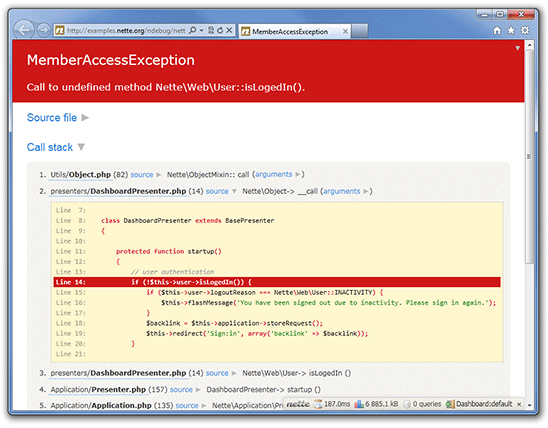
\includegraphics[width=10cm]{obrazky/ladenka.png}
				\caption{Grafické znázornění chyby pomocí \uv{Laděnky}}
				\label{fig:ladenka}
				(zdroj: Nette.org\cite{nette_web})
			\end{center}
		\end{figure}	

			\paragraph{} Velkou výhodou je, že v~českém prostředí má Nette aktivní komunitu uživatelů, kteří kromě tvorby mnoha komponent pořádají i pravidelné srazy uživatelů.  Uživatelé a vývojáři frameworku jsou též aktivní na fórech, kde lze řešit problémy v~aplikacích a chyby ve frameworku Nette.
			\subsubsection*{Návrhový vzor}
				\paragraph{} Návrhovým vzorem rozumíme architekturu aplikace. Jinými slovy se jedná o~určité části (vrstvy) aplikace, které zajišťují různé funkcionality. V~Nette se užívá architektura MVP (Model -- View -- Presenter).

                                %%% ML: zkuste odstavec prepsat (model)

                                %%% -> ML: OK

				\paragraph{Model} je vrstva, která se stará o~připojení k~databázi a která s~ní pracuje. Součástí modelu jsou funkce pro přístup k~databázi. Jedná se zejména o~výpis dat, jejich vkládání, změnu a mazání. Zbytek aplikace komunikuje s~model přes rozhraní, které model poskytuje. V~Nette obstarává funkce modelu knihovna Nette Database. Pro větší přehlednost se vytvářejí funkce, které vypisují potřebná data. Tím nedochází k~pokládání dotazů ve zdrojovém kódu Presenterů.

                                %%% ML: "V Nette se o tuto funkci
                                %%% starají šablony napsané latte."
                                %%% ???

                                %%% ML: chybi vysvetleni pojmu "sablona"

                                %%% -> ML: OK

				\paragraph{View} je vrstva, která vykresluje výsledek zadaného požadavku. V~Nette se o~tuto funkci starají šablony napsané v~latte. Šablonou rozumíme část zdrojového kódu webové stránky, který kontroluje vykreslení dat a vzhledu. Latte je šablonovací systém napsaný v~\ac{PHP}, ovšem díky němu je psaní šablon jednodušší, přehlednější a bezpečnější než kdybychom je psali v~čistém PHP.
				\paragraph{Presenter} je spojovací vrstva, která předává data z~modelu do view k~vykreslení a akce z~view zpracovává a předává modelu. Presenter je ekvivalentem Controlleru z~architektury MVC s~tím rozdílem, že Controller zpracovává i některé události uživatelského rozhraní.

	\section{JavaScript} %openLayers, Leaflet, jQuery a další
		\paragraph{} Každá webová stránka občas potřebuje zobrazit dynamický obsah, který bude okamžitě reagovat na uživatelské vstupy. V~aplikacích vytvořených v~programovacím jazyce Java zajišťuje jak práci na serveru, tak interakci na klientském počítači. Jazyk \ac{PHP} má ke zpracování uživatelských vstupů trochu jiný přístup. \ac{PHP} nedokáže dynamicky měnit obsah stránky bez nového načtení této stránky. Tento nedostatek jazyka se dá odstranit užitím jazyka JavaScript.

                %%% ML: zdroj?

                %%% -> ML: OK
		\begin{figure}[!h]
			\begin{center}
				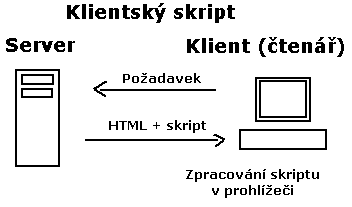
\includegraphics[width=5cm]{obrazky/klient_skript.png}
				\caption{Princip klientského skriptu, např. JavaScriptu}
				\label{fig:client}
				(zdroj: Jak psát web\cite{jakPsatWeb})
			\end{center}
		\end{figure}	
		\paragraph{} JavaScript byl vyvíjen jako jazyk Mocha ve firmě Netscape pro potřeby prohlížeče Navigator\cite{crockford}, ve kterém se objevil jako LiveScript. JavaScript je též znám jako ECMAScript. Díky svému jménu bývá často chybně spojován s~programovacím jazykem Java. Oba jazyky mají podobnou syntax, ale to mají i s~jinými jazyky, např. PHP nebo C++. Každý z~jazyků vytvořila jiná firma -- JavaScript byl vytvořen v~Netscapu a Java v~Sun Microsystems. JavaScript je hojně užíván pro tvorbu dynamického obsahu webových stránek, a proto se občas označuje za programovací jazyk webových stránek, ačkoliv se pro tvorbu internetových stránek používá jazyk \ac{HTML}.

                %%% ML: konec odstavce : "a ten pouze nahrát", čtenař
                %%% se
                %%% bude ptat, "nahrat kam", a proc "pouze", cela veta
                %%% by chtela
                %%% prepsat

                %%% -> ML: OK

		\paragraph{} Využití JavaScriptu je zejména v~tvorbě dynamických prvků na webových stránkách. Javascriptový kód je posílán ke klientovi na počítač, kde je zpracován, viz obr. \ref{fig:client}, interpreterem, který je součástí každého moderního prohlížeče. JavaScript je možné zapsat do \ac{HTML} souboru pomocí tagů \htmlTag{script}. Pokud se jedná o~delší skript, je lepší zapsat javascriptový kód do zvláštního souboru, pro který se standardně používá přípona js. Ve zdrojovém kódu stránky se zavolá pomocí \ac{HTML} tagu \htmlTag{script} s~tím, že se do vlastností přidá cesta k~souboru.
		\paragraph{AJAX} Asynchronní JavaScript A~XML je jedno z~běžných užití Java\-Scriptu, které umožňuje posílat \ac{XML} dotazy na server bez znovunačtení stránky. Server tento dotaz obslouží, vrátí výsledek a ten se zobrazí na stránce. Tato technika obnovování stránky si získala oblibu díky službám společnosti Google. Tento přístup je též užíván v~knihovnách jako jsou OpenLayers nebo Leaflet pro získání a zobrazení mapy.

		\begin{figure}[!h]
			\begin{center}
				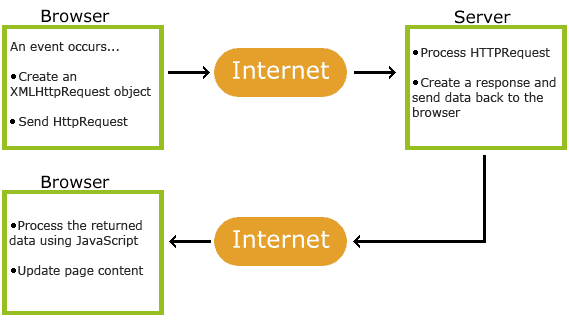
\includegraphics[width=5cm]{obrazky/ajax.png}
				\caption{Princip fungování AJAXu}
				\label{fig:ajax}
				(zdroj: W3 Schools\cite{w3school})
			\end{center}
		\end{figure}	

		\subsection{OpenLayers} %v2 v3
			\paragraph{} JavaScript lze využít pro tvorbu mnoha dynamických prvků stránek, ale pro složitější prvky je vhodnější použít nějaké existující nástroje. Pro tvorbu mapových aplikací existuje několik knihoven, které poskytují  API  pro usnad\-nění práce. Jednou z~takových knihoven je OpenLayers.
			\paragraph{} Jedná se o~knihovnu s~otevřeným kódem, která je šířena pod licencí BSD. OpenLayers byly vytvořeny firmou MetaCarta mezi roky 2005 a 2006 a od listopadu 2007 se o~jejich vývoj stará Open Source Geospatial Foundation\cite{wiki_ol}. Aktuální stabilní verze je 2.13.1, ale souběžně s~OpenLayers verzí 2 se vyvíjí i verze 3, která je dostupná ve verzi 3.0.0-beta1. OpenLayers~3 vzniká přepisováním původní verze a začleněním nových technologií, které umožňují využití HTML5 a CSS3\cite{ol}. Vytvoření mapy s~novou verzí je oproti minulé verzi rychlejší a výsledný kód je přehlednější.
			\paragraph{}OpenLayers jsou schopné zobrazit velké množství formátů -- od rastrových dat ve formátu JPEG nebo PNG až po vektorová data GeoJSON či GML. Data lze připojit přímo z~disku nebo je lze získat pomocí WMS nebo WFS služby. Velkým plus této knihovny je velice dobře zpracovaná dokumentace a vzorové příklady, které pomohou při tvorbě mapové aplikace. 
		\subsection{Leaflet}
			\paragraph{} Druhou knihovnou, kterou lze užít na tvorbu webové mapové aplikace, je javascriptová knihovna Leaflet. Jedná se o~moderní knihovnu srovnatelnou s~OpenLayers 3. Leaflet se dá též použít pro zobrazení aplikace na mobilních zařízeních. Stejně jako OpenLayers 3 je i Leaflet stále ve vývoji (od listopadu 2013 je dostupná verze 0.7.1)\cite{Leaflet}, takže některé prvky stále nejsou plně funkční či chybí úplně. Dobře zdokumentované API a návody pro začátečníky jsou velice dobrým pomocníkem při tvorbě map, stejně tak i různé zásuvné moduly, které vytvořili členové komunity.
		\paragraph{} Ačkoliv Leaflet a OpenLayers 3 jsou modernější, pro vývoj aplikace byla použita stávající verze OpenLayers v2. Původně zvažovaný Leaflet byl zamít\-nut kvůli problémům s~připojením vektorových vrstev a kvůli tomu, že se stále jedná o~vývojovou verzi. Ze stejného důvodu nebyla použita ani knihovna OpenLayers 3.

                %%% ML: najdete mene zavadejici nazev pro tuto
                %%% kapitolu...

                %%% -> ML: OK

	\section{Vzhled aplikace}

        %%% ML: "grafika uzivatelskeho rozhrani" slysim poprve, zkuste
        %%% spise operovat s pojmem "design" nebo navrh UI

        %%% ML: "tvorba grafiky" ??? design ...

        %%% -> ML: OK

		\paragraph{} Důležitým prvkem webové stránky je její grafické provedení, protože špatně vytvořený vzhled webu může odradit potenciální zákazníky. Důležitost návrhu \ac{UI} dokazuje i to, že dost firem vyvíjejících webové stránky a~aplikace má ve svém týmu člověka, který se věnuje zejména tvorbě grafických návrhů aplikací.

                %%% ML: prvku ceho?

		\paragraph{} Hlavním nástrojem pro určení pozice, barvy, velikosti a chování prvků aplikace při zmenšení/zvětšení okna jsou \ac{CSS}. Vzhled stránky může být definován v~sekci \htmlTag{head} souboru s~HTML kódem stránky nebo pomocí vlastnosti \textit{style} přímo u~prvku, ale častěji se kvůli přehlednosti využívá zapsání do samostatného souboru, který se do HTML dokumentu importuje podobně jako javascriptový soubor. Kaskádovými styly lze modifikovat vzhled všech HTML prvků. 

                %%% ML: "zapsani" ??

                %%% ML: "První možností je užítí na všechny prvky
                %%% stejného typu" - zkuste prepsat...

		\paragraph{} Kaskádové styly mohou ovlivňovat vzhled prvků na třech úrovních.
				\begin{itemize}
					\item Na úrovni \ac{HTML} tagů lze nastavit jednotný vzhled pro všechny tagy stejného typu, např. stejný vzhled všech nadpisů v~tagu \htmlTag{h1}.
					\item Pro jednotlivé třídy, které se volají v~\ac{HTML} tagu, lze nastavit styl pomocí vlastnosti \textit{class}.
					\item Unikátním prvkům může být nastaven styl podobně jako v~případě tříd s~tím rozdílem, že se jméno stylu zapisuje do vlastnosti \textit{id}.
				\end{itemize}

                %%% ML: "vrstvit" nezni moc pekne ...

                                %%% -> ML: OK

		\paragraph{} Aby bylo možno dosáhnout požadovaného výsledku, umožňují kaskádové styly kombinovat jednotlivá pravidla, jak je zobrazeno na příkladu webu Seznam.cz (viz obr. \ref{fig:seznam}). Ne všechny prohlížeče zobrazují všechny stránky stejně. U~Microsoft Internet Exploreru je interpretace CSS stylů odlišná od jiných prohlížečů, což vede vývojáře k~vytváření speciálních pravidel pro tento prohlížeč.
		\begin{figure}[!h]
			\begin{center}
				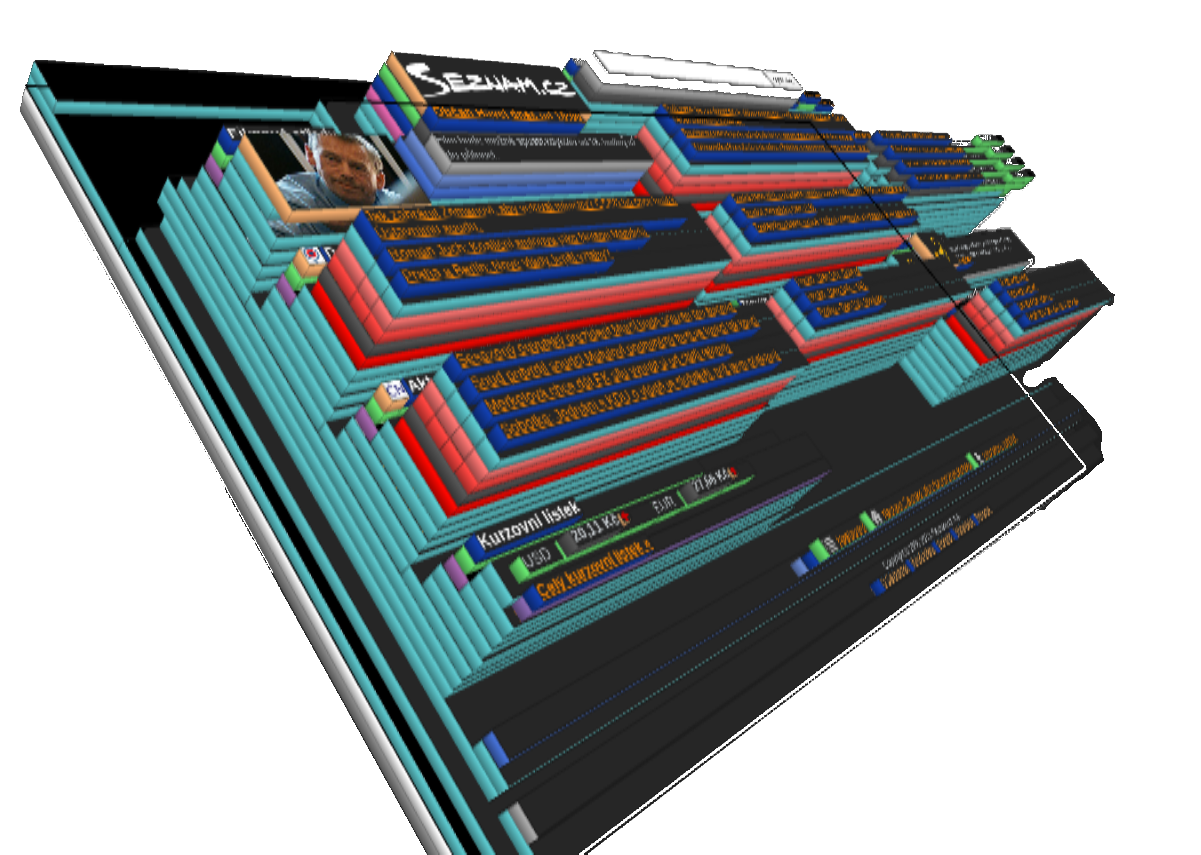
\includegraphics[width=12cm]{obrazky/css_vrstvy.png}
				\caption{Zobrazení CSS vrstev webu Seznam.cz}
				\label{fig:seznam}
				(zdroj: Seznam.cz)
			\end{center}
		\end{figure}	

                %%% ML: odkaz na Twitter, poznamka pod carou, vysvetleni...

		\paragraph{} Pro usnadnění práce vývojářů vznikly různé šablony a frameworky. V~pří\-padě vyvíjené aplikace byl použit Bootstrap (v2.2.2) -- framework s~otevřeným zdrojovým kódem vytvořený pro Twitter\footnote{\url{https://twitter.com/}} v~polovině roku 2010. Ve verzi 2 byla přidána podpora responsivního designu, což zaručuje správné zobrazení aplikace i na mobilních zařízeních\footnote{Aplikace pozná, na jak velkém displeji je zobrazena, a podle toho vybere odpovídající design pro optimální zobrazení obsahu.}. Začátkem prosince 2013 byl vydán Bootstrap ve verzi 3.0.3, která má v~základu nastavený responzivní design a bere ohled na mobilní zařízení.
%%%%%%%%%%%%%%%%%%%%%%%
%%%%% 	VÝVOJ APLIKACE	   %%%%%
%%%%						      %%%%
%%%							  %%%
%%								     %%
%									 %
\chapter{Vývoj aplikace}
		\section{Databáze}
Databáze je důležitým prvkem aplikace \uv{Toulavej} -- jsou zde uloženi registrovaní uživatelé, příspěvky v~diskuzi a další data včetně dat \ac{OSM}.
			\subsection{Datový model}
				\paragraph{}  Databáze byla vytvářena postupně podle toho, které tabulky byly potřeba. Všechny tabulky a sloupce jsou pojmenovány anglicky. V~obrázku \ref{fig:db} jsou vidět tabulky a vztahy mezi nimi. V~schématu nejsou zobrazeny tabulky vzniklé importem dat planet\_osm a tabulky rozšíření PostGIS. 
				\paragraph{}Tabulka \textit{news} je určena pro ukládání událostí, které jsou zveřejňovány jako novinky. Zde se evidují pouze položky \textbf{id} jako primární klíč, \textbf{user\_id} jako cizí klíč na tabulku \textit{users}, \textbf{note} s~novinkou a čas vytvoření (\textbf{created}).

				%%%ChV: Tento odstavec  přibyl
				\paragraph{}Pro ukládání informací o~obrázcích slouží tabulka \textit{images}. Primárním klíčem je sloupec \textbf{id}. Tabulka dále obsahuje cizí klíč \textbf{user\_id} odkazující na tabulku \textit{users}. Ten určuje, kdo daný obrázek nahrál. Pojmenování obrázku je v~sloupci \textbf{name}. Dalšími sloupci jsou čas vytvoření(\textbf{created}), poznámka(\textbf{note}) a jméno odpovídajícího souboru(\textbf{filename}).

                                %%% ML: "Zde je velice častý výskyt
                                %%% hodnoty NULL." proc neni
                                %%% vysvetleno...

                                %%% ML: co je hstore, proc bylo
                                %%% pouzito, chybi vysvetleni nebo
                                %%% odkaz na text, kde to bude
                                %%% vysvetleno...

				\paragraph{}Další v~pořadí je tabulka \textit{pois} odvozená od bodové vrstvy dat \ac{OSM}. Vznikla vybráním bodů, které by mohly být pro uživatele nějakým způsobem zajímavé. Hlavní sloupce jsou \textbf{osm\_id} pro primární klíč a \textbf{way} pro geometrii. Sloupce \textbf{amenity, historic, leisure, man\_made, name, natural, religion, shop a tourism} obsahují informaci o~typu prvku. Zde je velice častý výskyt hodnoty NULL, protože řada vlastností vylučuje existenci jiné hodnoty u~dalších atributů. Sloupec \textbf{tags} užívá rozšíření hstore, viz kap. \ref{par:rozsireni}, a jsou v~něm uvedeny další informace.
		\begin{figure}[!h]
			\begin{center}
				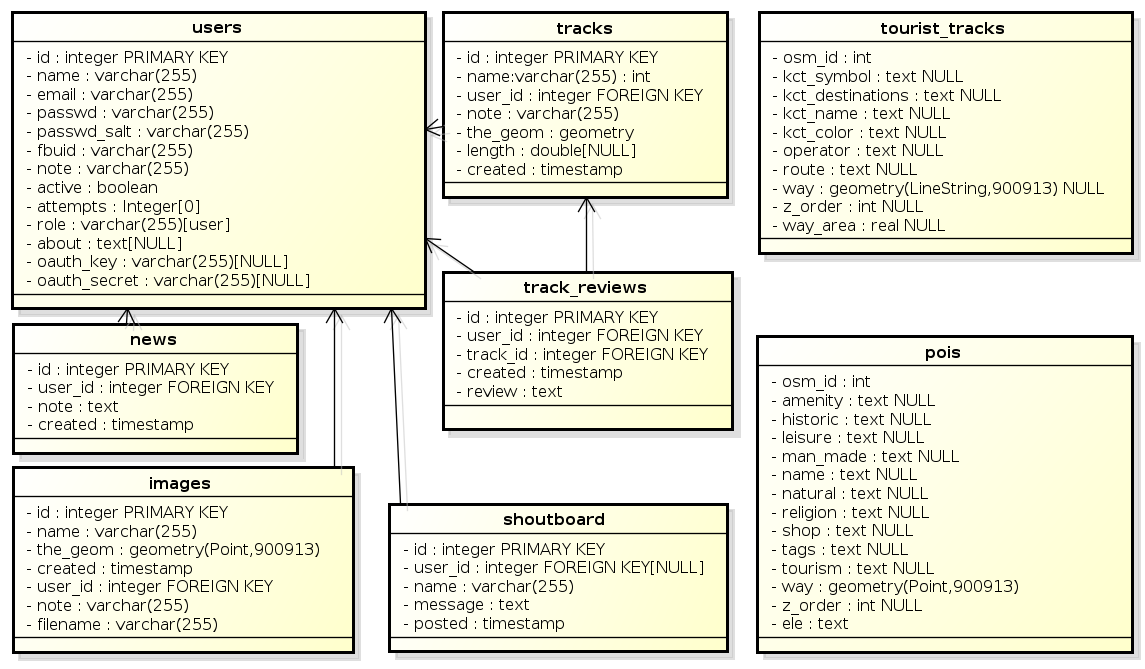
\includegraphics[width=13cm]{obrazky/datovy_model.png}
				\caption{Datový model databáze projektu Toulavej}
				\label{fig:db}
			\end{center}
		\end{figure}
                        \paragraph{} Další tabulkou odvozenou z~liniové vrstvy dat \ac{OSM} jsou \textit{tourist\_tracks}. Stejně jako \textit{pois} nese sloupec s~primárním klíčem označení \textbf{osm\_id}. Sloupec \textbf{kct\_color} určuje barvu turistické stezky bez ohledu na druh značky. Ten je zohledněn v~\textbf{kct\_symbol}. Možné cíle trasy(pokud jsou uvedeny) udává \textbf{kct\_destinations}. Pokud má trasa nějaké jméno, je uvedeno v~\textbf{kct\_name}. Zřizovatel trasy je uveden v~\textbf{operator}. V~poli \textbf{route} je uveden typ cesty. Geometrii lze nalézt ve sloupci \textbf{way}. Atribut \textbf{way\_area} určuje plochu ohraničenou uzavřeným liniovým prvkem.

                        %%% "a délka je v \textbf{length}" delka ceho,
                        %%% nutno vysvetlit, a proc se uklada
                        %%% explicitne... ?

			\paragraph{} Tabulka \textit{tracks} slouží k~ukládání uživateli vloženými trasami. Na uživatele, který příspěvek vložil, odkazuje atribut \textbf{user\_id}. Geometrii lze najít v~sloupečku \textbf{the\_geom} a délka trasy je uložena v~\textbf{length}. Délka se ukládá explicitně, aby pro výpis v~\textit{Seznamu tras} nebo \textit{Detailu trasy} nebylo nutné vytvářet novou funkci a bylo možné použít dostupné řešení.  Do pole \textbf{note} se vkládají poznámky či možné cíle trasy. \textbf{Id} určuje primární klíč a \textbf{created} je čas uložení do databáze. Na tuto tabulku se váže přes cizí klíč \textbf{track\_id} tabulka \textit{track\_reviews}, která slouží k~ukládání komentářů a hodnocení k~cestám. \textit{Track\_reviews} se váží přes \textbf{user\_id} na tabulku \textit{users}. Dále je zde samotný text (\textbf{review}) a časová známka, kdy byl příspěvek vložen (\textbf{created}).
			\paragraph{}\label{par:users}Tabulka \textit{users} slouží k~ukládání dat o~registrovaných uživatelích. Pole \textbf{id} je primární klíč, které má výchozí hodnotu nastavenou na další číslo v~pořadí. Pole \textbf{name} je jméno, které zadává uživatel při registraci nebo které se vezme z~profilu na Facebooku. Toto jméno lze v~nastavení změnit. Tabulka obsahuje pole s~emailem, který spolu s~heslem slouží k~přihlášení do aplikace. Pokud je uživatel připojen přes Facebook, uloží se jeho identifikace na Facebooku do pole \textbf{fbuid}. Pole \textbf{active} slouží k~případnému znemožnění přihlášení uživatele a pole \textbf{attempts} ukazuje počet neúspěšných pokusů o~přihlášení. Pokud dosáhne jejich počet určitého množství, tak se účet zablokuje. Sloupec \textbf{role} udává, jaká práva má daný uživatel. V~systému jsou tři typy rolí (guest, user a admin) ale pouze user a admin se ukládají do tabulky. Volitelné pole \textbf{about} umožňuje uživateli napsat o~sobě pár informací a \textbf{note} slouží k~zapsání poznámky pro administrátora. Sloupce \textbf{oauth\_key} a \textbf{oauth\_secret} jsou určeny pro přihlašování do \acl{OSM}.

                        %%% ML: tomuto odstavci nerozumim...
			%%%ChV: odstavec měl být někde jinde

			\subsection{Naplnění databáze}
				\paragraph{} Před zahájením samotného naplnění databáze bylo potřeba aktivovat rozšíření. Jednalo se o~\textit{PostGIS} rozšíření pro práci s~geografickými daty, \textit{PgRouting} pro plánované vyhledávání cest mezi zadanými body a \textit{hstore} pro usnadnění práce s~daty ve sloupcích \textbf{tags}. Na tyto úkony je potřeba administrátorský přístup, takže potřebné modifikace v~databázi na serveru \textit{geo102} provedl Ing. Landa.
				\paragraph{} V~momentě, kdy byla databáze připravena, bylo možné vytvořit tabulky a nahrát data. Pro získání dat OpenStreetMap byla použita internetová stránka \url{http://download.geofabrik.de/europe/czech-republic.html}, kde jsou data Planet.osm rozdělena podle kontinentů a zemí. Tato data jsou každý den aktualizována. Nejjednodušším způsobem, jak nahrát data do databáze, je pomocí konzolové aplikace \textit{osm2pgsql}. Při importu dat může dojít k~tomu, že užívaný počítač nemá potřebnou operační paměť. Program \textit{osm2pgsql} tento problém řeší pomocí tzv. \textit{slim modu}, ve kterém jsou využita dočasná úložiště. Ta zmenší velikost potřebné operační paměti. Databáze České republiky zabírá zhruba 4 GB paměti, ovšem ne všechna data jsou pro projekt potřebná. V~případě turistických stezek byla potřebná data uložena do speciální tabulky, protože jejich výběr z~původní tabulky za pomoci SELECTu nebo VIEW byl zdlouhavý. Ze stejného důvodu byly vybrány i zájmové body. Při prvním nahrání databáze vznikl problém se získáním údajů z~pole \textbf{tags}. V~dokumentaci \textit{PostgreSQL} na stránkách aplikace byl uveden příklad, jak je získat. Tento problém poté odpadl s~aktivací rozšíření \textit{hstore}. Kvůli výsledné velikosti databáze je zvažováno, že po zprovoznění vyhledávání cest budou tabulky s~nepotřebnými daty odstraněny. Aby se k~datům dalo přistupovat z~webové aplikace, bylo potřeba správně nastavit přístupová práva.
				\paragraph{} V~neposlední řadě bylo potřeba doplnit tabulky, které nevznikají z~dat \acl{OSM}:
					\begin{itemize}
						\item news -- novinky generované při některých akcích či zadané administrátorem
						\item images -- fotografie vložené uživateli
						\item shoutboard -- tabulka pro diskuzi
						\item track\_reviews -- komentáře a články k~trase
						\item tracks -- uživateli zadané trasy
						\item users -- informace o~uživatelích včetně jejich přihlašovacích údajů
					\end{itemize}
Většina těchto tabulek neobsahuje geografická data, jenom tabulky \textit{tracks} a \textit{images} mají geometrickou složku popisu geodat. Tyto tabulky jsou po vytvoření prázdné. Jen do tabulky \textit{users} byly vloženy administrátorovy přihlašovací údaje.
			\subsection{Aktualizace databáze}
				\paragraph{} Protože se data \acl{OSM} neustále vyvíjejí a zpřesňují, je potřeba je jednou za čas aktualizovat. Vzhledem k~tomu, že se jedná o~časově náročnou činnost (import dat OpenStreetMap trvá na serveru kolem 1 hodiny), byl vytvořen skript, který provede potřebné kroky automaticky poté, co je předchozí úkol hotov. Skript postupuje v~následujících krocích.
		\begin{enumerate}
			\item Stáhne aktuální data pomocí příkazu \textit{wget}  z~\url{http://download.geofabrik.de/europe/czech-republic-latest.osm.bz2}.
			\item Rozbalí data pomocí programu \textit{bunzip2}.
			\item Za užití \textit{osm2pgsql} s~parametry \textit{ -\--slim  -\--cache--strategy dense -\--hstore --d vorlichr\_dp} importuje data do databáze.
			\item Program psql vytvoří tabulku \textit{tourist\_tracks} podle SELECTu ze souboru \textit{hiking\_routes.sql}.
			\item Ze souboru \textit{pois.sql} použije \textit{psql} dotaz na vytvoření tabulky \textit{pois}.
			\item Spustí se skript, který správně nastaví přístupová práva k~databázi.
			\item V~posledním kroku skript smaže stažený soubor.
		\end{enumerate}
			\paragraph{} V~momentě, kdy bude plně funkční vyhledávání tras pomocí pgRoutingu, do programu přibudou další kroky, které provedou potřebné úpravy. Jedná se o~vytvoření tabulky se silnicemi a cestami, vypočítání geometrie sítě a nastavení parametrů potřebných pro vyhledávání.

		\begin{figure}[!h]
			\begin{center}
				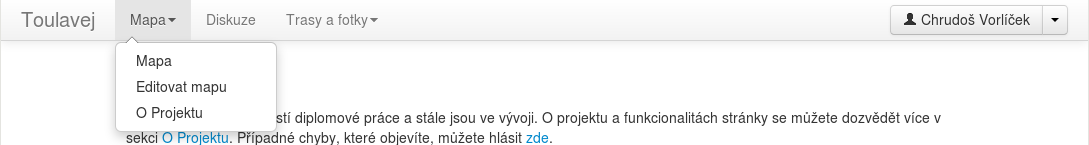
\includegraphics[width=12cm]{obrazky/toulavej/menu_puv.png}
				\caption{Původní menu}
				\label{fig:menu_puv}
			\end{center}
		\end{figure}	

		\section{Vzhled a styly}

                %%% ML: reference na obrazky je vhodne komentovat,
                %%% napr. (viz obr.~\ref{fig:menu_puv})

			\paragraph{} Při tvorbě vzhledu byla snaha vytvořit jednoduché rozhraní. Z~hlediska lepšího využití prostoru bylo menu navrhnuto jako lišta. Původní navigační panel, viz obr.~\ref{fig:menu_puv}, obsahoval dvě rozbalovací menu, ale po konzultaci s~Ing. Landou bylo shledáno toto rozvržení nevhodným. Jednalo se např. o~zařazení stránky \textit{O~Projektu} pod záložku \textit{Mapa}. Předělané menu, viz obr.~\ref{fig:menu_nove}, je přehlednější.
		\begin{figure}[!h]
			\begin{center}
				
\includegraphics[width=12cm]{obrazky/toulavej/menu_nove.png}
				\caption{Nové menu}
				\label{fig:menu_nove}
				(zdroj: snímek obrazovky)
			\end{center}
		\end{figure}	
			\paragraph{} Ve frameworku Bootstrap jsou vytvořeny styly pro většinu běžných prvků -- navigační lišta je jedním z~nich. Díky tomu je snadné poskládat prvky do požadovaného vzhledu. Ačkoliv byl použit Bootstrap, tak pro některé prvky bylo potřeba vytvořit nové styly či upravit stávající, protože existující nevyhovovaly. Jedním z~příkladů je odsazení textů. V~původní verzi Bootstrapu začínal text přímo na kraji stránky, což není pro uživatele příliš příjemné. Nové styly byly většinou tvořeny pro unikátní prvky jako je např. mapové pole.
		\begin{figure}[!h]
			\begin{center}
				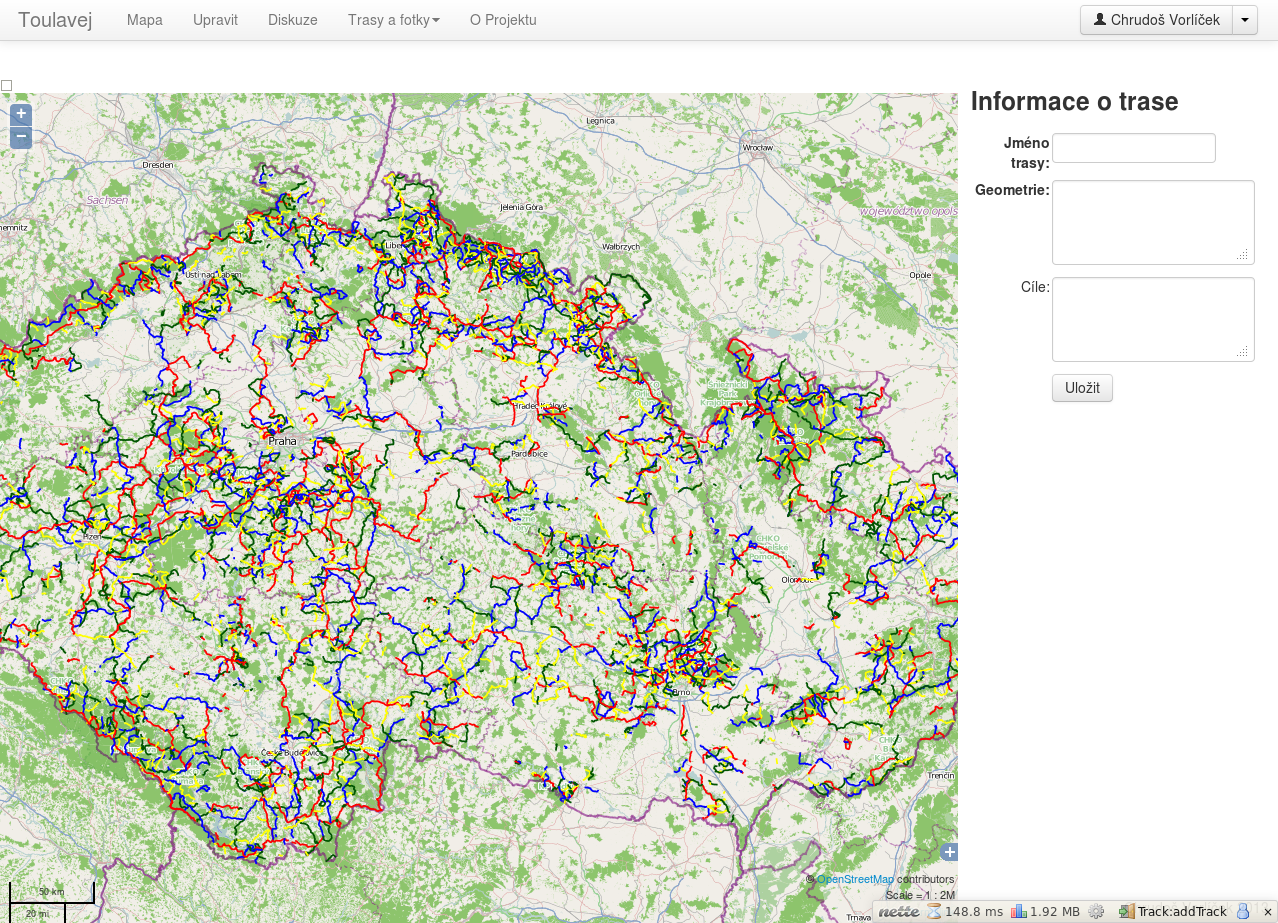
\includegraphics[width=9cm]{obrazky/toulavej/addTrack.png}
				\caption{Styl mapového pole pro přidávání tras}
				\label{fig:addTrack}
				(zdroj: snímek obrazovky)
			\end{center}
		\end{figure}	
			\paragraph{} Mapových oken je v~aplikaci víc a mají různá nastavení stylů. První je v~samotné sekci \textit{Mapa} a hlavním rysem tohoto prvku je malé odsazení od spodního a bočních krajů. Stejný rys má i druhé okno, které se nachází v~sekci \textit{Upravit}. To je ale navíc rozděleno na mapovou a textovou část. Poslední styl mapy je společný pro tři mapová okna. Jedná se o~přidání vlastní trasy, zobrazení trasy na mapě a přidání fotografie k~souřadnicím. Tento styl se vyznačuje odsazením od pravého kraje, takže zde vznikne místo pro Informace o~trase -- buď vypsané v~tabulce nebo vstupní formulář pro ně, viz obr.~\ref{fig:addTrack}.
			\paragraph{}\label{par:grafikaId} Z~grafického hlediska bylo největším problémem propojení aplikace Toulavej s~editorem iD, protože tato aplikace má své vlastní styly. Některé třídy stylů měly stejné názvy a  styly editoru tak přepisovaly pravidla aplikace. Tento problém byl vyřešen přepsáním pravidel, která se vzájemně rušila, tak, aby byla stejná. Ačkoliv většina aplikace byla přepsána úspěšně, v~některých místech stále není úprava provedena, např. v~editoru iD chybí tlačítku lokalizovat popis po najetí myši, viz obr.~\ref{fig:error_locate}.
		\begin{figure}[!h]
			\begin{center}
				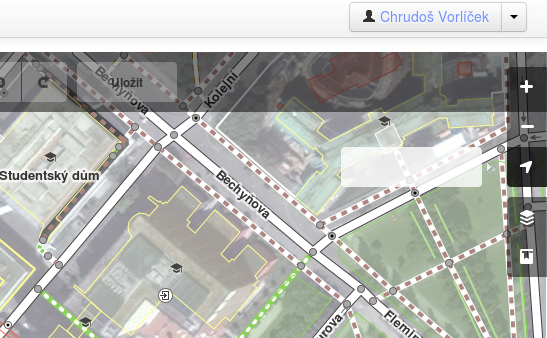
\includegraphics[width=7cm]{obrazky/toulavej/chyba_locate.png}
				\caption{Chyba stylů}
				\label{fig:error_locate}
			\end{center}
		\end{figure}	


                %%% ML: nazev kapitoly neni jasny, hned v prvni vete
                %%% mluvite o "mapovych oknech"... 

		%%% ChV: lepší název mě nenapadl, pokud mě něco napadne, změním to
		%%% ChV: trochu jsem přepracoval následující text

		\section{Turistická mapa}
			\paragraph{} Mapová okna mají nejen své vlastní styly, ale i své vlastní konfigurace, které bylo třeba vytvořit. Hlavní částí aplikace je mapa, která zobrazuje turistické stezky, zájmové body a fotografie. Mapy, které slouží k~vkládání fotografií a tras, jsou odvozeny od této mapy. Stejně tak i mapa pro zobrazení tras vložených uživateli. Jejich konfigurace vznikla odvozením od konfigurace hlavní mapy s~tím rozdílem, že je k~nim připojena rastrová vrstva turistických stezek.
			\paragraph{} Pro okno editoru iD nemusela být vytvářena žádná speciální konfigurace mapy, protože celá aplikace už je vytvořena.  Problémy spočívaly v~dříve popsaném nastavení \ac{CSS} stylů, viz kap. \ref{par:grafikaId}, a v~nastavení autorizace přes oAuth.%, viz kap. \ref{par:oAuthId}.

			\paragraph{} Do hlavní mapy bylo kromě podkladové mapy potřeba připojit i další vrstvy. První v~pořadí byla připojena přes službu \ac{WFS} data turistických stezek. Pro získání informací o~prvku byla vytvořena funkce, která je vypíše (pokud jsou k~dispozici) a zvýrazní vybranou stezku, viz obr.~\ref{fig:infoTrack}. Informace, které mohou být zobrazeny, jsou jméno a cíle stezky, celková délka a barva trasy.

                        %%% Nikde neni vysvetlen rozdil mezi WFS a
                        %%% WMS, alespon o tom nevim, to je potreba
                        %%% nekde doplnit nebo pridat odkaz na
                        %%% kapitolu, kde je to vysvetlo, ctenar se
                        %%% bude ptat "proc je nacitani WFS tak
                        %%% zdlouhave", to je potreba vystetlit

			\paragraph{}Protože služba \ac{WFS} přenáší vektorová data, načítání vrstvy turistických tras \ac{kct} bylo zdlouhavé. Z~toho důvodu byla vrstva turistických tras připojena ještě službou \ac{WMS}, která data poskytuje jako rastry, jejichž načítání je rychlejší. To je způsobeno tím, že \ac{WMS} přenáší obrazovou reprezentaci dat, zatímco \ac{WFS} přenáší samotná data. Mapa je nastavena tak, že do měřítka 1 : 250 000 zobrazuje rastry s~turistickými trasami  a při měřítkách větších než 1 : 250 000 jsou k~dispozici data vektorová.
		\begin{figure}[!h]
			\begin{center}
				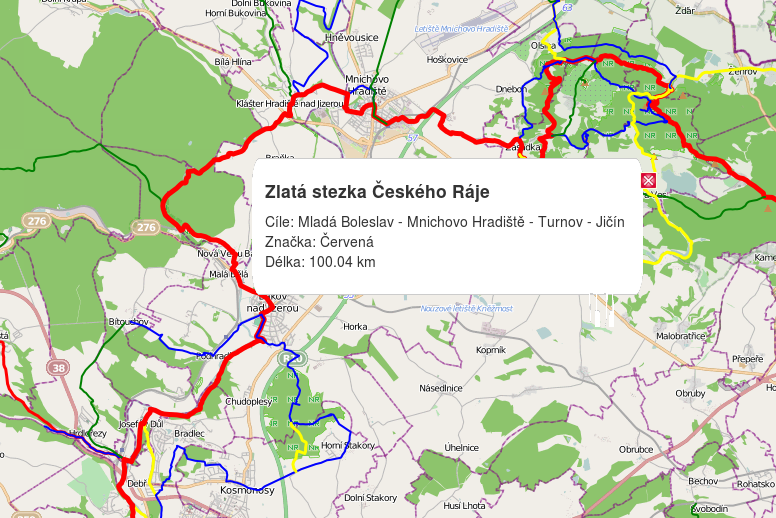
\includegraphics[width=9.4cm]{obrazky/toulavej/infoTrack.png}
				\caption{Informace o~turistické trase}
				\label{fig:infoTrack}
				(zdroj: snímek obrazovky)
			\end{center}
		\end{figure}	

			\paragraph{} Abychom vůbec mohli použít \ac{WMS} a \ac{WFS} vrstvy z~dat, která jsou uložena v~databázi, musí být nastaven Geoserver, vrstvy musí být publikovány a pro \ac{WFS} službu musí být na serveru přítomen soubor, který zpracovává proxy dotazy. Toto je dáno tím, že se z~OpenLayers nelze připojit ke Geoserveru a komunikovat s~ním přímo. 

				%%%ChV: přibyly odstavece
			\paragraph{} Služba \ac{WFS} byla použita i k~připojení vrstev se zájmovými body. Ty jsou rozděleny do několika kategorií:
					\begin{itemize}
						\item fotogalerie -- zobrazuje fotografie na místě, odkud pocházejí
						\item hrady, zříceniny
						\item informace -- kromě stánků s~informacemi zobrazují tyto prvky i směrové cedule a informační tabule a mapy
						\item náboženské objekty -- jedná se jak o~kostely, chrámy a synagogy, tak i různé kříže a křížové cesty
						\item občerstvení -- hospody, stánky, restaurace aj.
						\item prameny
						\item stromy
						\item vrcholy
					\end{itemize}	
Jednotlivé vrstvy vznikly jako VIEW\footnote{VIEW je struktura, ve které je uložen SQL dotaz. Slouží k~ukládání často volaných nebo složitých dotazů} z~tabulky \textit{pois}. Tímto bylo možno pro každý typ zájmového bodu získat ze sloupce \textbf{tags} potřebné informace.

			\paragraph{} Pro odlišení jednotlivých vrstev a prvků podle jejich atributů byla vytvořena pravidla, podle kterých se prvku přiřazuje příslušný symbol. Pro vrstvu turistických tras existují pravidla, která jednotlivým trasám přiřadí jednu ze čtyř barev: červenou,modrou,zelenou a žlutou. Pro bodové prvky byly vytvořeny symboly, viz obr. \ref{fig:symboly}.
			
		\begin{figure}[!h]
			\begin{center}
				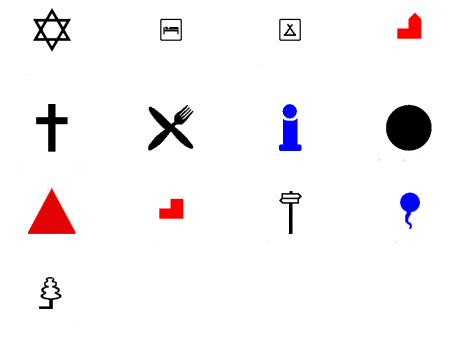
\includegraphics[width=6cm]{obrazky/toulavej/symbols.png}
				\caption{Symboly použité pro zobrazení bodových vrstev}
				\label{fig:symboly}
			\end{center}
		\end{figure}	

			\paragraph{}Vzhledem k~množství prvků, které jsou takto zobrazeny, bylo nastaveno měřítko, od kterého se data zobrazují, na větší nebo rovno 1 : 54 000. Toto měřítko odpovídá na stupnici, kterou užívají OpenLayers jako výchozí, hodnotě přiblížení 13. Pro tyto vrstvy nelze pro malá měřítka použít \ac{WMS} verzi, protože to činí mapu nepřehlednou a v~některých místech vrstva úplně překryje podkladovou mapu, viz obr. \ref{fig:food}.
		
		\paragraph{}Pro zobrazení informací o~jednotlivých prvcích byly vytvořeny funkce podobné té, která vypisuje informace o~turistických trasách.

\begin{figure}[!h]
			\begin{center}
				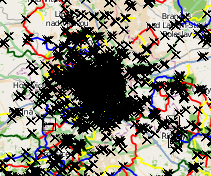
\includegraphics[width=6.7cm]{obrazky/toulavej/food.png}
				\caption{Překrytí podkladové mapy vrstvou  \textit{Občerstvení} na území Prahy}
				\label{fig:food}
				(zdroj: snímek obrazovky)
			\end{center}
		\end{figure}	

		%%%ChV: zde končí nová část

			\paragraph{} V~neposlední řadě byly do mapy přidány ovládací prvky jako zoom, permanentní odkaz, měřítko a přehledka. Pokud je uživatel přihlášený, tak může pomocí funkce \textit{Upravit} přejít do editačního módu na souřadnicích, kde momentálně leží střed mapy. Pokud má uživatel účet na Facebooku a má ho propojený s~aplikací, může sdílet mapu s~přáteli. Tlačítka \textit{Přidat trasu} a \textit{Přidat fotku} přesměrují uživatele na mapu s~formulářem pro přidání nové trasy, resp. fotografie.
			
		\section{Uživatelské rozhraní}
			\subsection{Přihlašování uživatelů}

                        %%% ML: zde by mel byt odkaz na kapitolu, kde
                        %%% se mluvi o datovem modelu DB (low priority)

				\paragraph{}K ukládání registrovaných uživatelů byla v~databázi vytvořena tabulka \textit{users},viz kap. \ref{par:users}). Tabulka ukládá data jak uživatelů registrovaných na stránkách, tak uživatelů přihlášených přes Facebook.
                                %%% ML: "je potřeba se registrovat na
                                %%% stránce" zkuste napsat jasneji
					\paragraph{} Pokud uživatel chce využívat všechny služby, které aplikace poskytuje, musí mít na webu vytvořený svůj účet. Ten lze vytvořit dvěma způsoby.
					\subsubsection{Bez Facebooku} 
						\paragraph{}Pokud uživatel nemá účet na sociální síti Facebook nebo z~nějakého důvodu tento účet použít nechce, je na webu vytvořen formulář, který slouží k~registraci nových uživatelů, viz obr.  \ref{fig:regForm}.
		\begin{figure}[!h]
			\begin{center}
				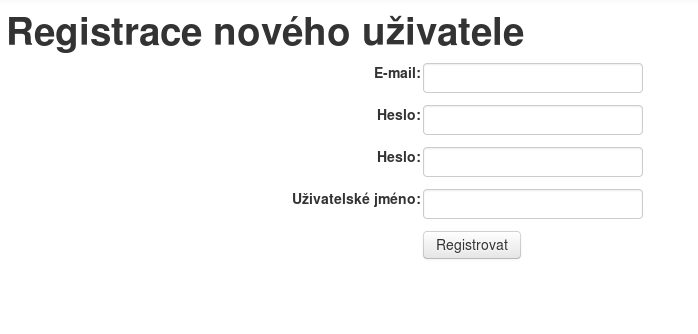
\includegraphics[width=8cm]{obrazky/toulavej/regForm.png}
				\caption{Registrační formulář aplikace \uv{Toulavej}}
				\label{fig:regForm}
				(zdroj: snímek obrazovky)
			\end{center}
		\end{figure}	
 Formulář je opatřen i pasivním filtrem proti robotům, kteří by opakovaně vytvářeli účty a zahlcovali tak databázi. Navíc by tím získali přístup k~přidávání tras a fotek, což je nežádoucí. Teoreticky by mohlo dojít k~ukládání s~webem nesouvisejících fotografií. Přístup k~editaci dat \ac{OSM} by tímto nezískali, protože by museli mít zřízený účet na \acl{OSM}. 

					\paragraph{}Po registraci je uživatel okamžitě přihlášen a přesměrován na domovskou stránku. Uživatel s~již zřízeným účtem se přihlásí pomocí přihlašovacího formuláře, viz obr. \ref{fig:login}. Pomocí volby \textit{Pamatuj si mě} může uživatel zvolit, že chce zůstat přihlášen i po opuštění stránky.
		\begin{figure}[!h]
			\begin{center}
				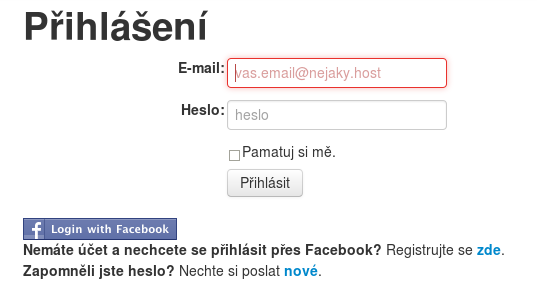
\includegraphics[width=7cm]{obrazky/toulavej/login.png}
				\caption[Přihlašovací formulář s~odkazem na přihlášení na Facebook]{Přihlašovací formulář s~odkazem na přihlášení na \ac{Fb}, registraci a obnovu zapomenutého hesla}
				\label{fig:login}
				(zdroj: snímek obrazovky)
			\end{center}
		\end{figure}	

				\subsubsection{S~Facebookem} 
                                %%% ML: TODO
					\paragraph{}Pro přihlášení přes \ac{Fb} je v~sekci \textit{Přihlásit} odkaz na přihlášení, viz obr. \ref{fig:login}. Ten přesměruje uživatele na stránky \acl{Fb}u, kde se uživatel přihlásí. Pokud je již na \ac{Fb} přihlášen, tento krok je vynechán. Dalším krokem při prvním přihlášení je udělení oprávnění pro přístup k~informacím a ke sdílení dat. V~momentě, kdy uživatel nastaví práva, je automaticky přihlášen. Data o~uživateli jsou uložena do databáze. Pro další přihlášení stačí uživateli aktivovat odkaz na přihlášení s~\acl{Fb}em a je automaticky přihlášen.

			\subsection{Dostupné funkce}
				\label{sec:funkce}
                                %%% ML: TODO
				\paragraph{} Nepřihlášeným uživatelům poskytuje aplikace malou škálu funkcí, která by se měla časem rozšířit, viz kap. \ref{sec:budoucnost}. V~současné době mohou uživatelé prohlížet trasy, detail jednotlivých tras, vkládat příspěvky do diskuze, prohlížet turistickou mapu a hlásit problémy se stránkami, pokud na nějaké narazí.
				\paragraph{} Přihlášení uživatelé mohou k~výše uvedenému přidávat trasy, komentovat je, přidávat fotografie, upravovat data \acl{OSM}. Také si mohou nastavit popis ke svému profilu, změnit heslo či si ho v~případě zapomenutí nechat poslat znovu. Uživatelé přihlášení přes Facebook mohou dále sdílet trasy, fotografie či body v~mapě s~přáteli.

		\section{Propojení s~Facebookem}
			\subsection{Použité pluginy}

                        %%% ML: tvorba prihlasovani ?

				\paragraph{} Pro propojení sociální sítě Facebook s~vyvíjenou aplikací byl použit plugin pro Nette\cite{nette20login} od Jakuba Marka. Tento plugin značně usnadnil vytvoření rozhraní pro přihlášení pomocí \acl{Fb}u. Dalším pluginem, který byl použit, je FbTools\cite{FbTools} od Milana Šulce. Tento plugin poskytuje funkcionality běžně dostupné na Facebooku, např. tlačítko \textit{Líbí se mi} nebo vlákno s~\textit{komentáři}, ačkoliv zatím z~něj bylo použito jenom \textit{Sdílení}, viz kap. \ref{sec:sdileni}.
			\subsection{Práva}
				\paragraph{} Pro správné fungování funkcionalit je potřeba si vyžádat potřebná  práva. Zde se vyskytuje problém, protože toto lze nastavit pouze při prvním přihlá\-šení uživatele. Pozdější změny jsou možné pouze tehdy, když si uživatel odebere aplikaci a poté si ji znovu přidá s~novými právy. Základní právo, které je potřeba k~přihlášení je \textit{email}, které povoluje získání emailu. Pro možnost publikovat na zdi, dávat \uv{lajky} a přidávat komentáře je potřeba mít právo zveřejňovat akce nazvané \textit{publish\_actions}. Toto jsou práva, o~která si aplikace říká, ale nejsou jediná. Všechna práva jsou popsána v~API dokumentaci\cite{FbApiPrava}.
			\subsection{Zveřejňování na zdi}
				\label{sec:sdileni}
                      %%% ML: TODO
			%%% ML: pridat nejaky screenshot ?
				\paragraph{}Tato aplikace nabízí uživatelům, kteří použili pro přihlášení \acl{Fb}, možnost sdílet se svými přáteli lokace, trasy či fotografie, které je zaujaly. Pokud je uživatel pomocí \acl{Fb}u, ve výpisu funkcí přibude tlačítko \textit{Sdílet na Fb}, které po aktivování vytvoří okno, viz obr. \ref{fig:fbShare1}, kam je možné napsat zprávu.
		\begin{figure}[!h]
			\begin{center}
				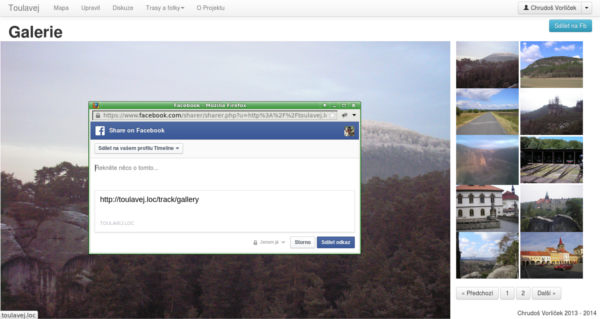
\includegraphics[width=12cm]{obrazky/toulavej/fbShareGallery.png}
				\caption{Příklad sdílení fotografie v~galerii aplikace \uv{Toulavej}}
				\label{fig:fbShare1}
				(zdroj: snímek obrazovky)
			\end{center}
		\end{figure}
	\paragraph{}Před odesláním zprávy na \acl{Fb} je možné nastavit, zda bude zveřejněna na zdi uživatele, ve skupině, na zdi uživatelova kamaráda či v~soukromé zprávě. Dále se dá nastavit, kdo daný příspěvek uvidí, viz obr. \ref{fig:fbShare1}.  Po odeslání se příspěvek zveřejní na \acl{Fb}u, viz obr. \ref{fig:fbShare2}.
		\begin{figure}[!h]
			\begin{center}
				
\includegraphics[width=8cm]{obrazky/toulavej/fbSharefb.png}
				\caption{Výsledný příspěvek na uživatelově zdi na \acl{Fb}u}
				\label{fig:fbShare2}
				(zdroj: snímek obrazovky)
			\end{center}
		\end{figure}				

				\paragraph{} Bylo zjištěno, že pokud se uživatel odhlásí z~aplikace, ale zůstane stále přihlášen na Facebooku, může zveřejňovat věci na zdi. V~momentě, kdy se na počítači střídá víc lidí, může dojít k~situaci, kdy jeden uživatel, který vůbec nemusí mít účet na Facebooku, bude moci publikovat statusy na zdi někoho, kdo byl na počítači před ním a zapomněl se odhlásit z~Facebooku. Protože toto je nežádoucí jev, byla proti němu učiněna opatření v~podobě skrytí tlačítka, které sdílení vyvolává. Tlačítko se zobrazí jen v~případě, že má uživatel u~svého účtu uloženo v~databázi \textit{fbuid}, což je označení pro pole v~tabulce \textit{users}, ve kterém je uložena uživatelská identifikace obdržená z~Facebooku.
		
                                %%% ML: zmenil jsem nazev kapitoly na
                                %%% OSM, jinak to bylo prilis obecne

		\section{Editace dat OSM}

                %%% ML: zde by se hodil odkaz na kapitolu o iD
		%%% ChV: doplněn do textu k první zmínce

				\paragraph{} Pro umožnění editace dat existovala dvě možná řešení. První řešení zahrnuje vytvoření vlastního rozhraní, druhé pak použití existujícího řešení a připojení k~vlastní webové aplikaci. U~druhého řešení byla od začátku zvažována možnost použití HTML5 editoru \textit{iD}, viz kap. \ref{sec:editory}. Protože obě řešení mají své výhody a nevýhody, budou zde vypsány obě.
			\subsection{Tvorba vlastního rozhraní}
				\paragraph{} První řešení, jak už bylo řečeno, zahrnuje vytvoření jednoduchého rozhraní. Prvky by se editovaly a  ukládaly do databáze projektu a v~určitých intervalech by byl prováděn import těchto dat do OpenStreetMap. Výhoda této metody spočívá v~tom, že data by mohla být kontrolována, zda jsou fakticky správně, aby nedocházelo k~znehodnocení dat OpenStreetMap. Také by bylo možno tuto funkci implementovat s~minimálními změnami pro přidávání vlastních cest. Na druhou stranu by toto řešení znamenalo množství programování, protože by bylo potřeba zajistit nástroj pro import do OpenStreetMap, popřípadně data importovat ručně. V~začátcích by to pravdě\-podobně nebyl problém, ovšem po překročení určitého počtu editací by se mohl stát ruční import nemožným nebo alespoň velice náročným na čas.
				\paragraph{} Protože zde nedochází k~odesílání dat na jiný server, byl tento přístup zvolen pro přidávání vlastních cest a fotografií.
			\subsection{Editor iD} 
				\paragraph{} Kvůli výše vyjmenovaným nevýhodám bylo rozhodnuto, že nejprve bude prozkoumána možnost připojení HTML5 editoru \textit{iD}, který byl vytvořen pro editaci dat OpenStreetMap. Po prozkoumání zdrojových kódů editoru bylo zjištěno, že aplikace může být připojena a že autorizace uživatele probíhá pomocí protokolu \textit{oAuth}. Aby aplikace nepoužívala osobní účet na \acl{OSM}, byl vytvořen speciální účet, pod kterým aplikace byla registrována. 

		\begin{figure}[!h]
			\begin{center}
				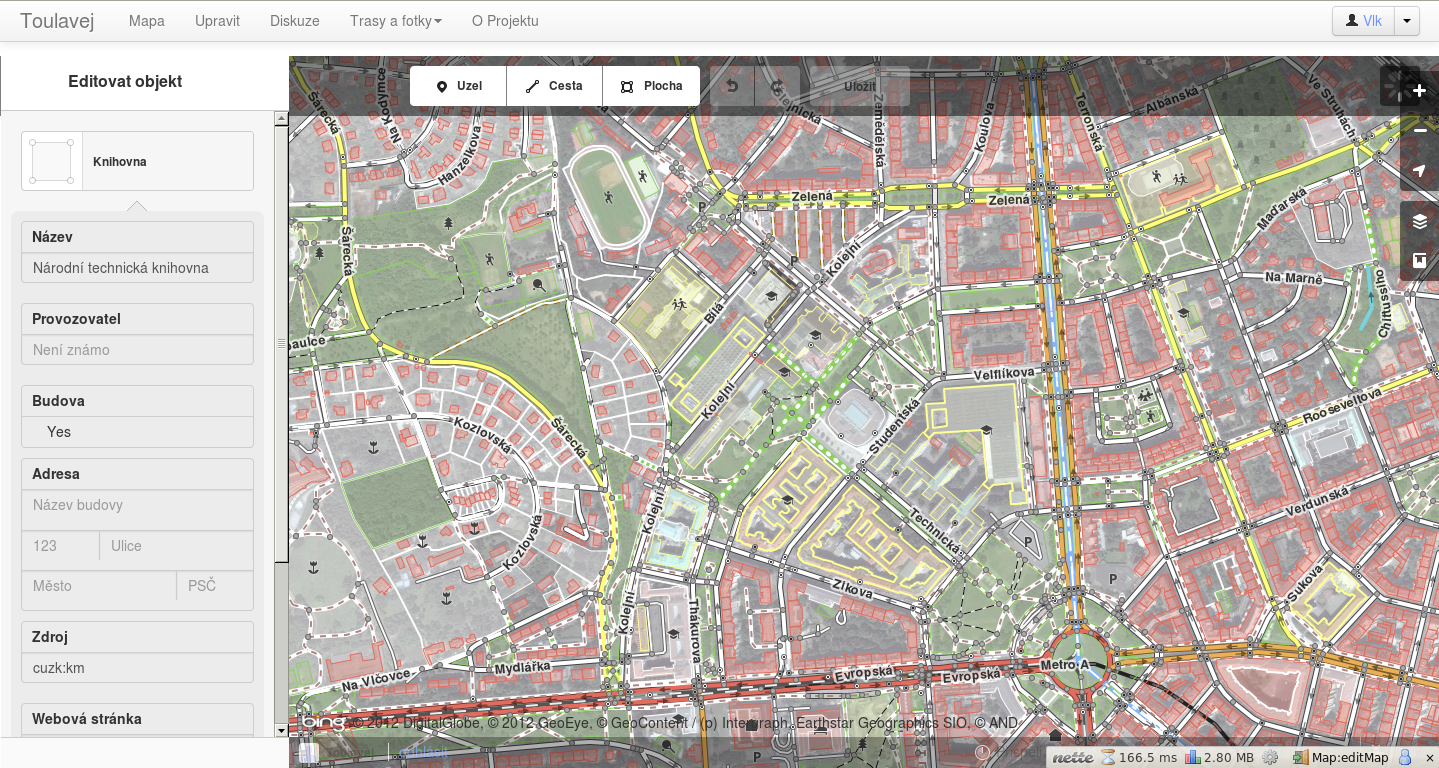
\includegraphics[width=12cm]{obrazky/toulavej/idToulavej.png}
				\caption{Editor iD v~aplikaci \uv{Toulavej}}
				\label{fig:idToulavej}
				(zdroj: snímek obrazovky)
			\end{center}
		\end{figure}	

                 %%% ML: proc zmena velikosti fontu ???
		  %%% ChV: pouze aby mi v textu neuniklo, že je to nekompletní či spíše na přepsání
				\paragraph{} Dle původního plánu měla aplikace umožnit editaci i uživatelům, kteří nemají účet na \acl{OSM}. Tento záměr byl ale opuštěn, protože by mohlo dojít k~zneužití účtu aplikace pro znehodnocení dat \acl{OSM}. Z~toho důvodu mohou data editovat jen uživatelé, kteří mají na \ac{OSM} účet.
				\paragraph{} Při autentizaci přes oAuth docházelo k~chybě při zpětném přesměrování. Tento problém byl vyřešen nastavením zpětné adresy do šablony s~javascriptovým kódem, který vykonal dokončení autentizace a přesměroval uživatele na správnou adresu.

				\paragraph{} Editor iD má i určité nevýhody. Například poskytuje více funkcionalit než je potřeba a komplexnost editoru činí modifikaci zdrojového kódu časově náročnou. Pro vytvářenou aplikaci je nadbytečná možnost editace budov. V~momentě, kdy by nebyla povolena editace plošných prvků (polygonů), probíhalo by načítání dat z~OpenStreetMap rychleji. 



		\section{Trasy a fotografie}
                %%% ML: TODO
			\subsection{Trasy}
			\paragraph{} V~sekci \textit{Dostupné funkce},viz kap. \ref{sec:funkce}, bylo řečeno, že si uživatel může prohlížet trasy a v~případě, že je přihlášený, může je sám přidávat. Tato funkcionalita by měla sloužit jako zdroj inspirace pro ostatní uživatele. Z~toho důvodu je možné psát k~jednotlivým trasám i komentáře ohledně obtížnosti trasy, celkového pocitu z~ní a dalších postřehů. Tyto informace se pak zobrazí v~detailních informacích o~trase, viz obr. \ref{fig:tDetail}. Kromě nich je zde i odkaz na zobrazení trasy na mapě.
		\begin{figure}[!h]
			\begin{center}
				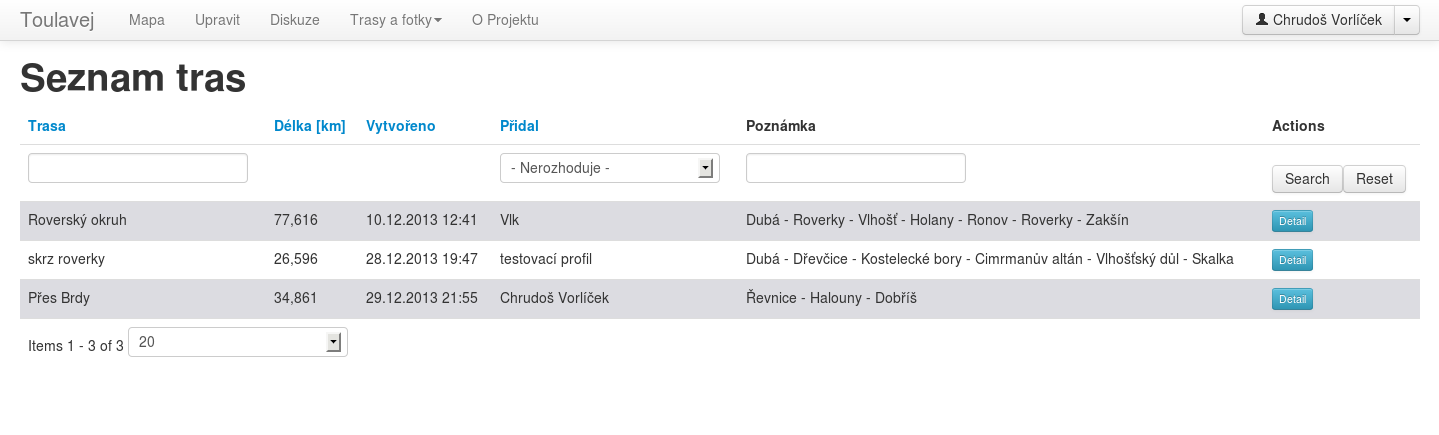
\includegraphics[width=12cm]{obrazky/toulavej/trackDefault.png}
				\caption{Seznam tras v~databázi aplikace \uv{Toulavej}}
				\label{fig:tDefault}
				(zdroj: snímek obrazovky)
			\end{center}
		\end{figure}	
		\paragraph{} Pro vytvoření seznamu s~možností výběru dle zadaných parametrů byl použit plugin Grido, viz obr. \ref{fig:tDefault}. Kromě třídění položek umí tento doplněk i řadit data podle zvoleného parametru. Ze seznamu je u~každé položky odkaz na detail trasy.
		\begin{figure}[!h]
			\begin{center}
				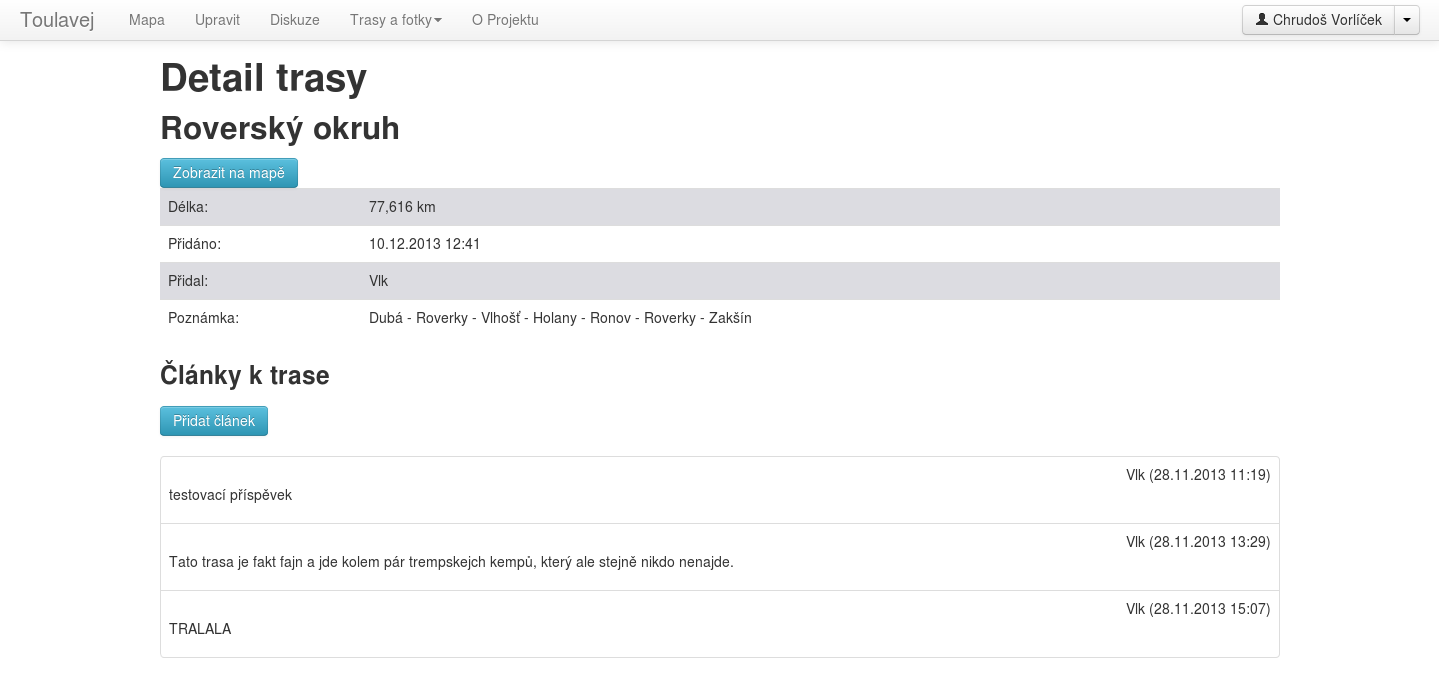
\includegraphics[width=12cm]{obrazky/toulavej/trackDetail.png}
				\caption{Detailní zobrazení informací o~trase spolu s~komentáři}
				\label{fig:tDetail}
				(zdroj: snímek obrazovky)
			\end{center}
		\end{figure}
		\begin{figure}[!h]
			\begin{center}
				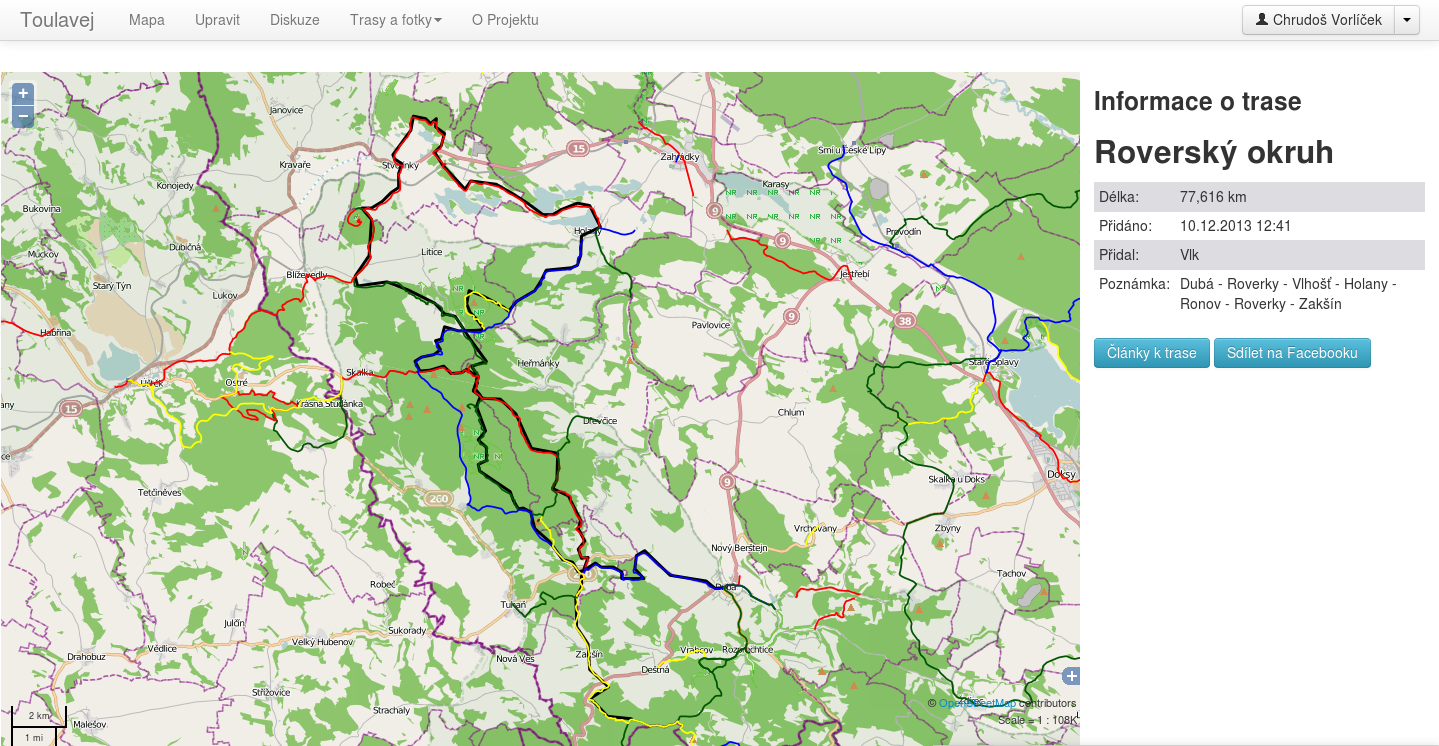
\includegraphics[width=12cm]{obrazky/toulavej/trackTrack.png}
				\caption{Zobrazení trasy v~mapě spolu s~informacemi o~trase}
				\label{fig:tTrack}
				(zdroj: snímek obrazovky)
			\end{center}
		\end{figure}
			\paragraph{} Pro uložení trasy do databáze slouží mapa, která obsahuje funkce umožňující přidávat polylinie, viz obr. \ref{fig:tAdd}. Tato funkce vznikla upravením funkce, kterou využívá ukázkový příklad textit{Modify Feature} na webu OpenLayers.org\cite{ol}. Hlavní rozdíly jsou v~automatickém přepnutí z~vkládání bodů na úpravu trasy po přidání jedné polylinie a předávání geometrie do formuláře (bude zmíněno níže).
			\paragraph{} Po nahrání stránky je uživatel informován, že je editace aktivní a že může začít vkládat body trasy. V~momentě, kdy skončí s~přidáváním bodů, aktivuje se možnost modifikace trasy. Ta umožňuje po kliknutí na trasu mazat a přidávat body a měnit jejich polohu. Před uložením je potřeba trasu pojmenovat. Je možné i vypsat body, kterými trasa prochází. 
			\paragraph{} Na začátku vývoje aplikace se předpokládalo, že na přidání trasy uživatelem bude potřeba použít službu \ac{WFS-T}. Tato strategie je sice možná, ale jednodušším řešením je předání geometrie trasy  formuláři a uložit ji společně s~ostatními daty  do databáze pomocí funkce INSERT.
		\begin{figure}[!h]
			\begin{center}
				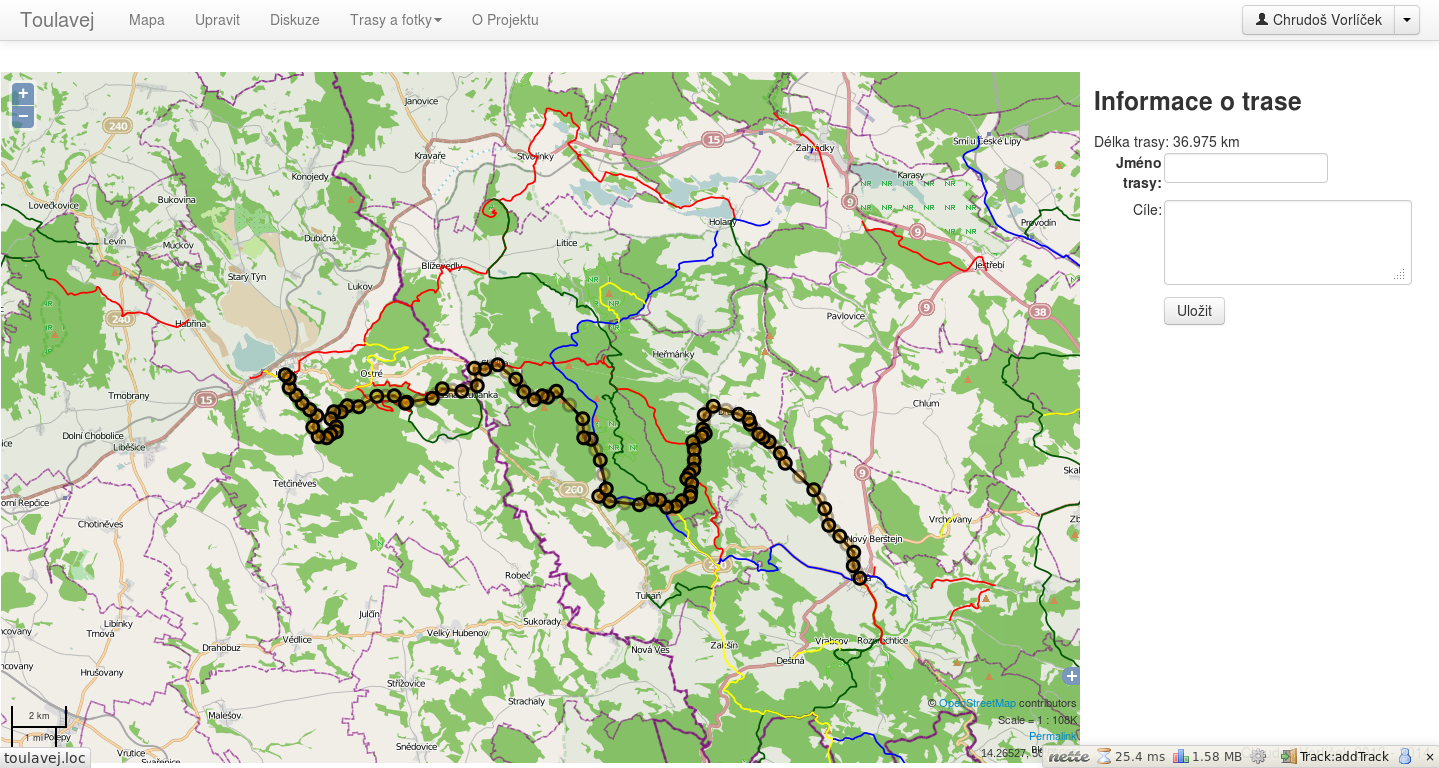
\includegraphics[width=12cm]{obrazky/toulavej/trackAdd.png}
				\caption{Přidávání nové trasy}
				\label{fig:tAdd}
				(zdroj: snímek obrazovky)
			\end{center}
		\end{figure}

		\subsection{Galerie}
			\paragraph{} Aplikace kromě vkládání a zobrazení tras podporuje i vložení a zobrazení fotografií. Pro jejich zobrazení bylo zvažováno použití javascriptové knihovny. Zde ale vznikl problém s~předáváním parametrů pro sdílení obrázků na \acl{Fb}u. Z~toho důvodu byla galerie vytvořena v~PHP tak, aby docházelo k~vypsání \textit{id} v~URL adrese. Další výhodou tohoto řešení byla i lepší kontrola nad vykreslením celé galerie, viz obr. \ref{fig:gallery}.
		\begin{figure}[!h]
			\begin{center}
				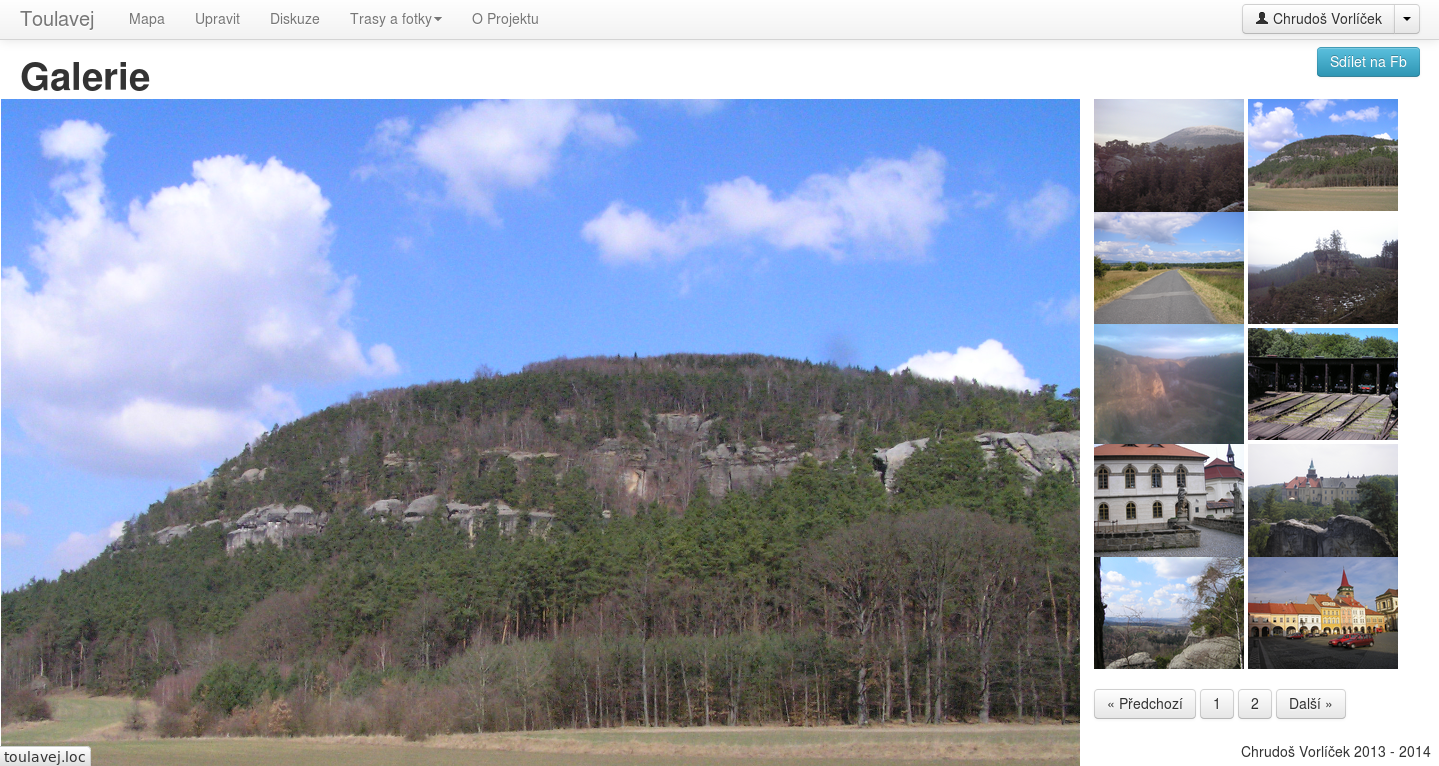
\includegraphics[width=12cm]{obrazky/toulavej/gallery.png}
				\caption{Galerie aplikace \uv{Toulavej}}
				\label{fig:gallery}
				(zdroj: snímek obrazovky)
			\end{center}
		\end{figure}
			\paragraph{} Vrstva fotografií je také připojena spolu s~ostatními vrstvami do hlavní mapové aplikace, viz obr. \ref{fig:vlhost}.

		\begin{figure}[!h]
			\begin{center}
				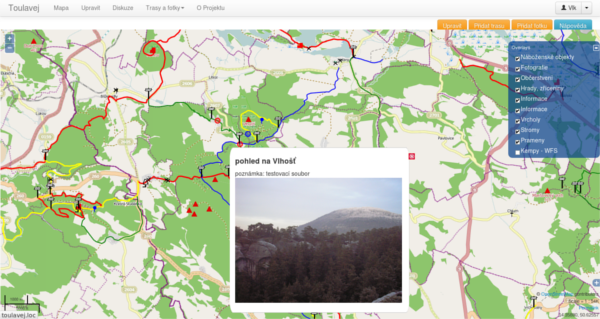
\includegraphics[width=10cm]{obrazky/toulavej/mapa2_vlhost.png}
				\caption{Zobrazení fotografie v~mapě}
				\label{fig:vlhost}
				(zdroj: snímek obrazovky)
			\end{center}
		\end{figure}	

		
			\paragraph{}Postup pro přidání fotografie je podobný jako pro přidání trasy. V~mapě se zvolí bod, odkud daná fotografie pochází, vyplní se jméno a případně popis. Rozdíl mezi přidáním trasy a fotografie je v~tom, že při ukládání fotografie pracujeme se souborem. Pro jeho vybrání slouží tlačítko \textit{Procházet}, které otevře dialogové okno, viz obr. \ref{fig:addImage}. V~momentě potvrzení formuláře se odešle i obrázek. Maximální velikost obrázku je dána nastavením serveru. Na školním serveru je maximální velikost souboru nastavena na 2 MB. Pokud je obrázek větší, k~odeslání formuláře nedojde. Když je formulář validní, dojde k~jeho odeslání na server, kde je fotografie přesunuta do určené složky. Ostatní data, např. jméno souboru a jméno obrázku, jsou uloženy do databáze.
		\begin{figure}[!h]
			\begin{center}
				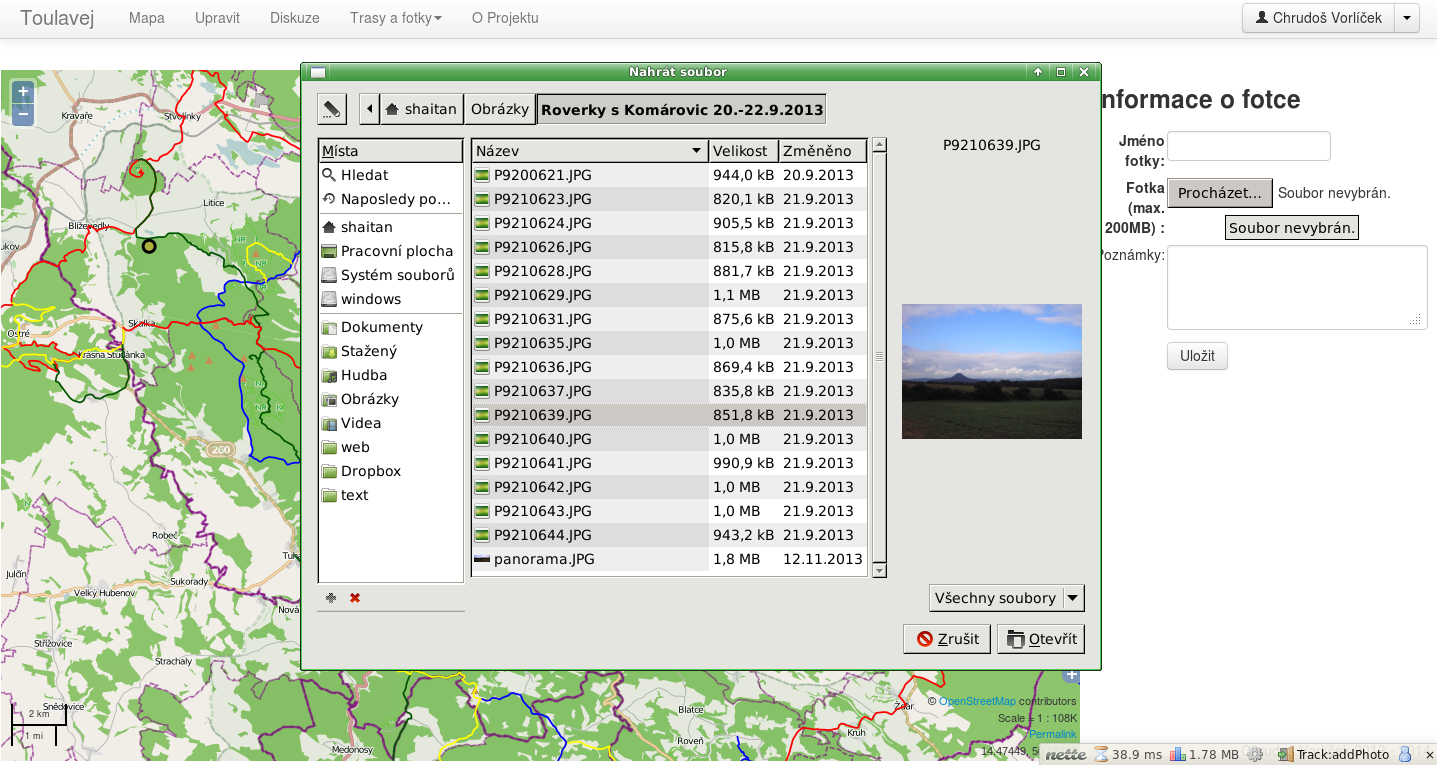
\includegraphics[width=12cm]{obrazky/toulavej/addImage.png}
				\caption{Přidání fotografie s~dialogovým oknem pro výběr}
				\label{fig:addImage}
				(zdroj: snímek obrazovky)
			\end{center}
		\end{figure}


		\section{Testování}
                %%% ML: TODO
		\paragraph{} Tvorba jakékoliv aplikace se neobejde bez chyb. Z~toho důvodu je velice důležité všechny části aplikace testovat a kontrolovat, zda vše v~pořádku funguje. Aplikace \uv{Toulavej} byla testována při vývoji. Kromě zobrazení výpisů jednotlivých proměnných, byly kontrolovány i dotazy na server a jeho odpovědi. V~případě závažných chyb pomohl Nette Debugger, viz kap. \ref{par:ladenka}.
		\paragraph{}I přes to, že aplikace byla několikrát kontrolována a funkce byly testovány, mohou běžní uživatelé  nějaké chyby zaznamenat. Z~toho důvodu byl vytvořen formulář,viz obr. \ref{fig:error}, který odešle administrátorovi mail s~textem. Tento formulář je možné použít i pro zaslání návrhů na vylepšení aplikace. 
		\begin{figure}[!h]
			\begin{center}
				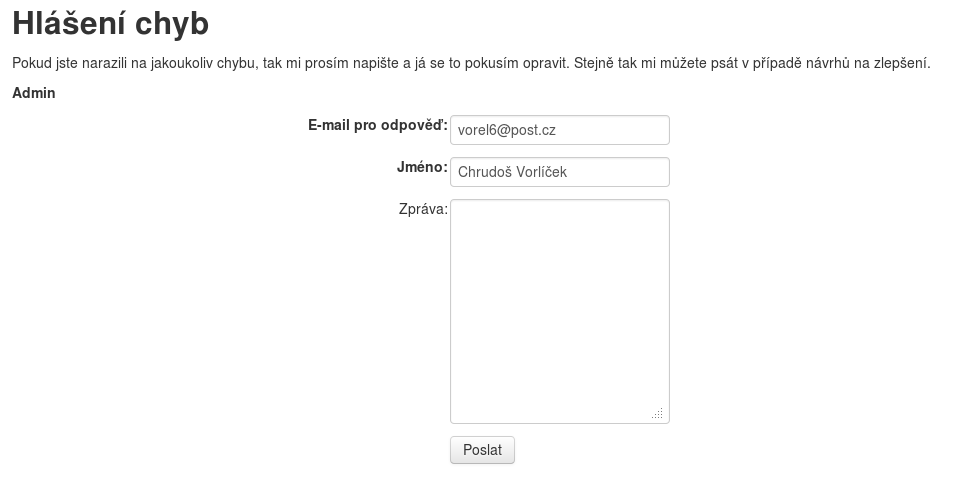
\includegraphics[width=10cm]{obrazky/toulavej/error.png}
				\caption{Formulář pro hlášení chyb}
				\label{fig:error}
				(zdroj: snímek obrazovky)
			\end{center}
		\end{figure}	
		\paragraph{}Tento formulář je stejně jako všechny ostatní chráněn proti spamu. Zejména u~tohoto formuláře je to důležitá funkce, protože k~němu mají přístup přihlášení i nepřihlášení uživatelé. Navíc je napojen na mail, který odesílá zprávy administrátorovi. Pokud by nebyl chráněn a byl napaden robotem rozesílajícím spam, zahltil by administrátorův mail.

		

%%%%%%%%%%%%%%%%%%%%%%%
%%%%% 		ZÁVĚR	  	   %%%%%
%%%%						      %%%%
%%%							  %%%
%%								     %%
%									 %
	\chapter{Zhodnocení}
		\section{Budoucí rozšíření}
			\label{sec:budoucnost}
			\paragraph{}V úvodu jsou definovány vlastnosti, které by aplikace měla splňovat. Všechny hlavní znaky aplikace splňuje, ale současně je zde prostor pro jejich vylepšení. \ac{Fb} poskytuje rozsáhlé \ac{API}, jehož některé funkce by tuto aplikci obohatily. Jedná se zejména o~nahrávání fotografií na uživatelovu zeď či do soukromé zprávy a možnost \uv{dát like} fotkám, trasám či článkům. Jedním z~možných rozšíření je propojení této aplikace se skupinou na \ac{Fb} tak, aby novinky, které se propisují na domovskou stránku aplikace, byly odesílány na zeď této skupiny.
			\paragraph{}\ac{Fb} není jediná sociální síť, tudíž je velice pravděpodobné, že budoucí verze budou podporovat i např. Twitter nebo Google+. Zvláště propojení s~Twitterem je velice pravděpodobné, protože užívá autorizaci přes oAuth stejně jako \acl{OSM}.
			\paragraph{}V současné verzi mohou uživatelé přidat trasy a fotografie, ale už není možné je editovat. Tato funkce se velice hodí, pokud uživatel uloží špatné informace a chce je upravit. Uživatel by také měl mít možnost smazat nebo zneviditelnit fotografie a trasy jím nahrané. Tyto prvky by měly mít při dalším vývoji vysokou prioritu.
			\paragraph{}Další možný vývoj je v~sekci diskuze. Zde by měla přibýt možnost reagovat na jiný příspěvek. Dále by bylo dobré mít možnost zobrazit si příspěvky tak, jak na sebe navazují dle reakcí.
			\paragraph{}V úvodu též byly definovány další funkcionality. V~budoucích verzích programu by se mělo objevit vyhledávání objektů pomocí jejich adresy, vyhledání současné pozice, vyhledávání cest mezi zadanými body a vyhledávání objektů v~určité vzdálenosti od bodu či od cesty. 
			\paragraph{}Rozšířením předchozího vyhledávání je zobrazení fotografií, které jsou podél plánované cesty. Kromě vyhledání cesty je plánováno, že aplikace též spočte výškový profil nalezené cesty. K~tomu bude třeba aplikaci propojit s~modelem terénu.
			\paragraph{}V neposlední řadě je možné upravit zdrojové kódy pro přidávání tras a fotografií tak, aby využívaly co nejvíce společných funkcí.
			\paragraph{}Kromě výše uvedených možností je zde dalších několik věcí, které by aplikaci mohli obohatit. Jedná se mimo jiné o~přidání dalších vrstev zájmových bodů a upravit mapový klíč aplikace v~souladu s~klíčem projektu \acl{OTM}. Také stojí za prozkoumání jak umožnit uživatelům, kteří nemají účet na \ac{OSM}, aby mohli editovat data \ac{OSM}, ale aby byla zachována bezpečnost a nehrozilo znehodnocení mapy \acl{OSM}.
                %%% ML: TODO

		\section{Známé problémy}
		 %%% ML: TODO
			\paragraph{} Ačkoliv se během vývoje povedlo odstranit většinu chyb, aplikace stále nějaké obsahuje. Následující řádky představí ty, které jsou známé a na jejichž odstranění se pracuje.
			\paragraph{} Největším problémem, který ovlivňuje chod celé aplikace, je v~současné době nestabilita Geoserveru na školním serveru geo102. Během vývoje se několikrát stalo, že Geoserver přestal poskytovat služby a nebylo možné přistoupit k~uživatelskému rozhraní. V~případě výpadku Geoserveru dojde k~přerušení všech poskytovaných služeb a místo mapy se na stránce zobrazí růžová plocha. Jedinou mapu, kterou výpadek školního Geoserveru neovlivní, je mapa v~editoru iD, která je připojena z~jiného zdroje.
			\paragraph{} Dalším problémem, se kterým se lze občas setkat, je špatný symbol v~bodové vrstvě. Toto je dáno špatným nastavením VIEW, které vypisuje všechny atributy. U~některých prvků může tak dojít k~tomu, že dva atributy mají hodnotu, které odpovídá nějaké pravidlo, podle kterého se přiřazují symboly. V~tomto případě je objektu přiřazen symbol pravidla, které je jako poslední. Tato chyba bude brzy odstraněna.
			\paragraph{} Spojení stylů editoru iD a aplikace způsobilo kolizi některých pravidel vykreslení prvků. U~většiny prvků se povedlo tyto chyby odstranit, ale stále se objevují nějaké chyby. Za chybu se dá též považovat zobrazení mapy v~iD editoru. Ta je zde velice světlá, takže je na ní občas problematické rozeznat objekty.

		\section{MTB mapa Evropy}

                %%% ML: Mozna by bylo zahodno psat Toulej v uvozovkach
			\paragraph{} V~kapitole \textit{Existující řešení}, viz kap. \ref{sec:Ex_reseni}, je popisována aplikace MTB mapa Evropy, která se věnuje cykloturistice a turistice. Ačkoliv aplikace zobrazují stejná data a jsou určeny pro dosti podobnou skupinu lidí, hlavní téma této práce leží v~jiné oblasti než je tvorba samotné mapy. Projekt \uv{Toulavej} je zaměřen hlavně na propojení se sociální sítí a s~editorem iD. Stránky  nabízí možnost registrace, která poskytuje další výhody, jako je editace dat, přidávání vlastních cest a fotografií. Tyto funkce odlišují obě aplikace a~nedělají z~projektu \uv{Toulavej} pouze další turistickou mapu. Aplikace MTB mapa Evropy byla objevena před odevzdáním této práce, a proto uvedené funkce nemohly být tvořeny jako doplňky pro stávající mapy.

		\section{Výsledná aplikace}
			\paragraph{} Ačkoliv práce na aplikaci budou pokračovat a bude dále vyvíjena, už nyní splňuje vlastnosti, které byly definovány v~\textit{Úvodu}. 
			\paragraph {}Účet na sociální síti se dá použít k~přihlášení, takže si uživatel nemusí pamatovat další heslo a uživatelské jméno. Díky tomuto propojení lze i sdílet s~přáteli zajímavá místa, trasy a fotografie. Dalším bodem bylo umožnění editace dat \ac{OSM}. Tento bod byl asi nejproblematičtější, protože zkoumání a pochopení zdrojových kódů editoru iD zabralo mnoho času. Díky tomu ale bylo možno propojení s~\acl{OSM} realizovat. Vkládání tras a fotografií bylo také realizováno.
			\paragraph{} Funkce a vzhled aplikace byly vyvíjeny s~ohledem na budoucí rozvoj aplikace. V~ideálním příbadě by to znamenalo, že se ve stávajících zdrojových kódech nebude nic měnit, ale využije se z~nich maximum použitelných funkcí.


%% Seznam zkratek
\newpage 
\chapter*{Seznam zkratek}

%%% ML: seznam zkratek se da generovat automatizovane, viz poznamky na
%%% zacatku textu, vzhledem k casovemu tlaku to nechte takto

\addcontentsline{toc}{chapter}{Seznam zkratek}
	\begin{acronym}[WYSIWYG]
		\acro{API}{Application Programming Interface}
		\acro{CGI}{Common Gateway Interface}
		\acro{CSS}{Cascading Style Sheets}
		\acro{cuzk}[ČÚZK]{Český úřad zeměměřický a katastrální}
		\acro{EPSG}{ European Petroleum Survey Group}
		\acro{Fb}{Facebook}
		\acro{GNSS}{Global Navigation Satellite System}
		\acro{GPL}{General Public Licence}
		\acro{GPX}{GPS eXchange format}
		\acro{HTML}{HyperText Markup Language}
		\acro{HTTP}{HyperText Transfer Protocol}
		\acro{JOSM}{Java OpenStreetMap Editor}
		\acro{kct}[KČT]{Klub českých turistů}
		\acro{KML}{Keyhole Markup Language}
		\acro{PHP}{PHP: Hypertext Prepocessor}
		\acro{SLD}{Styled Layer Descriptor}
		\acro{SVG}{Scalable Vector Graphics}
		\acro{OSM}{OpenStreetMap}
		\acro{ODbL}{Open Database License}
		\acro{OTM}{OpenTrackMap}
		\acro{uhul}[ÚHUL]{Ústav pro hospodářskou úpravu lesů}
		\acro{UI}{User Interface}
		\acro{XML}{eXtended Markup Language}
		\acro{WFS}{Web Feature Service}
		\acro{WFS-T}{Web Feature Service -- Transactional}
		\acro{WGS 84}{World Geodetic System 1984}
		\acro{WMS}{Web Map Service}
		\acro{WTFPL}[WTFPL]{Do What The Fuck You Want To Public License}
		\acro{WYSIWYG}{What You See Is What You Get}
	\end{acronym}

%%Užitá literatura

%%% ML: Literatura by mela byt rozdelene na dve sekce - primarni
%%% (tistena a clanky) a sekundarni (online) - casu je malo a zbyva
%%% Vam hodne nedodelku, nechte to v nejhorsim pripade takto, jenom
%%% dejte do textu vice odkazu na literaturu, to tam velmi chybi, viz
%%% poznamky v textu

%%% ML: Pokud by zbyl cas tak pridejte do prace dodatek s doplnujicimi
%%% informacemi, napr. podstatne casti konfigurace ci popis aplikace
%%% se vice screenshoty, bohuzel ale neni prilis casu a stale vam
%%% chybi zasadni casti prace...

\newpage
\addcontentsline{toc}{chapter}{Reference}
\begin{thebibliography}{99}
	\bibitem{OTM} BARTOŇ, Radek. Custom OpenStreetMap Rendering: OpenTrackMap Experience. In: [online]. 2009. vyd. [cit. 2013-11-12]. Dostupné z:  \url{http://geoinformatics.fsv.cvut.cz/gwiki/Custom_OpenStreetMap_Rendering_-_OpenTrackMap_Experience}
	\bibitem{crockford}CROCKFORD, Douglas. JavaScript: The World's Most Misunderstood Programming Language. Douglas Crockford's Wrrrld Wide Web [online]. 2001 [cit. 2014-01-03]. Dostupné z: \url{http://javascript.crockford.com/javascript.html}
	\bibitem{dp_dolezal}DOLEŽAL, Jan. Datové formáty pro prezentaci map na webu [online]. Praha, 2005 [cit. 2014-01-03]. Dostupné z: \url{http://geo3.fsv.cvut.cz/~soukup/dip/dolezel/}. Diplomová práce. ČVÚt v~Praze. Vedoucí práce Ing. Petr Soukup, Ph.D.
	\bibitem{rfc2616}FIELDING, Roy et al. RFC 2616: Hypertext Transfer Protocol HTTP/1.1. In: IETF [online]. Fremont(Kalifornie): IETF, June 1999 [cit. 2014-01-03]. Dostupné z: \url{http://tools.ietf.org/html/rfc2616}
        \bibitem{jakPsatWeb}JANOVSKÝ, Dušan. JavaScript: úvod. Jak psát web [online]. [cit. 2014-01-03]. Dostupné z: \url{http://www.jakpsatweb.cz/javascript/javascript-uvod.html}
	\bibitem{nette20login}MAREK, Jakub: Přihlašování v~Nette Frameworku [online].  [cit. 2013-10-29]. Dostupné z: \url{http://github.com/janmarek/nette20login}
	\bibitem{neis}NEIS, Pascal. The OpenStreetMap Contributors Map aka Who’s around me?. In: [online]. [cit. 2013-12-14]. Dostupné z: \url{http://neis-one.org/2013/01/oooc/}
	\bibitem{FbTools} ŠULC, Milan: FbTools [online].  [cit. 2013-10-29]. Dostupné z: \url{http://addons.nette.org/cs/fb-tools}.
	\bibitem{tesar_bp}TESAŘ, Martin. Vykreslovací systém MTB map pro OpenStreetMap. Brno, 2010. Dostupné z: \url{http://is.muni.cz/th/256369/fi_b/bpfinal.pdf}. Bakalářská práce. Masarykova univerzita. Vedoucí práce RNDr. Petr Holub, Ph.D.
	\bibitem{bootstrap}Bootstrap [online].  [cit. 2013-10-29]. Dostupné z: \url{http://getbootstrap.com}.
	\bibitem{FbApiPrava} Facebook developers - Login Reference [online]. [cit. 2013-10-21]. Dostupné z: \url{https://developers.facebook.com/docs/reference/login/#permissions}.
	\bibitem{geofabrik}Geofabrik [online]. [cit. 2013-12-14] Dostupné z: \url{http://download.geofabrik.de/}.
	\bibitem{atlas}GeoPublishing: AtlasStyler SLD editor [online]. [cit. 2013-11-13]. Dostupné z: \url{http://en.geopublishing.org/AtlasStyler}
	\bibitem{geoserver}Geoserver [online]. [cit. 2013-11-13]. Dostupné z: \url{http://geoserver.org/display/GEOS/Welcome}
	\bibitem{Leaflet}	Leaflet - A~JavaScript Library for Mobile-Friendly Maps [online]. [cit. 2013-10-29]. Dostupné z: \url{http://leafletjs.com/}
	\bibitem{netcraft_survey}June 2013 web server survey. Netcraft [online]. Bath: Netcraft Ltd, 2014 [cit. 2014-01-03]. Dostupné z: \url{http://news.netcraft.com/archives/2013/06/06/june-2013-web-server-survey-3.html}
	\bibitem{googleMap}Mapy Google. Google [online]. Mountain View(CA): Google Inc., 2014 [cit. 2014-01-02]. Dostupné z: \url{https://www.google.com/maps/preview#!data=!1m4!1m3!1d81081!2d14.4545573!3d50.5752824}
	\bibitem{vyletnik}Mapy: Mapy - Turistická mapa ČR, mapy turistických tras a cyklotras. Vyletník [online]. Praha: Paseo s.r.o., 2014 [cit. 2014-01-02]. Dostupné z: \url{http://mapy.vyletnik.cz/}
	\bibitem{vyletnikMapa}Mapy: Mapy - Turistická mapa ČR, mapy turistických tras a cyklotras. Vyletník [online]. Praha: Paseo s.r.o., 2014 [cit. 2014-01-02]. Dostupné z: \url{http://mapy.vyletnik.cz/#x=50.59021193935189@y=14.451141357421875@z=11}
	\bibitem{seznamMapa}Mapy.cz. Mapy.cz [online]. Praha: Seznam.cz a.s., 1996-2014 [cit. 2014-01-02]. Dostupné z: \url{http://mapy.cz/#!x=14.532125&y=50.565813&z=11&l=16&c=f-c&d=foto_155656_1&t=s}	
	\bibitem{nette_web}NETTE FOUNDATION. Nette Framework [online]. 2008. vyd. [cit. 2013-12-16]. Dostupné z: \url{http://nette.org} 
	\bibitem{ODbL}Open Data Commons Open Database License (ODbL). Open Data Commons [online]. Cambridge: Open Knowledge Foundation [cit. 2014-01-02]. Dostupné z: \url{http://opendatacommons.org/licenses/odbl/}		
	\bibitem{license}OpenStreetMap Wiki contributors: Cs:ODbL/We Are Changing The License. In: OpenStreetMap Wiki [online]. [cit. 2014-01-02]. Dostupné z: \url{http://wiki.openstreetmap.org/wiki/Cs:ODbL/We_Are_Changing_The_License}
	\bibitem{wiki_comparison}OpenStreetMap Wiki contributors: Comparison of editors In: OpenStreetMap Wiki [online]. [cit. 2013-12-16]. Dostupné z:	\url{https://wiki.openstreetmap.org/wiki/Comparison_of_editors}
	\bibitem{wiki_hot}OpenStreetMap Wiki contributors: Humanitarian OSM Team  In: OpenStreetMap Wiki [online]. [cit. 2013-12-16]. Dostupné z: \url{http://wiki.openstreetmap.org/wiki/Humanitarian_OSM_Team}
	\bibitem{wiki_iD}OpenStreetMap Wiki contributors: iD. In: OpenStreetMap Wiki [online]. [cit. 2013-12-15]. Dostupné z:  \url{http://wiki.openstreetmap.org/wiki/ID}
	\bibitem{wiki_josm}OpenStreetMap Wiki contributors:JOSM. In: OpenStreetMap Wiki [online]. [cit. 2013-12-16]. Dostupné z:  \url{http://wiki.openstreetmap.org/wiki/JOSM}
	\bibitem{wiki_merkaator}OpenStreetMap Wiki contributors: Merkaator. In: OpenStreetMap Wiki [online]. [cit. 2013-12-16]. Dostupné z:  \url{http://wiki.openstreetmap.org/wiki/Merkaator}
	\bibitem{mtb_map-wiki}OpenStreetMap Wiki contributors:  MTB map Europe. In OpenStreetMap Wiki [online]. [cit. 2013-12-11]. Dostupné z:\url{http://wiki.openstreetmap.org/wiki/MTB_map_Europe}.
	\bibitem{osm_wiki_node}OpenStreetMap Wiki contributors: Node In: OpenStreetMap Wiki [online]. [cit. 2014-01-02]. Dostupné z: \url{http://wiki.openstreetmap.org/wiki/Node}
	\bibitem{nominatim}OpenStreetMap Wiki contributors: Nominatim. In OpenStreetMap Wiki [online]. [cit. 2013-12-14]. Dostupné z: \url{http://wiki.openstreetmap.org/wiki/Nominatim}	
	\bibitem{osm}OpenStreetMap contributors: OpenStreetMap In:  [online]. [cit. 2014-01-02]. Dostupné z:	\url{https://wiki.openstreetmap.org}
	\bibitem{osm_edit}OpenStreetMap contributors: OpenStreetMap In:  [online]. [cit. 2014-01-02]. Dostupné z:	\url{http://www.openstreetmap.org/edit}
	\bibitem{planet.osm}OpenStreetMap Wiki contributors: Planet.osm. In OpenStreetMap Wiki [online]. [cit. 2013-12-15]. Dostupné z: \url{http://wiki.openstreetmap.org/wiki/Planet.osm}.
	\bibitem{wiki_p2}OpenStreetMap Wiki contributors: Potlatch 2. In: OpenStreetMap Wiki [online]. [cit. 2013-12-16]. Dostupné z:  \url{http://wiki.openstreetmap.org/wiki/Potlatch2}
	\bibitem{osm_wiki_ramoth}OpenStreetMap Wiki contributors: Servers/Ramoth In: OpenStreetMap Wiki [online]. [cit. 2014-01-02]. Dostupné z:\url{http://wiki.openstreetmap.org/wiki/Servers/ramoth}
	\bibitem{osm_wiki_relation}OpenStreetMap Wiki contributors: Relation In: OpenStreetMap Wiki [online]. [cit. 2014-01-02]. Dostupné z: \url{http://wiki.openstreetmap.org/wiki/Relation}
	\bibitem{osm_wiki_smaug}OpenStreetMap Wiki contributors: Servers/Smaug In: OpenStreetMap Wiki [online]. [cit. 2014-01-02]. Dostupné z:\url{http://wiki.openstreetmap.org/wiki/Servers/smaug}
	\bibitem{osm_wiki_planet.gpx}OpenStreetMap Wiki contributors: Planet.gpx In: OpenStreetMap Wiki [online]. [cit. 2014-01-02]. Dostupné z: \url{http://wiki.openstreetmap.org/wiki/Planet.gpx}
	\bibitem{osm_wiki_stats}OpenStreetMap Wiki contributors: Stats In: OpenStreetMap Wiki [online]. [cit. 2014-01-02]. Dostupné z: \url{http://wiki.openstreetmap.org/wiki/Stats}
	\bibitem{wiki_tajfun}OpenStreetMap Wiki contributors: Typhoon Haiyan In: OpenStreetMap Wiki [online]. [cit. 2013-12-16]. Dostupné z: \url{wiki.openstreetmap.org/wiki/Typhoon_Haiyan_(2013)}
	\bibitem{osm_wiki_way}OpenStreetMap Wiki contributors: Way In: OpenStreetMap Wiki [online]. [cit. 2014-01-02]. Dostupné z: \url{http://wiki.openstreetmap.org/wiki/Way}
	\bibitem{freemap}OpenStreetMap Wiki contributors: WIKIProject Czech Republic/freemap. In: OpenStreetMap Wiki [online]. [cit. 2013-12-15]. Dostupné z:  \url{http://wiki.openstreetmap.org/wiki/WikiProject_Czech_Republic/freemap}
	\bibitem{otm_klic} OpenStreetMap Wiki contributors: WIKIProject Czech Republic/OTM značkový klíč. In: OpenStreetMap Wiki [online]. [cit. 2013-12-12]. Dostupné z: 	\url{http://wiki.openstreetmap.org/wiki/WikiProject_Czech_Republic/OTM_zna%C4%8Dkov%C3%BD_kl%C3%AD%C4%8D}
	\bibitem{ol}OPEN SOURCE GEOSPATIAL FOUNDATION. OpenLayers: Free Maps for the Web [online]. [cit. 2013-12-17]. Dostupné z: \url{http://openlayers.org} 
	\bibitem{php_net}PHP: Hypertext preprocessor [online]. The PHP Group, 2001-2014 [cit. 2014-01-03]. Dostupné z: \url{http://php.net/}
	\bibitem{PostgreSQL} PostgreSQL: The world's most advanced open source database [online]. [cit. 2013-11-08]. Dostupné z: \url{http://www.postgresql.org/}.
	\bibitem{qgis}QGIS [online]. [cit. 2013-11-13]. Dostupné z: \url{http://www.qgis.org/en/site/}
	\bibitem{sphericalMercator}Spherical Mercator. OpenLayers: Free Maps for the Web [online]. Beaverton(Oregon): Open Source Geospatial Foundation, 2008 [cit. 2014-01-02]. Dostupné z: \url{http://docs.openlayers.org/library/spherical_mercator.html}
	\bibitem{apache}The Apache Software Foundation: Apache - HTTP Server project [online]. [cit. 2013-11-12]. Dostupné z: \url{http://httpd.apache.org/}
	\bibitem{creative_commons}Uveďte autora-Zachovejte licenci 2.0 Generic. CREATIVE COMMONS. [online]. [cit. 2013-12-15]. Dostupné z: \url{http://creativecommons.org/licenses/by-sa/2.0/deed.cs}
	\bibitem{Waymarked} Waymarked Trails [online].  [cit. 2013-11-12]. Dostupné z: \url{http://www.waymarkedtrails.org/cs/}
	\bibitem{wiki-Apache}Wikipedia:Apache HTTP Server [online]. [cit. 2013-11-12]. Dostupné z: \url{http://en.wikipedia.org/wiki/Apache_HTTP_Server}	
       \bibitem{wiki_framework}Software Framework. In: Wikipedia: the free encyclopedia [online]. San Francisco (CA): Wikimedia Foundation, 2001- [cit. 2014-01-03]. Dostupné z: \url{http://en.wikipedia.org/wiki/Software_framework}	
	\bibitem{google_wiki}Google Maps. In: Wikipedia: the free encyclopedia [online]. San Francisco (CA): Wikimedia Foundation, 2001- [cit. 2013-12-12]. Dostupné z: \url{http://en.wikipedia.org/wiki/Google_Maps}
       	\bibitem{wiki_js}JavaScript. In: Wikipedia: the free encyclopedia [online]. San Francisco (CA): Wikimedia Foundation, 2001- [cit. 2014-01-03]. Dostupné z: \url{http://en.wikipedia.org/wiki/JavaScript}
       \bibitem{wiki_street_view} Google Street View. In: Wikipedia: the free encyclopedia [online]. San Francisco (CA): Wikimedia Foundation, 2001- [cit. 2014-01-02]. Dostupné z: \url{http://en.wikipedia.org/wiki/Street_view}
	\bibitem{wiki_php}PHP. In: Wikipedia: the free encyclopedia [online]. San Francisco (CA): Wikimedia Foundation, 2001- [cit. 2014-01-03]. Dostupné z: \url{http://en.wikipedia.org/wiki/PHP}
	\bibitem{wiki_postgresql}PostgreSQL. In: Wikipedia: the free encyclopedia [online]. San Francisco (CA): Wikimedia Foundation, 2001- [cit. 2013-12-16]. Dostupné z: \url{http://en.wikipedia.org/wiki/PostgreSQL}
	\bibitem{wiki_ol}OpenLayers. In: Wikipedia: the free encyclopedia [online]. San Francisco (CA): Wikimedia Foundation, 2001- [cit. 2013-12-16]. Dostupné z: \url{http://en.wikipedia.org/wiki/OpenLayers}
	\bibitem{osm_wikipedia_cs}OpenStreetMap. In: Wikipedia: the free encyclopedia [online]. San Francisco (CA): Wikimedia Foundation, 2001- [cit. 2013-12-15]. Dostupné z: \url{http://cs.wikipedia.org/wiki/OpenStreetMap}
	\bibitem{osm_wikipedia_en}OpenStreetMap. In: Wikipedia: the free encyclopedia [online]. San Francisco (CA): Wikimedia Foundation, 2001- [cit. 2013-12-15]. Dostupné z: \url{http://en.wikipedia.org/wiki/OpenStreetMap}
	\bibitem{wiki_webServer}Web Server. In: Wikipedia: the free encyclopedia [online]. San Francisco (CA): Wikimedia Foundation, 2001- [cit. 2013-12-15]. Dostupné z:\url{http://en.wikipedia.org/wiki/Web_server}
	\bibitem{wiki_wtfpl} WTFPL. In: Wikipedia: the free encyclopedia [online]. San Francisco (CA): Wikimedia Foundation, 2001- [cit. 2013-12-15]. Dostupné z: \url{http://en.wikipedia.org/wiki/WTFPL}
	\bibitem{w3school}W3 Schools: Online Web Tutorials [online]. Refsnes Data., 1999-2014 [cit. 2014-01-03]. Dostupné z: \url{http://www.w3schools.com}
\end{thebibliography}
\end{document}
